\documentclass[12pt]{article} %corpo documento a 12, corpo piè di pagina a 10
\renewcommand{\baselinestretch}{1.5} %interlinea a 1.5
\usepackage{graphicx} % Required for inserting images
\usepackage[hidelinks]{hyperref}
\usepackage{setspace}
\usepackage{media9}
\usepackage{float}

\begin{document}

\begin{titlepage}
    \begin{spacing}{0.8}
    \begin{center}
        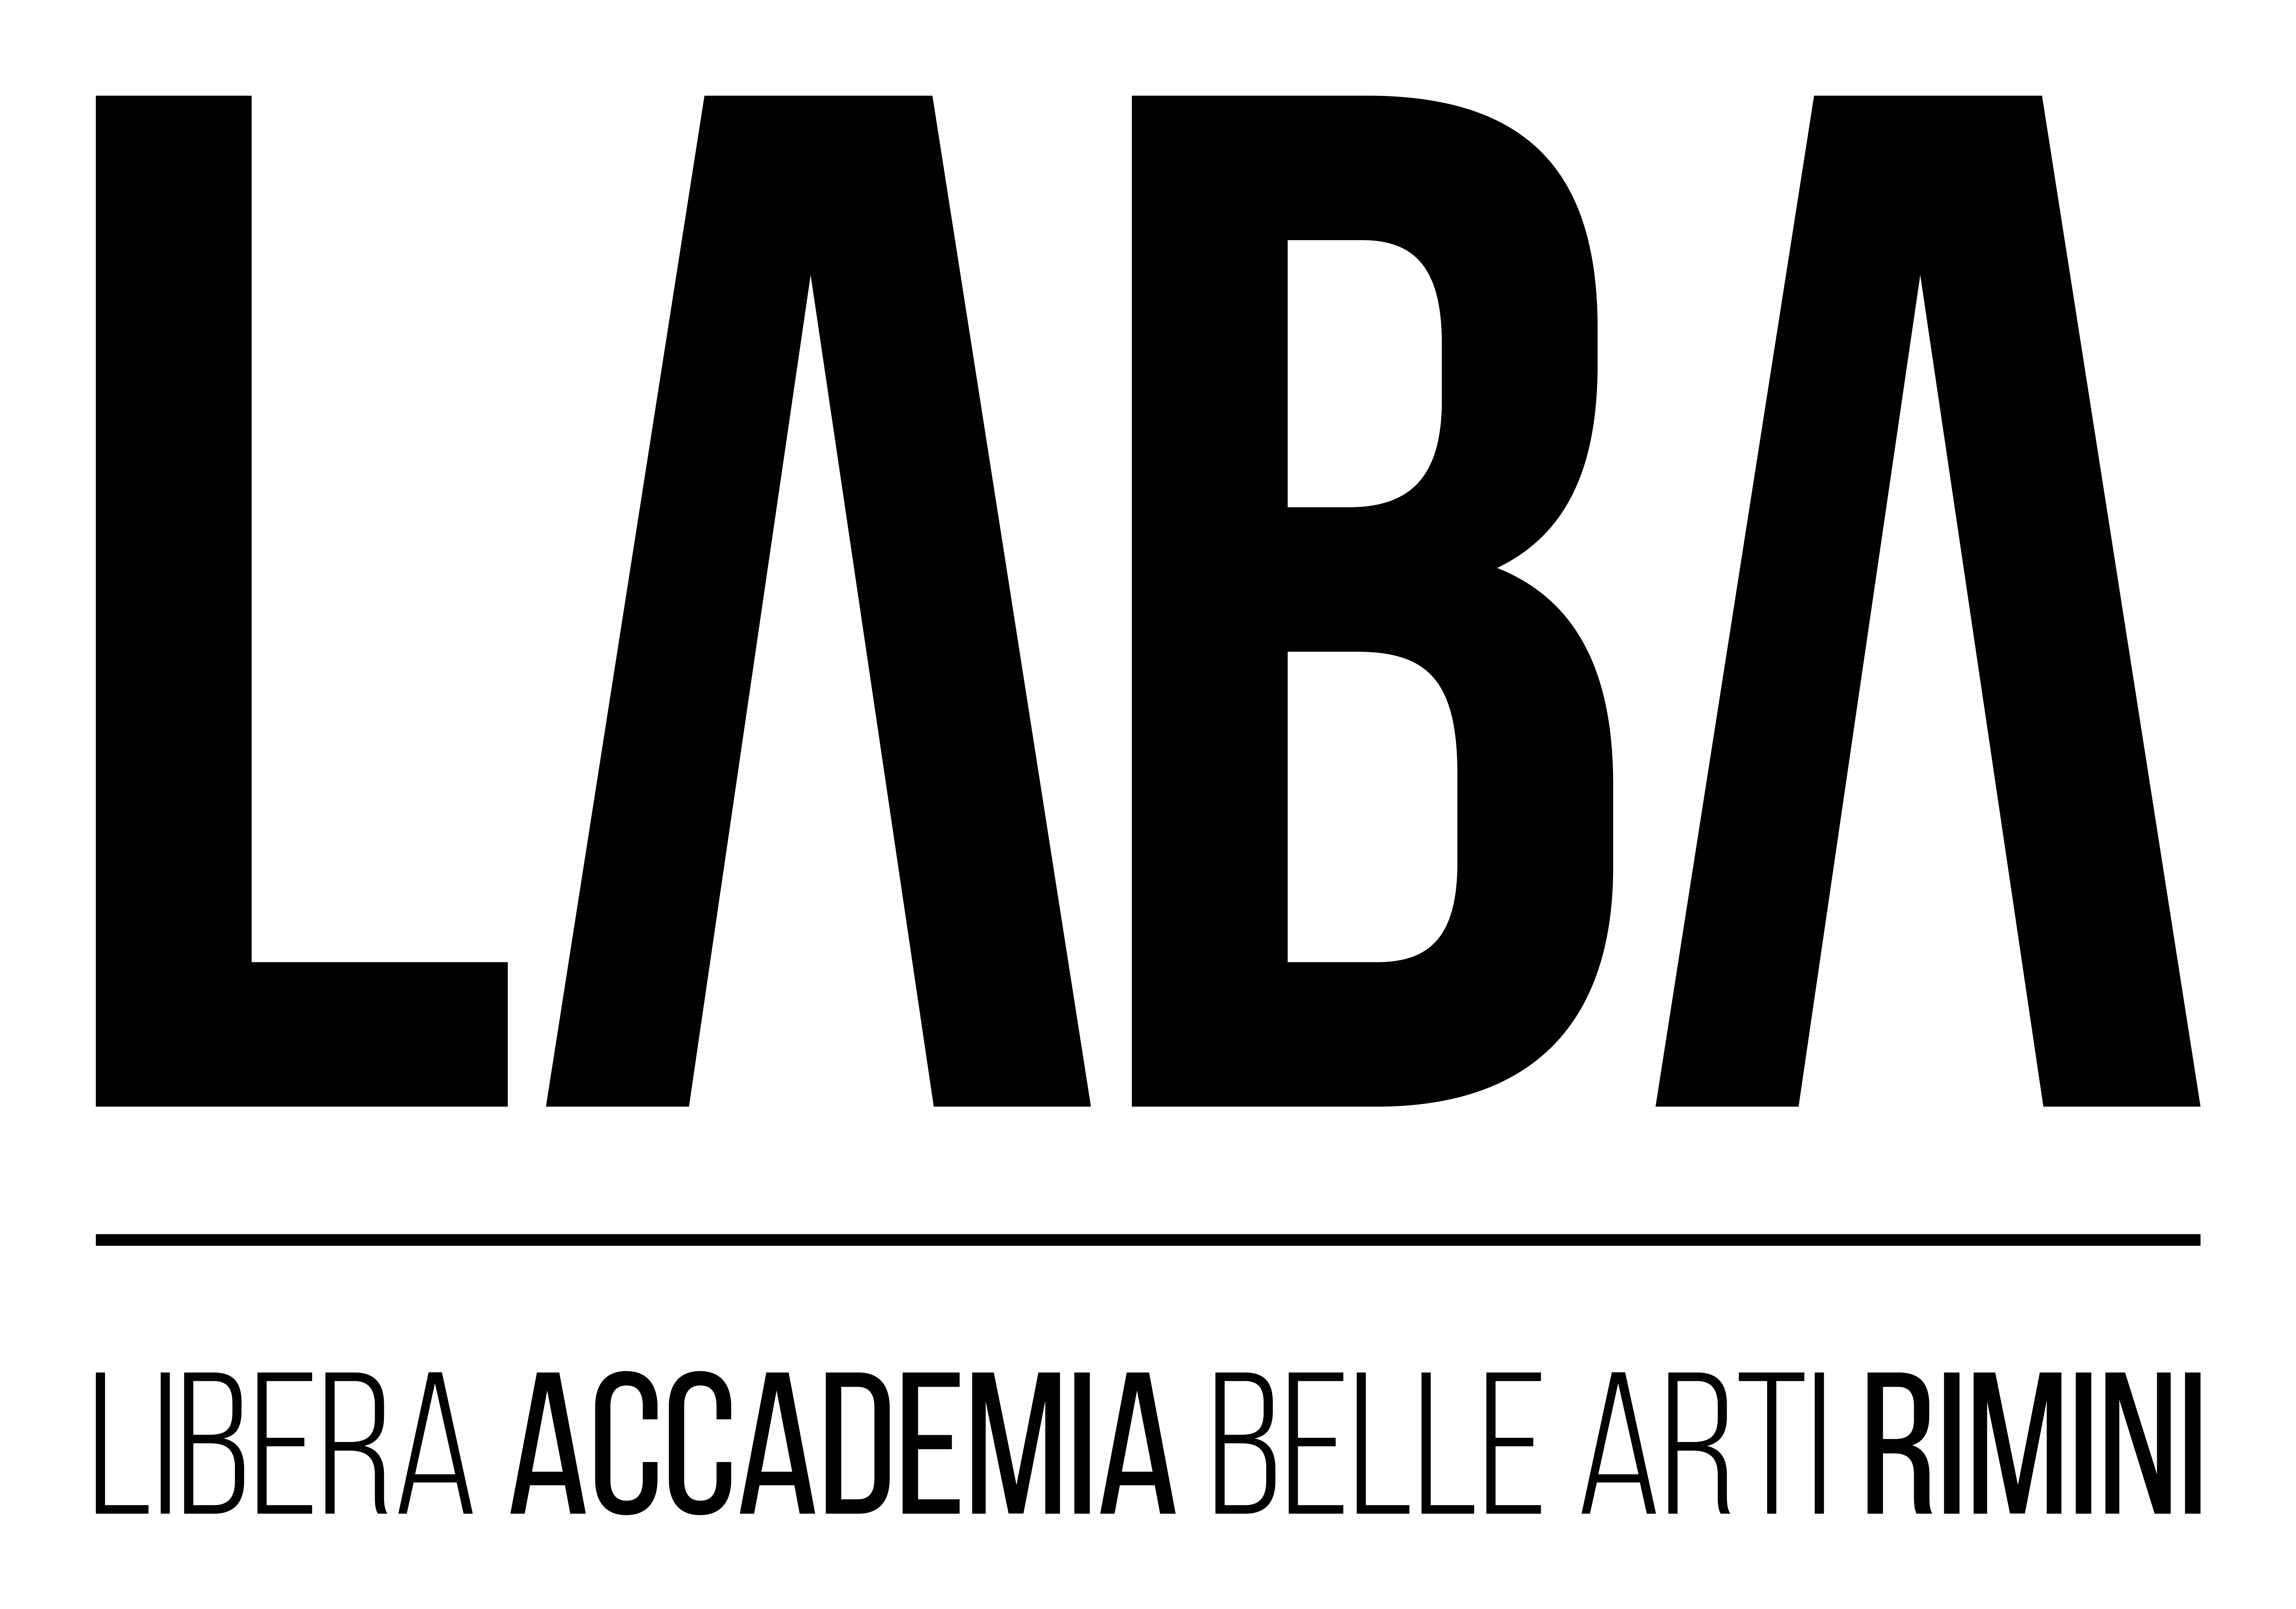
\includegraphics[height=3cm]{labalogo.png}
        \vspace*{1cm}

        \centering{LABA\\\vspace{0.1cm}
        LIBERA ACCADEMIA DI BELLE ARTI\\\vspace{0.1cm}
        SEDE RIMINI \\\vspace{0.5cm}
        DIPLOMA ACCADEMICO DI I LIVELLO\\\vspace{0.1cm}
        IN\\\vspace{0.1cm}
        \textbf{CINEMA, FOTOGRAFIA E AUDIOVISIVO}}

        \vspace*{2cm}
        
        \centering{Tesi di Laurea}
        \\\vspace{0.5cm}
        \large
        IL CINEMA DI QUENTIN TARANTINO:\\ UN VIAGGIO NELL'UNIVERSO TARANTINIANO

        \normalsize
        \vspace*{4cm}

        \begin{minipage}[t]{0.47\textwidth}
	       {Candidato} \vspace{0.3em} \\
              {\large \textbf{Michele Ghiselli}} \vspace{1em}  \\
        \end{minipage}
        \hfill
        \begin{minipage}[t]{0.47\textwidth}\raggedleft
	       {Relatore} \hspace{-0.9em} \vspace{0.3em} \\
              {\large \textbf{Prof. Michele Ambroni}} % \\
              % {\footnotesize mat. 123456}
        \end{minipage}

        \vfill
        Anno accademico 2024/2025\\
        III Sessione (Febbraio 2025)
    \end{center}
    \end{spacing}
\end{titlepage}

\renewcommand{\baselinestretch}{1.5}
\begin{quote}
    \begin{flushright}
    \textit{Ai miei amici, alla mia famiglia, al cinema.}
    \end{flushright}
\end{quote}
\break

\begin{quote}
    \textit{A Hollywood puoi venire da qualsiasi posto, non hai bisogno di un diploma. Nessun diploma mi ha fatto avere un ingaggio come attore o uno come regista. A loro non interessa chi sei e da dove vieni: devi riuscire ad avere il primo lavoro, è dura ma allora sei sulla buona strada. Il resto sta a te, qualunque cosa hai da offrire.}
    \begin{flushright} Quentin Tarantino
    \end{flushright}
\end{quote}
\break

\renewcommand{\contentsname}{Indice}
\tableofcontents
\break

\section{Introduzione}
\begin{flushleft}
    Quentin Tarantino è uno dei registi, sceneggiatori e produttori cinematografici più celebri e influenti del cinema contemporaneo. Nato il 27 marzo 1963 a Knoxville, Tennessee, è noto per il suo stile unico, che combina dialoghi lucidi e brillanti con momenti di pura violenza o comicità. Il contrasto che Quentin Tarantino crea nei suoi film, unito a una narrazione innovativa, è quello che negli anni ha attirato l’attenzione dei suoi spettatori e della critica. I film di Tarantino sono irriverenti, prendono direzioni inaspettate che non servono a compiacere lo spettatore, ma lo guidano in un viaggio emotivo dalle mille sfaccettature.
    Tarantino è un regista che fa quello che vuole e nel modo che preferisce, che viene riconosciuto ma anche criticato da molti, e che non basa il suo valore sulle aspettative del cinema contemporaneo e delle sue istituzioni.
    Il mio primo ``incontro” con il cinema di Tarantino è stato veicolato da mio padre, e dalla nostra abitudine di guardare film insieme, in casa e al cinema. Da quel momento in poi, il suo mondo cinematografico mi ha catturato e intrattenuto nella sua spontaneità e leggerezza, pur affrontando temi solitamente poco digeribili, come la violenza, la vendetta e la criminalità.
    \\\vspace{1cm}
    Proprio perché il mio amore per la filmografia di Tarantino è arrivato quando ero ancora un ragazzino, ho deciso di cominciare la mia tesi scrivendo dell’approccio al cinema di Tarantino stesso, che veniva portato nelle sale dalla madre, a guardare proiezioni spesso impegnative e stratificate.
    Da qui comincia il viaggio di Tarantino, che durante il suo intero percorso di crescita si confronterà con sceneggiature scritte male e sceneggiature scritte un po’ meglio, interi archivi di film da riordinare, scuole di cinema e di teatro da frequentare, amicizie e collaborazioni che perdurano nel tempo. Si inserisce poi nel suo contesto biografico la costante aspettativa della società e della famiglia, che non credeva al cinema come mezzo di sopravvivenza nel mondo del lavoro.
    Durante questo percorso, numerosi sono stati i progetti compiuti (a oggi se ne contano nove) e altrettanti i progetti incompiuti. Tarantino è celebre per il suo ruolo di regista e sceneggiatore, ma non mancano i momenti in cui si è messo in gioco in altre mansioni, come quella di produttore, di co-regista, e addirittura di attore di teatro. Anni fa, durante un’intervista, aveva espresso l’intenzione di smettere di fare cinema una volta raggiunta la pubblicazione di dieci film, ma conoscendo Tarantino non sappiamo se questa ipotesi si concretizzerà, e anzi speriamo che la sua produzione sia ancora numerosa negli anni.
    All'interno della tesi non potevo tralasciare chi e cosa ha ispirato Tarantino nella realizzazione dei suoi film. Per questo motivo, è presente un intero capitolo dedicato allo stile e alle influenze. In questa sezione, passo in rassegna ogni film di Tarantino e ogni tema principale, andandone a scovare i paralleli con il cinema passato, il rapporto tra questi film e la storia moderna, il modo di pensare e di agire dei personaggi, e infine la costruzione di colonne sonore non convenzionali; tutti questi elementi, insieme, rendono i film di Tarantino mondi affascinanti, sospesi in una bolla tutta loro.
    \\\vspace{1cm}
    Non ho voluto trarre io le conclusioni sul lavoro di tesi svolto, ma ho affidato l'incarico ad altre persone. Il progetto parallelo a questa tesi si chiama The Movie Critic(s), un gioco di parole con quello che sarebbe dovuto essere il decimo film di Tarantino.
    Gli intervistati, a cui mi riferirò più ironicamente con ``i critici", hanno risposto a domande sul loro rapporto con il cinema di Tarantino: i suoi colori, i suoi personaggi, i suoi momenti memorabili. Attraverso lo sguardo di altre persone, ho potuto confrontare la mia esperienza personale con quella di altri spettatori, 
    costruendo una visione più ampia, dettagliata e strutturata rispetto alla mia individuale. Oltre a questo, ho potuto constatare come i film del regista abbiano e stiano influenzando la cultura pop, inserendosi, come dei racconti sempreverdi, all'interno dell'immaginario collettivo.
\end{flushleft}
\break

\section{Chi è Quentin Tarantino?}
\subsection{Biografia}
\subsubsection{Infanzia e adolescenza}
\begin{flushleft}
    Quentin Jerome Tarantino nasce il 27 marzo 1963 a Knoxville, Tennessee. 
    È l'unico figlio di Connie McHugh, di origini cherokee\footnote{I Cherokee sono un popolo nativo americano che abitava nelle terre orientali e sud-orientali degli Stati Uniti} 
    e in parte irlandese, e dell'attore italo-americano Tony Tarantino. I due si conobbero durante un viaggio a Los Angeles. La madre, infermiera, rimase incinta all'età di sedici anni del padre, che però Tarantino non conobbe mai, perché lasciò la famiglia prima che Quentin nascesse, dopo un brevissimo matrimonio culminato nel divorzio.
    Il nome ``Quentin" è un omaggio a Quint Asper, personaggio interpretato da Burt Reynolds nella serie TV \textit{Gunsmoke}\footnote{Gunsmoke è una serie televisiva statunitense di genere western trasmessa da CBS dal 1955 al 1975.}.\\
    Poco tempo dopo, la madre conobbe e sposò il musicista Curt Zastoupil nel periodo del trasferimento a Torrance, California. Il patrigno fu una figura di grandissimo rilievo nella crescita di Tarantino; i due svilupparono un forte legame anche e soprattutto attraverso il cinema. 
    Zastoupil portò il giovane Tarantino a numerose proiezioni cinematografiche, alcune più o meno mature -tra queste \textit{Deliverance}\footnote{Un tranquillo weekend di paura (1972) racconta la storia di quattro uomini che, durante un'escursione in canoa nelle remote montagne della Georgia, si trovano a lottare contro pericoli imprevisti e una comunità locale violenta.}  
    e \textit{Carnal Knowledge}\footnote{Conoscenza carnale (1971) esplora le complicate relazioni tra due amici di lunga data, le cui vite e visioni sull'amore, il sesso e il matrimonio vengono profondamente influenzate dalle loro esperienze e scelte personali.} -.
    Un altro film di pesante impronta nella sua infanzia fu \textit{Bambi}. Quentin Tarantino ha raccontato in diverse occasioni che l'unico film che lo spaventò da bambino fu 
    proprio il celebre film d'animazione della Disney. Tarantino ha spiegato che, quando aveva sei anni, guardò il film insieme al suo patrigno e rimase così traumatizzato dalla morte della madre di Bambi che pianse per ore. Questo episodio è stato una delle esperienze cinematografiche più forti e significative durante la sua infanzia. \\\vspace{1cm}
    Nel 1971 traslocò con la famiglia a El Segundo, una località nell'area di South Bay, Los Angeles, dove frequentò la Hawthorne Christian School. Nel 1973 la madre divorziò da Zastoupil. 
    È in questo periodo che Tarantino si approccia per la prima volta al genere spaghetti-western, diventando presto avido fan di Sergio Leone\footnote{Lo Spaghetti western è un sottogenere dei film western di produzione italiana negli anni sessanta e settanta, girati generalmente in Italia, Spagna o paesi del Mediterraneo. Sergio Leone è un celebre regista appartenente a questo filone.}.
    Nel 1977, a quattordici anni, un colpo di genio: la prima sceneggiatura intitolata \textit{Captain Peachfuzz and the Anchovy Bandit }(Il Capitano Peachfuzz e il ladro di acciughe).
    Di questa sceneggiatura sappiamo pochissimo, non essendo mai stata prodotta, anche i dettagli sulla trama sono limitati. È facilmente intuibile che i personaggi siano parte di una commedia giovanile e irriverente dai toni leggeri e fantasiosi, e che coinvolga un eroe e un cattivo, probabilmente legati al mondo western. È liberamente ispirato al film del 1977 \textit{Smokey and the Bandit}, tra i cui attori troviamo sempre Burt Reynolds. 
    La sceneggiatura è rimasta per lungo tempo un aneddoto interessante della sua giovinezza, ma non è mai stata destinata alla produzione.
    Questo lavoro iniziale riflette la tipica passione di Tarantino per il genere e la scrittura originale, che sarebbero diventati i tratti distintivi della sua carriera successiva.
    Ci è inoltre noto che sua madre ridicolizzò a più riprese i suoi tentativi di scrittura, questo ne segnò il distacco e un voto a non condividere con essa le future ricchezze. \\\vspace{1cm}
    Dopo un breve periodo vissuto con i nonni a Knoxville, Tarantino torna a Torrance e lascia la scuola per entrare nel mondo del lavoro. 
    A 15 anni viene assunto dal Pussycat Theatre, un cinema porno di Torrance, nel ruolo di maschera: figura professionale più nota come ``personale di sala" che si occupa di accoglienza del pubblico, controllo dei biglietti all'ingresso, supervisione della sala durante la rappresentazione.
    Questo lavoro si rivelò un'importante esperienza formativa per Tarantino, poiché gli permise, in qualche modo, di entrare in contatto con una vasta gamma di film (seppur di produzione qualitativamente mediocre).
    A 15 anni viene messo in punizione dalla madre per aver taccheggiato il romanzo \textit{The Switch}, di Elmore Leonard, da un supermercato. Gli fu permesso di uscire solo per frequentare il Torrance Community Theater, dove prese parte a spettacoli come \textit{Two and Two Makes Sex}\footnote{Two and Two Makes Sex è una commedia teatrale del 1973 che esplora le dinamiche di una coppia con molta differenza d'età e le complicazioni intime e sessuali della stessa} e \textit{Romeo e Giulietta}.
    Nel 1981, Quentin Tarantino iniziò a prendere lezioni di recitazione, entrando a far parte della Theatre Company di James Best.
    Tre anni dopo iniziò a lavorare presso il videonoleggio Manhattan Beach Video Archives, situato a Los Angeles, dove strinse una solida amicizia con i colleghi, in particolare con Roger Avary\footnote{Roger Avary è un sceneggiatore e regista statunitense, noto per il suo lavoro su film come Pulp Fiction (1994), scritto insieme a Quentin Tarantino}, con cui avrebbe collaborato in futuro nel cinema. 
    Tarantino continuò anche a studiare recitazione all'Actors' Shelter di Allen Garfield\footnote{Allen Garfield è stato un attore e insegnante di recitazione statunitense, noto per aver formato molti aspiranti attori e registi.} a Beverly Hills, ma ben presto il suo interesse si spostò dalla recitazione alla scrittura di sceneggiature e alla regia. 
    Trascorreva il tempo con i colleghi discutendo di film, approfondendo la cultura cinematografica e aiutando i clienti del negozio, tra cui il futuro attore Danny Strong\footnote{Danny Strong è un attore, sceneggiatore e produttore statunitense, noto per i suoi ruoli in Buffy l'ammazzavampiri e Gilmore Girls}.
\end{flushleft}
\break

\subsubsection{Dai Video Archives alle prime sceneggiature}
\begin{flushleft}
    Quentin Tarantino è ancora considerato un genio del cinema ma, per arrivare al titolo di ``genio", è passato per lunghe fasi di sperimentazioni, ingurgitando avidamente informazioni sul cinema e sulla storia del cinema.
    Lo stile unico e distintivo di Tarantino deve il suo fascino a un ``battesimo del cinema" in un importante videonoleggio della California.
    A 22 anni, Tarantino ottiene il suo primo lavoro a tempo pieno presso Video Archives, un negozio di Manhattan Beach, in California. Come ha spiegato in diverse interviste, \textit{non è diventato un cinefilo perché lavorava lì; è stato assunto perché era un cinefilo.} 
    Tarantino iniziò ad ampliare il suo già ampio bacino di conoscenze quando si mise a lavorare ad alcune prime sceneggiature.\\\vspace{1cm}
    Nel 1986, Tarantino tentò per la prima volta di vestire i panni del regista a partire da una sceneggiatura scritta insieme all'amico e collega Craig Hamann. Il progetto iniziò in realtà nel 1984, quando Hamann scrisse una sceneggiatura di trenta-quaranta pagine su un giovane uomo che, cercando di fare qualcosa di buono per il compleanno dell'amico, si ritrova con un ritorno di fiamma.
    Iniziarono quindi a girare una commedia amatoriale che avrebbe dovuto intitolarsi \textit{My Best Friend's Birthday}, e a cui parteciparono altri dipendenti del Video Archives come membri del cast e della troupe. Il progetto fu accolto con entusiasmo da tutti, tanto che i partecipanti lo finanziarono con 6.000 dollari detratti dai loro stessi stipendi (guadagnavano circa 7 dollari all'ora).
    La trama vede Mickey Burnett (Craig Hamann) perdere il lavoro. La sua ragazza, il giorno prima del suo trentesimo compleanno, decide di lasciarlo. Clarence, il suo migliore amico, cerca di organizzargli una festa e di portarvi una squillo in affitto, Mysty, per tirargli su il morale.
    Da questi presupposti nasce una serie di errori ed incomprensioni a catena, provocate anche dallo scontro con il protettore di Mysty, Clifford. I due amici litigano violentemente a loro volta. Per far pace, Clarence offre all'amico uno spinello, che Mickey decide di fumare all'aperto, appoggiandosi su di una macchina ferma, che all'improvviso accende le luci: è quella della Polizia.
    Il film fu girato su pellicola 16 millimetri in bianco e nero,  tra i luoghi mostrati: vecchi bar abbandonati e la casa della madre di Tarantino. La realizzazione del film fu rallentata da numerosi contrattempi, si spalmò su tre anni di lavoro e andò distrutta definitivamente quando parte della pellicola girata venne bruciata per un errore del laboratorio di sviluppo.
    A lungo si è sostenuto che il montaggio originale fosse di circa 70 minuti, ma a causa di un incendio nel laboratorio cinematografico, sono rimasti solo 36 minuti del film. Nel 2019 è stato pubblicato un libro intitolato \textit{My Best Friend's Birthday: The Making of a Quentin Tarantino Film}, scritto da Andrew J. Rausch. Il libro contiene interviste a tutto il personale principale del film, tra cui Quentin Tarantino, Craig Hamann e Roger Avary. Nel libro si scopre che la storia dell'incendio è stata inventata, e che Tarantino ha scelto di non liquidarla perché la riteneva interessante. In realtà, alcuni rulli di pellicola sono stati semplicemente scartati per errore e Tarantino, non soddisfatto del prodotto finale, ha montato le scene che gli piacevano, lasciando il progetto incompiuto. Tuttavia, non ha scartato la possibilità di restaurare e completare il film un giorno. I filmati sopravvissuti sono stati montati e mostrati in diversi festival cinematografici.
    \\\vspace{1cm}Quentin Tarantino intraprese una svolta decisiva nella sua carriera vendendo per 50.000 dollari la sceneggiatura di \textit{True Romance (Una vita al massimo)}, scritta nel 1987 in collaborazione con Roger Avary. Questo testo diede origine all’omonimo film diretto da Tony Scott nel 1993.
    In origine, Una vita al massimo doveva essere la prima parte di un ambizioso progetto cinematografico che comprendeva anche la sceneggiatura di \textit{Natural Born Killers (Assassini nati)}, realizzato successivamente da Oliver Stone nel 1994. Tuttavia, dopo la fase di scrittura, né Tarantino né Avary ebbero un ruolo attivo nella produzione. Tarantino stesso dichiarò di non aver mai partecipato alle riprese.
    Il personaggio di Clarence Worley, in parte ispirato alla vita di Tarantino, era già apparso nel suo cortometraggio d’esordio, \textit{My Best Friend's Birthday}, con il nome di Clarence Pool.
    Nel 1989, Tarantino completò la sceneggiatura originale di Assassini nati, venduta per 400.000 dollari. Quando il film venne realizzato, nacquero forti contrasti a causa delle modifiche apportate, specialmente al finale. Deluso dal risultato, Tarantino chiese di essere accreditato solo come autore del soggetto e non della sceneggiatura.
    Tarantino intendeva realizzare un film che combinasse violenza, dialoghi brillanti e una trama articolata, arricchita da riferimenti all’\textit{Avantpop}\footnote{L'Avantpop  è un movimento artistico statunitense scaturito dal postmodernismo negli anni novanta del XX secolo.
    È caratterizzato dall'uso di materiali provenienti dai mass media: cinema, musica pop, televisione, fumetti, internet, videogiochi.}. Stone, invece, scelse di focalizzare l’intera opera sul legame tra media e violenza, evidenziando il loro mutuo sostegno in un ciclo perverso.
    \\\vspace{2cm}Nel 1990 scrisse \textit{From Dusk Till Dawn (Dal tramonto all'alba)}, portato sul grande schermo nel 1995 da Robert Rodriguez. 
    Quentin Tarantino scrisse la sceneggiatura del film durante il periodo del liceo, ispirandosi al finale di \textit{Getaway!}\footnote{The Getaway è un film thriller d'azione del 1972. La trama segue un rapinatore imprigionato la cui moglie cospira per il suo rilascio. I due, dopo aver rapinato una banca, sono costretti a fuggire in Messico con la polizia all'inseguimento.}.
    Per evitare che la trama diventasse prevedibile, decise di introdurre un elemento horror ispirato a \textit{La notte dei morti viventi}\footnote{Night of the Living Dead è un film del 1968 di George A. Romero, in cui una misteriosa radiazione proveniente da Venere risveglia i morti di una cittadina della Pennsylvania}, sostituendo i morti viventi con vampiri. 
    \begin{quote}Ma dato che le persone erano rinchiuse in un locale, decisi di applicare lo schema da Distretto 13 - Le brigate della morte, un classico di John Carpenter che adoravo!.\end{quote}
    Durante la stesura, Tarantino abbandonò il suo approccio abituale basato sulla formula \textit{domande prima, risposte dopo}. Optò invece per un’alternanza tra suspense e sorpresa, ispirandosi allo stile di John Ford e Alfred Hitchcock.
    Tarantino apparve anche nel film, interpretando il ruolo di Richard Gecko. Nello stesso periodo iniziò a lavorare come \textit{script doctor}\footnote{Lo script doctor è uno sceneggiatore o un drammaturgo ingaggiato da un produttore per riscrivere o rifinire un copione esistente}, collaborando alla revisione di diverse sceneggiature, tra cui quella di \textit{Past Midnight (Le mani della notte)}\footnote{Le mani della notte (Past Midnight) è un film thriller del 1991 diretto da Jan Eliasberg}, per la quale fu accreditato come produttore associato.
\end{flushleft}
\break

\subsubsection{Sotto i riflettori}
\begin{flushleft}
    Tarantino cominciò a cavalcare l'onda delle sue prime opere, frequentando gli ambienti sociali di Hollywood.
    Dopo aver incontrato il produttore Lawrence Bender a un barbecue, gli parlò di un'idea 
    per un \textit{heist movie}\footnote{Sottogenere cinematografico del film giallo che descrive storie di una rapina, furto o truffa}, ancora non scritto. 
    Bender lo incoraggiò a svilupparla, e Tarantino scrisse la sceneggiatura in tre settimane e mezzo.
    Impressionato, Bender fece arrivare il progetto al regista \textit{Monte Hellman}\footnote{Regista cinematografico noto per i film western The Shooting e Ride in the Whirlwind, in cui recita Jack Nicholson}, 
    che revisionò la sceneggiatura e aiutò a ottenere un finanziamento dalla Live Entertainment (oggi \textit{Lionsgate}\footnote{La Lionsgate Films è una compagnia di intrattenimento statunitense. Attualmente è una delle maggiori compagnie nordamericane di distribuzione di film indipendenti e/o controversi, è nota per aver distribuito American Psycho.}). 
    \textit{Harvey Keitel}\footnote{Harvey Keitel è un attore statunitense. Raggiunse la notorietà negli anni '70 grazie al suo ruolo in Mean Streets di Martin Scorsese}, 
    colpito dalla sceneggiatura, contribuì al budget, diventò co-produttore e accettò di recitare in una delle parti principali. 
    Nel gennaio 1992, \textit{Reservoir Dogs}, scritto, diretto e interpretato da Tarantino nel ruolo di Mr. Brown, 
    venne presentato al Sundance Film Festival come thriller criminale. 
    Il film, comparso in ulteriori festival cinematografici, fu un successo immediato e ricevette ottime recensioni dalla critica.
    Il successo di Reservoir Dogs attirò l'attenzione dei produttori di Hollywood su Tarantino, 
    che ricevette offerte per diversi progetti, tra cui Men in Black. 
    Tuttavia, scelse di ritirarsi ad Amsterdam per dedicarsi alla sceneggiatura di un nuovo film.\\\vspace{1cm}
    Con \textit{Pulp Fiction}, la sua seconda pellicola, ottenne un successo ancora maggiore rispetto al debutto. 
    Il film vinse la Palma d'oro al Festival di Cannes del 1994 e, agli Oscar del 1995, 
    si aggiudicò il premio per la miglior sceneggiatura originale, scritta da Tarantino in collaborazione con Roger Avary. 
    Agli Oscar 1995, Pulp Fiction ottenne in totale sei nomination, tra cui una candidatura come miglior film.
    Nel 1995, Tarantino partecipò al film antologico \textit{Four Rooms}, insieme a tre registi tra i suoi ex-compagni di corso al Sundance Film Institute: Robert Rodriguez, Allison Anders e Alexandre Rockwell. 
    Diresse e interpretò il quarto segmento, \textit{The Man from Hollywood}, un omaggio all'episodio \textit{Man from the South} della serie televisiva \textit{Alfred Hitchcock Presents}\footnote{Alfred Hitchcock Presents è una serie televisiva thriller antologica creata, condotta e prodotta da Alfred Hitchcock, andata in onda sulla CBS e sulla NBC tra il 1955 e il 1965. }. 
    Nello stesso anno, collaborò nuovamente con Rodriguez, recitando in un ruolo di supporto in \textit{Desperado}\footnote{Desperado è un film d'azione neo-western americano del 1995 scritto e diretto da Robert Rodriguez, che vede nel suo cast attori come Antonio Banderas e Salma Hayek.}. 
    \\\vspace{1cm} Il suo terzo lungometraggio, \textit{Jackie Brown (1997)}, fu un adattamento del romanzo \textit{Rum Punch} di Elmore Leonard. 
    Omaggio ai film \textit{blaxploitation}\footnote{Fusione delle due parole inglesi black (nero) ed exploitation (sfruttamento), il blaxploitation è un genere cinematografico nato negli Stati Uniti negli anni '70, caratterizzato da film realizzati principalmente per il pubblico afroamericano, con protagonisti neri e tematiche legate alle loro esperienze culturali e sociali.}, 
    il film aveva come protagonista Pam Grier, icona del genere negli anni Settanta.
    Jackie Brown ricevette recensioni positive e fu considerato un ritorno significativo per Grier e il co-protagonista Robert Forster.
    Lo stesso Elmore Leonard dichiarò che Jackie Brown era il suo adattamento cinematografico preferito tra i 26 basati sui suoi romanzi e racconti. \\\vspace{1cm}
    Negli anni Novanta, Tarantino apparve in diversi ruoli minori, tra cui \textit{Eddie Presley (1992), Somebody to Love (1994), All-American Girl (1995)}, e altri. Nello stesso anno, partecipò al videogioco di simulazione \textit{Director's Chair}\footnote{Nel gioco, il giocatore è guidato dal regista Steven Spielberg attraverso il processo di creazione di un film, tra cui la scrittura della sceneggiatura, le riprese e il montaggio di filmati pre-registrati} di Steven Spielberg. 
    Nel 1998, fece il suo debutto teatrale a Broadway, interpretando un killer psicopatico nel revival della commedia \textit{Wait Until Dark (1966)}\footnote{Wait Until Dark è un'opera teatrale di Frederick Knott, debuttata a Broadway nel 1966, seguita da un film e dalla pubblicazione nel 1967, ed è stata frequentemente riproposta nel tempo}. Tuttavia, la sua performance ricevette critiche sfavorevoli.
\end{flushleft}
\break

\subsubsection{Nel nuovo millennio}
\begin{flushleft}
    Il periodo che seguì Jackie Brown fu per Tarantino una pausa dalla regia, lunga 6 anni. 
    Inizialmente, il nuovo progetto di Tarantino avrebbe dovuto essere \textit{Inglourious Basterds}, un film di guerra, 
    ma il regista decise di posticiparlo per concentrarsi su \textit{Kill Bill}, un altro dei suoi grandi progetti. 
    La sceneggiatura di Kill Bill fu il regalo di compleanno che Tarantino fece a Uma Thurman per i suoi 30 anni. 
    In seguito, Tarantino rivelò di aver rimandato la realizzazione di Inglourious Basterds (uscito nel 2009 con il titolo italiano \textit{Bastardi senza gloria}) 
    perché non riusciva a smettere di scrivere, pur sapendo che alcune sottotrame dovevano essere eliminate per rendere la storia più efficace.
    Le riprese di Kill Bill, inizialmente previste un anno prima, furono posticipate al 2002 a causa della gravidanza di Uma Thurman. 
    Durante la lavorazione, il progetto superò sia il budget sia la durata prevista. La \textit{Miramax}\footnote{Miramax Films è una casa di produzione e distribuzione cinematografica statunitense posseduta da BeIN Media Group e Paramount Global.} chiese a Tarantino di accorciare il film, 
    ma lui si oppose, optando invece per dividerlo in due parti: \textit{Kill Bill: Volume 1} e \textit{Kill Bill: Volume 2}. \\\vspace{1cm}
    Nel 2004, Tarantino tornò al Festival di Cannes, questa volta come presidente della giuria. Durante il suo mandato, premiò con la Palma d’oro il documentario di Michael Moore \textit{Fahrenheit 9/11}. Kill Bill non fu incluso nel concorso ufficiale, ma venne proiettata durante il festival una versione integrale di oltre tre ore.
    Grazie a uno scambio di favori, Robert Rodriguez accettò di comporre alcune musiche per Kill Bill. Tarantino restituì il favore dirigendo una scena di \textit{Sin City}, e fu accreditato come special guest director. 
    Il 24 febbraio 2005 fu annunciato che Tarantino avrebbe diretto l’episodio finale della quinta stagione della popolare serie televisiva \textit{CSI - Scena del crimine}, di cui era un grande fan. 
    L’episodio intitolato \textit{Sepolto vivo} (titolo originale \textit{Grave Danger, 5x23}) ottenne ascolti record ed entusiasmo sia dai fan che dalla critica.
    La trama ruota attorno al rapimento dell’agente Nick Stokes, sepolto vivo in una bara di plexiglass con una webcam che trasmette le sue condizioni in diretta al quartier generale della CSI, una situazione che richiama una scena simile di Kill Bill: Vol. 2.\\\vspace{1cm}
    Dopo il successo di Kill Bill, Tarantino, spronato dall’amico Robert Rodriguez, decise di realizzare un progetto horror diviso in due episodi, ispirato ai film che aveva amato durante l’adolescenza. L’obiettivo era rievocare l’estetica e le trame esagerate dell’\textit{exploitation}\footnote{Un film d'exploitation è un film che cerca di avere successo finanziario sfruttando le tendenze del momento, i generi di nicchia o il contenuto sessuale. I film di exploitation sono generalmente “film di serie B”, anche se alcuni fanno tendenza, attirano l'attenzione della critica, diventano storicamente importanti}, con effetti speciali volutamente rozzi e atmosfere nostalgiche. 
    Il risultato fu \textit{Grindhouse}, composto da due episodi: \textit{Death Proof (A prova di morte)}, scritto e diretto da Tarantino, e \textit{Planet Terror}, diretto da Rodriguez.
    \textit{Death Proof} è uno slasher con Kurt Russell, che interpreta un misogino schizofrenico che uccide le sue vittime a bordo di una potente auto truccata. 
    \textit{Planet Terror}, invece, è uno splatter con Rose McGowan, che racconta di un’epidemia che trasforma gli infetti in mostri-zombie. 
    Tarantino presentò Death Proof al Festival di Cannes nel 2007, ma nonostante le alte aspettative, il film non ottenne il successo di pubblico sperato. 
    Tuttavia, i registi riuscirono a ricreare l’atmosfera dei \textit{grindhouse}\footnote{Grindhouse è un termine di origine statunitense che indica una sala cinematografica con programmazione principalmente dedicata a film a basso costo horror, splatter ed exploitation rivolti ad un pubblico adulto}, i cinema di basso costo degli Stati Uniti degli anni Settanta. Con dialoghi tipici dei film di serie B e apocalittici effetti speciali volutamente esagerati, Grindhouse è diventato un cult tra gli appassionati del genere. \\\vspace{1cm}
    Dopo Grindhouse, Tarantino tornò a lavorare su un progetto a lungo rimandato: \textit{Inglourious Basterds}, ispirato al film di Enzo G. Castellari \textit{Quel maledetto treno blindato}, noto negli Stati Uniti come \textit{The Inglorious Bastards}. 
    Tarantino aveva iniziato a scrivere la sceneggiatura durante la pausa tra Jackie Brown e Kill Bill, ma le riprese iniziarono solo nell'ottobre del 2008.
    Inglourious Basterds fu presentato il 20 maggio 2009 al Festival di Cannes e uscì nelle sale statunitensi il 21 agosto dello stesso anno.
    Il film ottenne un grande successo di critica e pubblico, diventando il maggior successo commerciale di Tarantino fino a quel momento, con un incasso globale di oltre 313 milioni di dollari. 
    Agli Oscar 2010, ricevette otto candidature, tra cui miglior film, miglior regia, miglior sceneggiatura originale e miglior attore non protagonista.







\end{flushleft}
\break

\subsubsection{Dal 2012 a oggi}
\begin{flushleft}
Il film successivo di Quentin Tarantino fu \textit{Django Unchained}, uno spaghetti-western ispirato a \textit{Django}, celebre pellicola degli anni Sessanta. La trama segue Django, interpretato da Jamie Foxx, uno schiavo afroamericano che diventa un cacciatore di taglie sotto la guida di un ex dentista tedesco, il dottor King Schultz. Dopo aver collaborato per un intero inverno, i due intraprendono un pericoloso viaggio per liberare la moglie di Django, Broomhilda, 
schiava del sadico proprietario terriero Calvin Candie.
Il film uscì nelle sale statunitensi il 25 dicembre 2012 e si rivelò il più grande successo commerciale di Tarantino, incassando oltre 30 milioni di dollari nel primo fine settimana negli Stati Uniti e superando i 100 milioni poco dopo l'inizio del nuovo anno. Complessivamente, il film ha guadagnato oltre 425 milioni di dollari a livello globale. In Italia arrivò nei cinema il 17 gennaio 2013, stabilendo nuovi record per il regista: incassò 400.000 euro nel giorno d'apertura, superò i 3,5 milioni nel primo weekend e raggiunse 9,5 milioni nelle prime due settimane.
Candidato a cinque Premi Oscar nel 2013, Django Unchained vinse due statuette: una per Christoph Waltz come miglior attore non protagonista e un'altra per la miglior sceneggiatura originale, un riconoscimento che Tarantino aveva già ottenuto con Pulp Fiction.\\\vspace{1cm}
Nel gennaio 2014 iniziarono a circolare online indiscrezioni su un nuovo progetto di Quentin Tarantino, un western intitolato \textit{The Hateful Eight}, di cui il regista aveva appena completato la sceneggiatura. Tuttavia, a causa della diffusione non autorizzata del testo, che era stato condiviso con un ristretto gruppo di persone, Tarantino, contrariato dalla fuga di notizie, decise di posticipare il progetto.
Nel luglio 2014, Kurt Russell, ospite del programma televisivo \textit{Extra}\footnote{Extra è un settimanale di attualità americano televisivo distribuito da Warner Bros a partire dal 1994.}, rivelò che le riprese del film sarebbero probabilmente iniziate nei primi mesi del 2015. 
Pochi giorni dopo, il 27 luglio, Tarantino confermò al \textit{San Diego Comic-Con International}\footnote{Il San Diego Comic-Con International (San Diego, California), è l'evento annuale dedicato al mondo delle arti, del cinema e dei fumetti più grande al mondo.} che The Hateful Eight sarebbe stato il suo prossimo lavoro.
Le riprese, prodotte dalla \textit{Weinstein Company}\footnote{Fino al 2018, The Weinstein Company è stata una casa di distribuzione e produzione cinematografica statunitense fondata dai fratelli Harvey e Bob Weinstein}, iniziarono il 23 gennaio 2015 a Telluride, in Colorado. Nel giugno dello stesso anno, la Weinstein Company annunciò che il film sarebbe stato distribuito negli Stati Uniti in anteprima limitata nel prestigioso formato 70 millimetri a partire dal 25 dicembre 2015, per poi arrivare in versione digitale in tutte le sale l'8 gennaio 2016.
Nel 2016, The Hateful Eight ottenne importanti riconoscimenti, tra cui un Golden Globe e un Premio Oscar per la miglior colonna sonora, composta dal maestro Ennio Morricone.
\\\vspace{1cm}
A luglio del 2017 venne annunciato che Quentin Tarantino stava lavorando a un nuovo film intitolato \textit{Once Upon a Time in Hollywood (C'era una volta a... Hollywood)}.
In seguito alle accuse di abusi sessuali fatte ad Harvey Weinstein, nell'ottobre 2017, Tarantino interruppe i legami con The Weinstein Company e Miramax e cercò un nuovo distributore, dopo aver lavorato con Weinstein praticamente per tutta la sua carriera.
Il film ottenne un grande successo di pubblico, ma alcune critiche riguardarono la sua durata e il finale. Alla cerimonia dei Premi Oscar 2020, Once Upon a Time in Hollywood vinse due statuette: miglior attore non protagonista per Brad Pitt e migliore scenografia.
Nel 2021 Tarantino pubblicò un romanzo omonimo, che rielabora la trama del film, aggiungendo dettagli, curiosità e retroscena sia sulla storia che sull’epoca in cui è ambientata. Inoltre, il regista ha scritto un romanzo spin-off: la biografia del personaggio di Rick Dalton, interpretato nel film da Leonardo DiCaprio. Tuttavia, quest’ultima opera non è ancora stata pubblicata.
Verso la fine del 2022, Quentin Tarantino pubblica \textit{Cinema Speculation}, un saggio in cui ripercorre aneddoti della sua giovinezza trascorsa nelle sale cinematografiche e analizza i film degli anni Settanta e Ottanta. L'opera arriva nelle librerie italiane nel marzo dell'anno successivo.\\\vspace{1cm}
Nel 2009, Tarantino aveva dichiarato di volersi ritirare dal cinema a 60 anni per concentrarsi sulla scrittura di romanzi e letteratura cinematografica. È scettico sul passaggio dell'industria al digitale e ha dichiarato: \textit{“Se si arrivasse al punto in cui non si possono più proiettare pellicole da 35 mm nei cinema e tutto sarà fatto in digitale, non arriverò nemmeno a 60 anni”}. Ha detto che, anche se non è scritto nella pietra, intende ritirarsi dopo aver girato il suo decimo film: \textit{“Se arriverò al decimo, se farò un buon lavoro e non sbaglierò, mi sembrerà un buon modo per chiudere la mia carriera”}.
\end{flushleft}
\break

\section{Filmografia}
\subsection{My Best Friend's Birthday}
\begin{flushleft}
Quentin Tarantino cominciò la sua carriera lavorando ai Video Archives, un videonoleggio di Manhattan Beach, California. Il negozio chiuse nel 1995 e Tarantino ne acquistò l'intero inventario video, ricostruendo il catalogo a casa sua. Nel 1986, mentre lavorava ai Video Archives, Tarantino tentò per la prima volta di girare un film, che avrebbe dovuto intitolarsi My Best Friend's Birthday (Il compleanno del mio migliore amico), su una sceneggiatura scritta insieme all'amico e collega Craig Hamann, e a cui collaborarono finanziariamente e attivamente altri dipendenti del Video Archives. Anche se il film non si è rivelato esattamente un trampolino di lancio per la carriera di regista, e rimane tuttora ufficialmente inedito, è servito a Tarantino come corso accelerato per registi in erba.
I personaggi sono tratteggiati in modo scarno, le interpretazioni sono legnose, la qualità tecnica è discutibile e il montaggio è goffo e stridente.  Tuttavia, la propensione di Tarantino per i dialoghi umoristici è evidente. Questi ultimi suonano strani allo spettatore, dal momento che sono recitati da attori inesperti, che non sanno come incanalare le complessità e le cadenze del regista.  La miriade di riferimenti alla cultura pop, l'uso creativo del turpiloquio e i richiami a film classici sono tutti punti fermi del dialogo di Tarantino, e sono presenti fin dall'inizio.  Non c'è alcun filtro tra Tarantino e i suoi personaggi: tutto sgorga come una fontana direttamente dall'autore stesso. \\\vspace{1cm}
In oltre vent'anni di carriera cinematografica, Quentin Tarantino si è affermato non solo come regista, ma anche attraverso apparizioni in ruoli minori. Non sorprende, quindi, che il primo fotogramma del suo debutto cinematografico lo veda protagonista. Sebbene questo possa sembrare un gesto narcisistico, ha una sua logica: i personaggi di Tarantino sono spesso proiezioni della sua complessa personalità, ognuno dei quali rappresenta una sfaccettatura del suo mondo interiore.
La sua interpretazione di Clarence Pool è puro Tarantino d’annata: con un'acconciatura alla Elvis, abiti eccentrici e un’energia esplosiva quasi caricaturale. Clarence sembra una versione cinematografica dello stesso Tarantino, portata però all’estremo del kitsch. In una scena, il personaggio arriva persino a confessare a Misty il suo feticismo per i piedi, un dettaglio che rimanda direttamente alla personalità del regista nella vita reale.\\\vspace{1cm}
Per un regista celebre per il suo stile visivamente dinamico, My Best Friend's Birthday si distingue per la sua sobrietà estetica. Girato in bianco e nero su pellicola 16 mm, il film riflette il budget estremamente ridotto della produzione, con un aspetto volutamente grezzo. Nonostante l’assenza di movimenti di macchina, a eccezione di un’unica ripresa circolare, il progetto vanta ben quattro direttori della fotografia: Roger Avary, Scott Magill, Roberto Quezada e Rand Vossler.
Sul piano visivo, il film è privo dei tratti stilistici distintivi di Tarantino, ma la sua brillante capacità di scrittura compensa ampiamente la semplicità dell’estetica. \\\vspace{1cm} L’atmosfera \textit{rockabilly}\footnote{Il rockabilly è uno dei primi stili di musica rock and roll. Risale ai primi anni '50 negli Stati Uniti del Sud. Come genere, fonde le sonorità degli stili musicali occidentali, come il country, con quelle del rhythm and blues.} permea ogni aspetto della pellicola, dai costumi alle ambientazioni. Anche la colonna sonora riflette questa cifra stilistica, con brani che spaziano dal \textit{surf rock}\footnote{La musica surf, nota anche come surf rock, surf pop o surf guitar, è un genere di rock strettamente legato alla cultura del surf, in particolare nel sud della California.} al rock da bar, fino ai classici di Johnny Cash. La musica è un elemento imprescindibile nello stile di Tarantino, sia attraverso la sua presenza evidente nelle colonne sonore, sia tramite dettagli ricorrenti nelle storie, come la K-Billy, la stazione radio che ascoltano anche i protagonisti di \textit{Reservoir Dogs}, che fa qui la sua prima apparizione. L’uso caratteristico di Tarantino di brani musicali anticonvenzionali trova la sua prima espressione in una scena dove una canzone pop leggera accompagna una violenta scazzottata, creando un contrasto iconico.\\\vspace{1cm}
Le trame e i personaggi di Tarantino si collocano in una realtà alternativa, dove la violenza estrema e il linguaggio blasfemo sono la norma. Questo ha ispirato numerose teorie dei fan, che cercano di tracciare collegamenti tra i suoi film per delineare un universo narrativo coerente. 
Ad esempio, in \textit{Il compleanno del mio miglior amico}, il personaggio di Tarantino, Clarence, utilizza il nome falso di Aldo Ray durante una telefonata. Gli spettatori più attenti noteranno che una variante di quel nome riemergerà più di vent'anni dopo con il tenente Aldo Raine, interpretato da Brad Pitt in \textit{Inglourious Basterds (2009)}. 
A supporto di questa teoria “universale”, \textit{Il compleanno del mio miglior amico} è stato la base iniziale per la sceneggiatura di \textit{True Romance}, successivamente diretta da Tony Scott. Inoltre, il film include una scena di kung-fu, che segna l’inizio della lunga fascinazione di Tarantino per le arti marziali, un tema ricorrente nella sua filmografia.
\\\vspace{1cm}
Guardare questo film è interessante, poiché racchiude tutti gli elementi tipici di un pessimo film amatoriale. Mancano il raffinato stile e la cura per i dettagli che avrebbero reso famoso Tarantino, ma ciò è comprensibile data la sua inesperienza e il budget ridotto. Del resto, il primo film di chiunque è raramente perfetto. Tuttavia, l’irresistibile personalità di Tarantino emerge comunque, gettando le basi per l’esplosiva creatività che avrebbe caratterizzato il suo debutto ufficiale. My Best Friend's Birthday non ha avuto un impatto significativo, principalmente perché non è mai stato distribuito. Nonostante ciò, la personalità del regista si manifesta con forza, indipendentemente dalle limitazioni di risorse o dalla trama. Il film, pur essendo fondamentalmente un artefatto, è molto di più. È al tempo stesso una modesta introduzione a una nuova e vibrante voce nel cinema, e a diversi degli elementi che Tarantino venera e richiama nella sua carriera successiva.
\end{flushleft}
\break

\subsection{Reservoir Dogs}
\begin{flushleft}
    Durante un party a Hollywood, Quentin Tarantino incontrò il produttore Lawrence Bender, che lo spronò a proseguire nella scrittura di sceneggiature. 
    Da quell'incontro nacque \textit{Reservoir Dogs (Le iene)}. La sceneggiatura, firmata da Tarantino, attirò l’attenzione del regista Monte Hellman, 
    che lo aiutò a ottenere finanziamenti dalla Live Entertainment e a garantirgli la regia del film.
    Girato in sole cinque settimane nell’estate del 1991, il progetto prese slancio dopo che Tarantino partecipò al workshop del \textit{Sundance Institute}\footnote{Il Sundance Institute, fondato nel 1981 a Park City, Utah, da Robert Redford, è un'organizzazione no-profit che supporta i cineasti indipendenti offrendo programmi di sviluppo artistico con corsi intensivi, risorse tecniche e la guida di grandi professionisti.} di Robert Redford. 
    Il film venne successivamente presentato al Sundance Film Festival, al Festival di Montréal e a quello di Toronto, ricevendo ampi consensi da pubblico e critica.
    Nel 2008 la rivista Empire lo inserì al 97° nella lista dei 500 migliori film di tutti i tempi, definendolo "il più grande film indipendente" mai realizzato.\\\vspace{1cm} 
    Reservoir Dogs segna l’esordio alla regia di Quentin Tarantino e vanta un cast corale composto da Harvey Keitel, Tim Roth, Chris Penn, Michael Madsen, Steve Buscemi, Lawrence Tierney, lo stesso Tarantino ed Edward Bunker.
    La trama di Reservoir Dogs segue un gruppo di criminali, ciascuno identificato con un nome in codice (Mr. White, Mr. Orange, Mr. Blonde, ecc.), che si riunisce per una rapina a un negozio di gioielli. Quando il colpo fallisce, il gruppo si rifugia in un nascondiglio, dove emergono sospetti su chi possa essere il traditore che ha rovinato il piano. 
    \\\vspace{1cm}
    Quentin Tarantino inizialmente pianificò di girare Reservoir Dogs in 16 mm con un budget di soli 30.000 dollari, e in questa versione Lawrence Bender, il produttore, avrebbe interpretato Eddie il Bello. Durante un corso di recitazione frequentato da Bender, la moglie dell'insegnante lesse la sceneggiatura e la mostrò a Harvey Keitel, che ne rimase entusiasta e si unì al progetto come coproduttore. Con Keitel nel cast, il budget crebbe fino a 1.200.000 dollari. Nonostante l'aumento dei fondi, il budget rimase limitato. Ad esempio, la giacca da jogging di Eddie il Bello apparteneva all’attore stesso. Gran parte delle risorse venne spesa per gli abiti dei personaggi, tra cui la giacca elegante di Eddie il Bello, gli stivali neri di Mr. Blonde e i jeans neri di Mr. Pink. Nel film, i personaggi indossano occhiali Ray-Ban Wayfarer, mentre i vestiti furono disegnati dalla stilista Agnès B. Per la distribuzione europea, vennero creati poster dedicati a ciascun personaggio principale.
    \\\vspace{1cm}
    Il pubblico accolse Reservoir Dogs con reazioni contrastanti, criticando soprattutto le sue scene di violenza, considerate da molti eccessive e gratuite.
    Alcuni accusarono inoltre Tarantino di plagio, sostenendo che il film avesse copiato elementi da \textit{City on Fire}\footnote{City on Fire è un film del 1987 diretto da Ringo Lam, è un thriller poliziesco che segue le vicende di Ko Chow, un poliziotto sotto copertura incaricato di infiltrarsi in una banda di rapinatori di gioiellerie.} del regista cinese Ringo Lam.
    In particolare, il \textit{triello}\footnote{Lo stallo alla messicana, o triello, è una situazione in cui due o più persone si puntano reciprocamente delle armi, rendendo impossibile attaccare senza subire a propria volta un contrattacco.} finale, la rapina fallita e la scena di tortura, oltre a numerose sequenze con Mr. White, sarebbero stati ripresi direttamente dal film cinese. Tarantino replicò a queste accuse con la frase: \textit{``I bravi artisti copiano, i grandi rubano"}.
    All'uscita del film al Sundance Film Festival, la critica cinematografica Jami Bernard del \textit{New York Daily News}\footnote{New York Daily News è un quotidiano statunitense fondato nel 1919, noto per il suo formato tabloid e la copertura di cronaca, politica e cultura popolare} ha paragonato l'effetto di Reservoir Dogs a quello del film del 1895 \textit{L'Arrivée d'un Train en Gare de la Ciotat} (L'arrivo di un treno alla stazione di La Ciotat), quando il pubblico avrebbe visto un treno in movimento avvicinarsi alla telecamera e si sarebbe abbassato.
    Bernard ha detto che Reservoir Dogs ha avuto un effetto simile e che la gente non era pronta per questo.
    Una delle scene più snervanti per gli spettatori di Reservoir Dogs è quella del taglio dell’orecchio. Michael Madsen, che interpreta Mr. Blonde, ha dichiarato di aver avuto difficoltà a girarla, soprattutto dopo che Kirk Baltz, l’attore che interpreta il poliziotto, aggiunse improvvisando la frase disperata: \textit{``Ho un bambino piccolo a casa."} Durante le proiezioni, molte persone lasciarono la sala, inclusi Wes Craven, noto regista di film horror, e Rick Baker, maestro degli effetti speciali, che abbandonarono la visione al \textit{Sitges Film Festival}\footnote{Il Festival del Cinema di Sitges (Festival de Cine de Sitges) è un evento cinematografico annuale che si tiene nel mese di ottobre nella città spagnola di Sitges}. Baker in seguito rassicurò Tarantino, definendo l’impatto della scena un ``complimento” e spiegando che il suo realismo estremo la rendeva particolarmente difficile da tollerare.
    Tarantino commentò così le reazioni: \textit{``Succede a ogni proiezione. Per alcune persone, la violenza o il linguaggio crudo sono barriere insormontabili, e va bene così. Non è il loro genere. Ma li sto influenzando. Volevo che quella scena fosse inquietante."}
    Nonostante le polemiche, il film ottenne grande apprezzamento da parte della critica. Su \textit{Rotten Tomatoes}\footnote{Rotten Tomatoes è un sito web lanciato nel 1998 che aggrega recensioni di film e serie TV, assegnando punteggi basati sul consenso critico}, Reservoir Dogs vanta il 91\% di recensioni positive basate su 66 valutazioni, con un punteggio medio di 8.8/10. 
    Su \textit{Metacritic}\footnote{Metacritic, fondato nel 1999, aggrega recensioni di film, serie TV, videogiochi e musica, calcolando un punteggio medio ponderato}, il film raggiunge un punteggio di 79 su 100. 
    In Italia, il film fu vietato ai minori di 18 anni per via della ``violenza gratuita", mentre negli Stati Uniti venne classificato come vietato ai minori di 17 anni non accompagnati da un adulto.   
\end{flushleft}
\break

\subsection{Pulp Fiction}
\begin{flushleft}
    Dopo il successo di Reservoir Dogs, Tarantino si trasferì ad Amsterdam per lavorare alla sceneggiatura di \textit{Pulp Fiction}, il suo secondo film, che superò il debutto in popolarità e impatto. Pulp Fiction vinse la Palma d'oro al Festival di Cannes nel 1994 e conquistò l’Oscar per la miglior sceneggiatura originale nel 1995, scritta da Tarantino insieme a Roger Avary. Il film ricevette anche una candidatura a miglior film ed è considerato una pietra miliare del cinema indipendente. 
    La trama intreccia storie diverse e apparentemente scollegate, narrate attraverso un uso innovativo di prolessi e analessi, mantenendo contenuti brutali in linea con il lavoro precedente di Tarantino. Il cast stellare contribuì al suo successo, con performance acclamate dalla critica. In particolare, il ruolo del gangster Vincent Vega rilanciò la carriera di John Travolta, anche grazie alla memorabile scena di ballo al Jack Rabbit Slim's, che lo vide tornare a danzare, in chiave parodistica, anni dopo i musical che lo resero celebre.  
    Tra gli altri attori spiccano Uma Thurman, Samuel L. Jackson, Tim Roth, Ving Rhames, Rosanna Arquette, Bruce Willis, Christopher Walken, Harvey Keitel e Steve Buscemi.
    \\\vspace{1cm}
    Pulp Fiction è un film che intreccia diverse storie, tutte ambientate a Los Angeles e collegate da un filo conduttore di violenza, destino e redenzione. La trama si svolge fuori dall'ordine cronologico e presenta personaggi complessi, ognuno con la propria storia da raccontare. 
    La prima parte del film segue Vincent Vega e Jules Winnfield, due gangster che lavorano per il criminale Marsellus Wallace. Durante una missione per recuperare una valigetta che Marsellus ha affidato loro, i due si trovano coinvolti in una serie di eventi violenti.
    Parallelamente, la storia di Vincent si intreccia con quella di Mia Wallace, la moglie di Marsellus, che gli chiede di accompagnarla a una serata fuori. Durante una cena al Jack Rabbit Slim's, i due si esibiscono in una celebre scena di ballo, ma la serata prende una brutta piega quando Mia accidentalmente si sovradosa di droga e Vincent deve salvarla. 
    Un altro segmento della trama segue Butch Coolidge, un pugile che ha accettato di perdere intenzionalmente un incontro per conto di Marsellus, ma che decide di tradirlo e vincere invece, rubando dei soldi e fuggendo. Quando Butch ritorna in città, la sua vita e quella di Marsellus si intrecciano in un incontro violento. 
    La pellicola si conclude con una sequenza che collega i vari personaggi, risolvendo parzialmente gli intrecci, ma lasciando aperti molti spunti di riflessione.
    \\\vspace{1cm}
    Tarantino scrisse Pulp Fiction nel 1992 e nel 1993, integrando scene originariamente pensate da Roger Avary per \textit{True Romance (1993)}. La trama del film si sviluppa fuori dall'ordine cronologico, ed è autoreferenziale fin dal titolo, che offre due definizioni del termine “pulp” nel dizionario. 
    La prima è \textit{``Una massa di materia morbida e umida senza forma."} La seconda: \textit{``Una rivista o un libro che contiene argomenti luridi e che è tipicamente stampato su carta grezza e non rifinita."} Sono entrambe citate nell'American Heritage Dictionary.
    Gran parte del film è dedicata a monologhi e conversazioni casuali, con dialoghi eclettici che riflettono le prospettive dei personaggi su vari temi. \\\vspace{1cm} La \textit{TriStar Pictures}\footnote{La TriStar Pictures è una casa di produzione e distribuzione cinematografica statunitense. Fondata nel 1982, è diventata un'importante divisione della Sony Pictures Entertainment, con sede a Culver City, in California.} rifiutò la sceneggiatura, definendola “troppo demenziale”, ma il co-presidente della Miramax Films, Harvey Weinstein, ne fu entusiasta, e il film divenne il primo completamente finanziato dalla Miramax.
    Si è ipotizzato che la TriStar fosse restia ad appoggiare un film con un consumatore di eroina, ma anche che lo studio vedesse il progetto troppo a basso budget per l'immagine che voleva dare alle star. Avary ha dichiarato che le obiezioni della TriStar erano complete e riguardavano la struttura fondamentale della sceneggiatura. Egli descrive la posizione dello studio: \textit{“È la cosa peggiore mai scritta. Non ha senso. Qualcuno è morto e poi è vivo. È troppo lungo, violento e non filmabile”}.
    \\\vspace{1cm}
    Oltre alla Palma d'Oro 1994, il film è stato un enorme successo sia commerciale che di critica. Ha ricevuto sette nomination agli Academy Awards della 67ª edizione, inclusa quella per il miglior film, e ha vinto l'Oscar per la miglior sceneggiatura originale. John Travolta, Samuel L. Jackson e Uma Thurman sono stati nominati rispettivamente come miglior attore, miglior attore non protagonista e miglior attrice non protagonista. 
    L'impatto di Pulp Fiction sullo sviluppo, il marketing, la distribuzione e la redditività del cinema indipendente è stato straordinario. 
    Considerato da molti l'apice della carriera di Tarantino, il film è stato ampiamente lodato per la sua sceneggiatura, la struttura non lineare e la sua autoriflessività, 
    che lo hanno reso un punto di riferimento del cinema postmoderno. 
    È spesso visto come un film che ha segnato un cambiamento culturale, influenzando una vasta gamma di opere successive nei film e in 
    altri media, grazie al suo stile unico. 
    Nel 2008, Entertainment Weekly lo ha nominato il miglior film dal 1983, e il film è apparso in numerose classifiche dei migliori film di tutti i tempi. 
    Nel 2013, Pulp Fiction è stato selezionato per essere conservato nel National Film Registry degli Stati Uniti dalla Biblioteca del Congresso, in quanto considerato ``culturalmente, storicamente o esteticamente significativo".
\end{flushleft}
\break

\subsection{Jackie Brown}
\begin{flushleft}
    Nel 1997 uscì \textit{Jackie Brown}, il primo film di Quentin Tarantino basato su una trama non originale, ma adattata dal romanzo \textit{Rum Punch (Punch al rum)} di Elmore Leonard, uno degli scrittori preferiti del regista. Diverso dai suoi precedenti lavori, il film si distinse per uno stile più sobrio e meno esibizionistico, spiazzando pubblico e critica al momento dell’uscita.  
    La pellicola è un omaggio al genere blaxploitation, con Pam Grier, icona del cinema degli anni ’70, nel ruolo della protagonista. 
    All’uscita, Jackie Brown fu un insuccesso commerciale, incassando appena 39 milioni di dollari negli Stati Uniti, e venne inizialmente considerato un passo falso nella carriera del regista. Tuttavia, nel tempo, il film è stato rivalutato, apprezzato per il suo stile elegante e una regia più classica e raffinata rispetto ai canoni tipici di Tarantino. Oggi è considerato uno dei suoi lavori migliori, tanto che il mensile Movie Insider lo ha inserito tra i ``100 film che meritano maggior amore". 
    La trama segue Jackie Brown, una hostess coinvolta in un traffico di denaro tra Messico e Stati Uniti. Il film è un intreccio di manipolazioni, inganni e tensione psicologica, arricchito da un cast eccellente e una storia che mescola noir e commedia. 
    \\\vspace{1cm}
    Jackie Brown, 44 anni, lavora come assistente di volo per una delle peggiori compagnie aeree del Nord America. Per arrotondare il suo misero stipendio, contrabbanda denaro dal Messico a Los Angeles per Ordell Robbie, un trafficante d'armi. Quando Beaumont, uno dei collaboratori di Ordell, viene arrestato, l’ATF (Bureau of Alcohol, Tobacco, Firearms and Explosives) e la polizia locale scoprono il coinvolgimento di Jackie e la fermano mentre trasporta 500.000 dollari.  Ordell, temendo che possa parlare, paga la cauzione tramite Max Cherry, un garante che rimane colpito da Jackie al primo incontro. Jackie, consapevole che Ordell tenterà di ucciderla, escogita un piano: sopravvivere, liberarsi di Ordell e tenersi il denaro. Nonostante potrebbe ricorrere alla violenza, sceglie un approccio più intelligente.  Il cuore della storia è il rapporto tra Jackie e Max, fatto di rispetto e attrazione mai dichiarata. Max, intuendo i piani di Jackie, le offre un aiuto discreto e decisivo, che lei accetta senza espliciti riconoscimenti. Il loro legame, sottile ma profondo, dà al film una dimensione emotiva unica, arricchendo la tensione della trama principale.
    \\\vspace{1cm}
    Durante l'adattamento di Rum Punch in una sceneggiatura, Tarantino cambiò l'etnia della protagonista da bianca a nera, oltre a rinominarla da Burke a Brown, intitolando la sceneggiatura Jackie Brown. Tarantino ha esitato a discutere i cambiamenti con Leonard, parlandone infine quando il film stava per iniziare le riprese. Leonard apprezzò la sceneggiatura, considerandola la migliore tra i ventisei adattamenti cinematografici dei suoi romanzi e racconti, e affermando anche che era forse la migliore sceneggiatura che avesse mai letto. Per il resto, la sceneggiatura di Tarantino ha seguito da vicino il romanzo di Leonard, incorporando elementi dell'umorismo e del ritmo caratteristici di Tarantino. Tarantino permise inoltre che il personaggio di Ray Nicolette, agente dell'ATF in Jackie Brown, potesse essere riutilizzato gratuitamente in \textit{Out of Sight (1998)}, film della Universal Pictures sempre tratto da un romanzo di Leonard. 
\end{flushleft}
\break

\subsection{Kill Bill}
\begin{flushleft}
    Tarantino si dedicò poi a \textit{Kill Bill}, uno dei suoi progetti più ambiziosi, la cui sceneggiatura fu un regalo di compleanno per i 30 anni di Uma Thurman. Le riprese iniziarono nel 2002, posticipate dalla gravidanza dell’attrice. Durante la lavorazione, il film sforò sia il budget che la durata prevista. Di fronte alle richieste della Miramax di accorciare il film, Tarantino si oppose e decise di dividerlo in due parti: Kill Bill: Volume 1 e Kill Bill: Volume 2.  
    L’opera è un’esplosione stilistica, ispirata a una varietà di fonti. Tra queste spiccano i film di kung fu di Hong Kong, le serie televisive, e i revenge movies, caratterizzati da storie di sopravvivenza, riabilitazione e vendetta. Kill Bill rende omaggio anche ai chambara, un sottogenere dedicato al cinema dei samurai.  La parola ``chambara" è giapponese, significa ``scontro con la spada", ed è usata per descrivere film che si concentrano su combattimenti tra samurai o spadaccini. 
    Il film è inoltre associabile al macrogenere dei revenge movies, solitamente divisi in tre atti: nel primo, il protagonista è torturato, violentato o lasciato in punto di morte. Nel secondo, vediamo il protagonista sopravvivere e iniziare un processo di riabilitazione fisica o psicologica. Nel terzo, il protagonista ottiene la propria vendetta e/o uccide gli artefici delle violenze subite.
    \\\vspace{1cm}
    Beatrix Kiddo, conosciuta come Black Mamba, era un’assassina della temuta Deadly Viper Assassination Squad (DiVAS), al servizio del misterioso Bill. Decisa a cambiare vita, si rifugia a El Paso, Texas, per iniziare una nuova esistenza.  
    Tuttavia, durante la prova del suo matrimonio, i suoi ex compagni riemergono e trasformano la cerimonia in un massacro. Lo sposo e gli invitati vengono brutalmente uccisi, ma Beatrix sopravvive miracolosamente. Dopo quattro anni di coma, si risveglia e intraprende una spietata missione di vendetta, decisa a eliminare uno per uno i membri della gang: Vernita Green, O-Ren Ishii, Elle Driver, Budd Gunn e, infine, Bill.
    \\\vspace{1cm}
    Tarantino ha trascorso un anno e mezzo a scrivere la sceneggiatura mentre viveva a New York City nel 2000 e nel 2001, trascorrendo del tempo con la Thurman e la figlia neonata Maya. Il ricongiungimento con una Thurman più matura, ora madre, ha influenzato il modo in cui Tarantino ha scritto il personaggio della Sposa. 
    Secondo Tarantino, la parte più difficile della realizzazione del film è stata \textit{“cercare di portarmi in un posto diverso come regista e di mettermi in gioco con altri grandi registi d'azione”}, rispetto alle scene di dialogo per cui era conosciuto. La sequenza della Casa delle foglie blu, in cui la Sposa combatte contro decine di soldati yakuza, ha richiesto otto settimane di riprese, sei settimane in più del previsto. Tarantino voleva creare una delle sequenze più grandi ed emozionanti della storia del cinema. La troupe ha evitato le immagini generate al computer a favore degli effetti pratici utilizzati nel cinema cinese degli anni '70, in particolare dal regista \textit{Chang Cheh}\footnote{Chang Cheh è stato un regista, sceneggiatore e produttore cinese attivo negli anni '60, '70 e '80. Ha diretto più di 90 film nella Grande Cina, la maggior parte dei suoi film sono film d'azione}, tra cui l'uso di estintori e preservativi per creare getti ed esplosioni di sangue. 
    Tarantino ha detto alla sua troupe: \textit{“Facciamo finta di essere dei ragazzini e di girare un film in Super 8\footnote{Il Super 8 millimetri, più comunemente detto Super 8, è un formato cinematografico diretta evoluzione dell'8 mm.} nel cortile di casa nostra, e voi non avete tutta questa roba. Come fareste a ottenere questo effetto? L'ingegno è importante qui!”}.
    \\\vspace{1cm}
    A. O. Scott del The New York Times ha scritto: \textit{``Anche se essere costantemente esposti alle inclinazioni idiosincratiche di un regista può risultare tedioso e sgradevole, la passione indiscutibile che guida Kill Bill è affascinante e, stranamente, persino commovente. Tarantino è un esibizionista incallito, che ostenta senza freni la sua maestria nel coreografare violenza concettuale ad alto impatto, ma è anche un cinefilo dichiarato, e la sincerità del suo entusiasmo conferisce a questo spettacolo disordinato e irregolare una sorta di integrità febbrile e singolare".}
    Nel 2004, Uma Thurman ha ricevuto una nomination ai Golden Globe come miglior attrice. Nello stesso anno, è stata anche candidata per un BAFTA Award come miglior attrice protagonista, oltre a ottenere altre quattro nomination ai BAFTA. Kill Bill: Volume 1 è stato inserito al 325° posto nella lista dei 500 migliori film di tutti i tempi di Empire Magazine, mentre il personaggio della Sposa è stato classificato al 66° posto nella lista dei ``100 migliori personaggi cinematografici" della stessa rivista.
    \\\vspace{1cm}
    Kill Bill: Volume 2 prosegue la storia di Beatrix Kiddo, la Sposa, che continua la sua vendetta contro i membri della Deadly Viper Assassination Squad, dopo aver eliminato O-Ren Ishii e Vernita Green nel primo capitolo. In questo secondo volume, la narrazione si approfondisce e si concentra maggiormente sui legami emotivi e sulle motivazioni di Beatrix. 
    Il film si apre con la Sposa che affronta Budd, il fratello di Bill, che ora vive in una condizione di isolamento e disillusione. Nonostante il suo tentativo di ucciderla, Beatrix riesce a sopravvivere e a infliggere a Budd la sua giusta punizione. Successivamente, Beatrix si scontra con Elle Driver, l'ex collega della DiVAS, che ha un conto in sospeso con lei. La loro lotta culmina in un duello mortale, che vede Beatrix emergere vittoriosa. 
    Il film culmina con il confronto finale tra Beatrix e Bill, il misterioso leader della DiVAS. L'incontro tra i due è carico di tensione e di emozioni, con rivelazioni sul passato di Beatrix, sul suo legame con Bill e sul motivo che l'ha spinta a intraprendere questa lunga e dolorosa vendetta. Alla fine, Beatrix ottiene la sua vendetta, ma non senza fare i conti con il suo passato e con le cicatrici emotive lasciate dalla sua esperienza. 
    Kill Bill: Volume 2 esplora tematiche di redenzione, amore e perdono, mantenendo il suo stile visivo e narrativo unico, ma con un ritmo più riflessivo rispetto al primo capitolo.
\end{flushleft}
\break

\subsection{Grindhouse}
\begin{flushleft}
    Dopo il successo di Kill Bill, Quentin Tarantino, su incoraggiamento dell'amico e regista Robert Rodriguez, ha realizzato nel 2007 \textit{Grindhouse}, un progetto cinematografico a episodi. Il termine ``grindhouse" deriva dall'inglese ``to grind" (macerare), e si riferisce ai cinema che negli anni '70 negli Stati Uniti offrivano proiezioni continue di ``doppi spettacoli": due biglietti al prezzo di uno per pellicole a basso costo, spesso violente, sessuali o eccentriche, proiettate in condizioni tecniche scadenti per un pubblico poco esigente. 
    \\\vspace{1cm}
    Secondo Robert Rodriguez, l'idea di includere trailer falsi in Grindhouse venne a Quentin Tarantino. \textit{``Non ne sapevo nulla finché non l'ho letto sui giornali,"} racconta Rodriguez. \textit{``Diceva qualcosa come: 'Rodriguez e Tarantino stanno realizzando un doppio film, e Tarantino afferma che ci saranno dei trailer falsi'. E io pensai: 'Davvero?'"} 
    Inizialmente, i due registi avevano pianificato di realizzare tutti i trailer da soli. Rodriguez spiega: \textit{``Avevamo così tante idee. Io ho creato Machete: ho realizzato le lobby card, il poster, montato il trailer e l’ho inviato a Quentin. Lui ne è impazzito, perché sembrava così vintage e autentico. Ha iniziato a mostrarlo a Eli Roth e Edgar Wright, che hanno subito chiesto: 'Possiamo fare un trailer? Abbiamo un'idea!' A quel punto, abbiamo deciso di lasciarli girare i loro trailer. Se non avessimo avuto tempo di girare i nostri, avremmo usato i loro per aggiungere varietà al film."} 
    Anche Rob Zombie propose un trailer, racconta Rodriguez: \textit{``A ottobre, durante gli Scream Awards, mi disse: 'Ho un’idea: Werewolf Women of the SS'. Gli risposi: 'Non dire altro. Giralo!'"}
    Ogni trailer fu realizzato in soli due giorni.
    Grindhouse è composto da due lungometraggi principali, accompagnati da falsi trailer. Questi trailer omaggiavano le atmosfere grindhouse ma senza essere associati ai due lungometraggi, anzi anticipando storie di fatto non esistenti. Negli anni successivi, alcuni registi ne hanno tratto le basi per girare film indipendenti. Tra questi si ricordano: \textit{Thanksgiving} di Eli Roth, \textit{Werewolf Women of the SS} di Rob Zombie, \textit{Don't!} di Edgar Wright, \textit{Machete} e \textit{Machete Kills} di Robert Rodriguez, e \textit{Hobo with a Shotgun} di Jason Eisener.
    \\\vspace{1cm}
    Il primo dei due lungometraggi di Grindhouse è \textit{Planet Terror} di Robert Rodriguez. Narra, in un'ambientazione post-apocalittica, di un esperimento militare fallito che trasforma le persone in zombi aggressivi. Il contagio si diffonde rapidamente in una piccola città americana. Un gruppo di sopravvissuti si unisce per cercare di sfuggire alla carneficina e fermare l'infezione. La pellicola gioca con gli stereotipi dei film di zombi, ma con un approccio moderno e decisamente più irriverente. L'intento di Rodriguez è quello di rendere omaggio ai film di genere degli anni '70, ma anche di divertirsi con la violenza e i cliché del cinema horror, creando un'esperienza esagerata e fuori controllo.
    \\\vspace{1cm}
    Il secondo lungometraggio è \textit{Death Proof (A prova di morte)} di Quentin Tarantino. Il film si concentra su un personaggio inquietante, Stuntman Mike (interpretato da Kurt Russell), un ex stuntman che si diverte a uccidere donne usando la sua vettura modificata. 
    La sua macchina, una Chevrolet Nova nera, è equipaggiata con sedili rinforzati che proteggono il conducente, mentre il resto della macchina è invece vulnerabile. 
    Mike usa questa vettura per inseguire e provocare incidenti mortali, facendo credere alle sue vittime che stiano partecipando a una scena d'azione, per poi godersi il panico e la morte che ne derivano. 
    \textit{Death Proof} è caratterizzato da un mix di dialoghi lunghi e brillanti, tipici dello stile di Tarantino, e violenza esplosiva. 
    La storia è divisa in due parti, con la prima incentrata sullo sviluppo delle vittime e la seconda sulla lotta per la sopravvivenza e la vendetta delle protagoniste. 
    Come in molti dei suoi film, Tarantino gioca con la suspense e l'aspettativa, creando un film che sfida le convenzioni del genere. La sua struttura frammentata e un ritmo che potrebbe sembrare lento in alcune parti, esplora la dinamica del potere e della vendetta in modo unico e potente.
    \\\vspace{1cm} Graffi e imperfezioni rovinano le stampe, probabilmente mancano fotogrammi o addirittura intere bobine, e i personaggi hanno la semplicità superficiale di statuine interamente a disposizione degli effetti speciali. Durante la fase di montaggio, Tarantino e Rodriguez ebbero l’idea di inserire una ``bobina mancante" nei due film. Rodriguez racconta: \textit{``Quentin stava mostrando alla troupe un poliziesco con Oliver Reed e si accorse che nel film mancava una bobina. La cosa interessante è che, anche senza quei venti minuti, il film funzionava comunque. Ad esempio, non era chiaro se il protagonista avesse dormito con una ragazza o meno: lui diceva di sì, lei di no. Ti lasciava con il dubbio, ma il film andava avanti lo stesso. Pensai: "Dobbiamo farlo! Inseriamo una bobina mancante!"}. Rodriguez prosegue: \textit{``Ho deciso di utilizzare questa idea, facendo comparire il cartello 'bobina mancante' per 10 secondi, per poi tornare direttamente al terzo atto. La parte prima del terzo atto, in molti film, tende ad essere noiosa, quindi perché non saltarla del tutto e arrivare a un punto che nessuno si aspetterebbe?"}.
    Negli anni '60 e '70, i film di exploitation a basso budget venivano distribuiti con un numero limitato di copie. Questo significava che poche pellicole viaggiavano da uno stato all'altro del paese. Una copia proiettata in anteprima a New York City era in condizioni perfette, ma dopo mesi di utilizzo in cinema diversi, spesso con proiettori non sempre ideali, le bobine di celluloide si deterioravano, mostrando segni di usura come scolorimenti e danni fisici. Robert Rodriguez e Quentin Tarantino hanno riprodotto volutamente questi difetti, aggiungendo brutte giunture, problemi audio, titoli alternativi e scolorimenti per ricreare l'autenticità dell'esperienza di un cinema grindhouse. Tarantino definì queste copie ``Frankenstein", poiché erano un mix di immagini di celluloide nuove e danneggiate.
    \\\vspace{1cm} L'obiettivo di Rodriguez e Tarantino - lo hanno raggiunto brillantemente - era quello di evocare lo spirito dei vecchi film grindhouse, non come erano in realtà, ma come avremmo voluto che fossero. 
    Lo sporco segreto dei vecchi film di exploitation e sexploitation è che, per la maggior parte, sono noiosi: monotoni e privi di immaginazione, pieni di tempi morti e di momenti filler spudorati, conditi solo da qualche attimo di eccitazione (seni, esplosioni, ecc.). 
    Il motivo fondamentale per cui i giovani maschi andavano a vedere i doppi spettacoli era la speranza di vedere donne nude o, in mancanza di queste, un po' di folle distruzione. Ora che il mainstream mostra un sacco di seni e grandi esplosioni, non c'è più mercato per i film che mostrano la stessa cosa, ma in qualità più scarsa.
\end{flushleft}
\break

\subsection{Inglorious Basterds}
\begin{flushleft}
    Dopo Grindhouse, Tarantino si dedicò a un progetto che coltivava da tempo: \textit{Inglourious Basterds (Bastardi senza gloria)}, ispirato al film di guerra \textit{Quel maledetto treno blindato} di Enzo G. Castellari, noto negli Stati Uniti come \textit{The Inglorious Bastards}. Si tratta di un film di guerra ucronico, ovvero un racconto dove vengono sostituiti avvenimenti realmente accaduti in un determinato periodo storico con altri, frutto di fantasia ma verosimili.  
    Tarantino iniziò a scrivere il film tra l’uscita di Jackie Brown e quella di Kill Bill, ma le riprese iniziarono solo nell’ottobre 2008. La trama si articola in due filoni principali, entrambi ambientati durante la Seconda Guerra Mondiale.  
    La prima storia segue Shosanna Dreyfus, una giovane ebrea francese che assiste al massacro della sua famiglia per mano del colonnello nazista Hans Landa durante un attacco tedesco in Francia. Sopravvissuta, Shosanna fugge a Parigi, dove assume una nuova identità e diventa proprietaria di un cinema. Anni dopo, il suo cinema viene scelto per ospitare la proiezione di un film di propaganda nazista, alla presenza dei principali leader del regime, incluso Adolf Hitler. Shosanna, decisa a vendicarsi, elabora un piano per eliminare i gerarchi nazisti. 
    La seconda storia riguarda i ``Bastardi", un gruppo di soldati americani guidati dal tenente Aldo Raine. La loro missione è chiara: dare la caccia ai nazisti e ucciderli brutalmente. Noti per le loro tattiche violente e spietate, i Bastardi diventano una leggenda tra le fila nemiche. Le loro azioni li portano a collaborare con Shosanna nel suo piano di vendetta contro il regime. 
    L’intreccio tra le due vicende è scandito da tensione e violenza, culminando in una resa dei conti epica e sanguinosa. Tarantino riscrive gli eventi storici con la sua firma immaginifica, sovvertendo il destino di figure chiave come Adolf Hitler.
    Nella realtà, Adolf Hitler e Joseph Goebbels non furono uccisi da soldati ebrei americani, come mostrato nel film, ma si suicidarono rispettivamente il 30 aprile e il 1º maggio 1945, pochi giorni prima della resa della Germania nazista, avvenuta l’8 maggio. Hermann Göring, che nel film assiste alla première e muore nel cinema, fu invece catturato, processato a Norimberga e condannato a morte per crimini di guerra e contro l’umanità. Tuttavia, il 15 ottobre 1946, si tolse la vita in cella ingerendo una capsula di cianuro.
    \\\vspace{1cm}
    Il cast di Inglourious Basterds include Brad Pitt, B. J. Novak, Mélanie Laurent, Eli Roth, Diane Kruger e l'allora sconosciuto Christoph Waltz. Nel film compaiono anche camei di Enzo G. Castellari e dello stesso Tarantino. L’opera si rivelò il maggiore successo commerciale di Tarantino fino a quel momento, incassando oltre 313 milioni di dollari a livello globale. 
    Il film ottenne otto candidature agli Oscar del 2010: miglior film, miglior regia, miglior attore non protagonista, miglior sceneggiatura originale, miglior fotografia, miglior montaggio, miglior sonoro e miglior montaggio sonoro. Christoph Waltz vinse il premio come miglior attore non protagonista, consacrandosi come uno dei volti più riconosciuti del cinema internazionale.
    Le prime reazioni della critica al Festival di Cannes furono contrastanti. Dopo la prima proiezione, il film ricevette una standing ovation di otto-undici minuti. \\\vspace{1cm} Secondo la critica Anne Thompson di \textit{Variety}\footnote{Variety è una storica rivista americana fondata nel 1905, specializzata in notizie e analisi sull'industria dell'intrattenimento}, Inglourious Basterds è \textit{“molto divertente da guardare, ma non del tutto coinvolgente... Non ci si immerge nel mondo del film in modo partecipativo; lo si guarda da lontano, apprezzando i riferimenti e la magistrale messa in scena. È un film che guadagnerà molto da una seconda visione”}. 
    Il critico e autore \textit{Daniel Mendelsohn}\footnote{Daniel Adam Mendelsohn è uno scrittore, critico letterario, grecista e traduttore americano, noto per le sue memorie, saggi e analisi delle opere classiche}, invece, fu turbato dalla rappresentazione di soldati americani ebrei che imitano le atrocità commesse dai nazisti contro gli ebrei europei. Mendelsohn affermò: \textit{“In Inglourious Basterds, Tarantino alimenta il gusto per la violenza vendicativa trasformando gli ebrei in nazisti”}.
    Inglourious Basterds si è poi classificato al 62° posto in un sondaggio della \textit{BBC}\footnote{BBC (British Broadcasting Corporation) è l'emittente pubblica del Regno Unito, fondata nel 1922, nota per la sua copertura globale di notizie, intrattenimento e cultura} sui più grandi film dal 2000 in poi. Nel 2010, l'\textit{Independent Film and Television Alliance}\footnote{Independent Film and Television Alliance (IFTA) è un'organizzazione che rappresenta le aziende indipendenti nel settore cinematografico e televisivo, promuovendo la produzione e distribuzione di contenuti a livello globale} ha selezionato il film come uno dei trenta film indipendenti più significativi degli ultimi 30 anni.
    \\\vspace{1cm}
    Quentin Tarantino ha impiegato oltre un decennio per completare la sceneggiatura di Inglourious Basterds. In un’intervista con Charlie Rose, ha spiegato che fosse diventato “troppo prezioso per la pagina”, permettendo alla storia di crescere e ampliarsi continuamente. 
    Tarantino considerava la sceneggiatura il suo capolavoro in divenire e desiderava che fosse la migliore cosa che avesse mai scritto.  
    Nel 2002, si rese conto che Inglourious Basterds era diventato un progetto più ambizioso del previsto, e notò che altri registi stavano realizzando film sulla Seconda Guerra Mondiale. Pur avendo scritto tre sceneggiature quasi complete, dichiarò che erano “alcuni dei migliori scritti che abbia mai fatto”, ma confessò di non riuscire a trovare un finale soddisfacente. 
    Tarantino ha anche affermato che la scena d’apertura, in cui Hans Landa interroga un allevatore francese, è “la cosa preferita" che abbia mai scritto.
\end{flushleft}
\break

\subsection{Django Unchained}
\begin{flushleft}
    Il progetto successivo di Quentin Tarantino fu \textit{Django Unchained}, uno spaghetti-western ispirato al celebre film degli anni Sessanta \textit{Django}\footnote{Django è un film western italiano del 1966 diretto da Sergio Corbucci, con Franco Nero nel ruolo del protagonista, un pistolero solitario in cerca di vendetta}, con protagonista Franco Nero. Questo film è il secondo capitolo della trilogia del revisionismo storico del regista, iniziata nel 2009 con Inglorious Basterds e conclusa nel 2019 con Once Upon a Time in Hollywood. Omaggiando Sergio Leone e la sua \textit{trilogia del tempo}\footnote{La Trilogia del Tempo di Sergio Leone, composta da C'era una volta il West (1968), Giù la testa (1971) e C'era una volta in America (1984), è una celebre serie di film western}, Tarantino rivisita vari periodi della storia contemporanea con il suo stile unico. 
    La trama segue Django, interpretato da Jamie Foxx, uno schiavo che diventa cacciatore di taglie sotto la guida di un ex dentista, interpretato da Christoph Waltz. Insieme, i due partono alla ricerca di Broomhilda (Kerry Washington), la moglie di Django, che è stata separata da lui e venduta a un crudele proprietario terriero.  
    \\\vspace{1cm}
    Al centro della vicenda c'è Django, che si configura come un moderno Sigfrido, un eroe della mitologia norrena e germanica, celebre anche grazie all'opera di Richard Wagner \textit{L'anello del Nibelungo}\footnote{L'anello del nibelungo è un ciclo di quattro opere liriche di Richard Wagner, basato sulla mitologia germanica, che racconta la storia di potere, tradimento e destino legati a un anello magico}. 
    Tarantino, mentre lavorava alla sceneggiatura, assistette insieme a Christoph Waltz all'opera di Wagner, che influenzò il suo approccio alla storia. 
    Il viaggio di Django è quello di un eroe mitico, ma anche di un anti-eroe: come Sigfrido, Django ha il compito di raggiungere e ``salvare" sua moglie (La moglie di Sigfrido nell'opera di Wagner si chiama proprio Brünhild!). 
    Tuttavia, la sua avventura mescola il fiabesco e il leggendario con una sintesi unica di elementi grotteschi, goliardici, ironici e satirici, tipici del cinema di Tarantino.
    \begin{quote}\textit{
        - Brünhild... era una principessa. Una delle figlie di Wotan, dio di tutti gli dei... Comunque sia, suo padre era molto arrabbiato con lei.
        \\- E perché?
        \\- Non me lo ricordo esattamente... gli aveva disobbedito su qualche cosa. Così lui la pose sulla cima di una montagna.
        \\- Broomhilde su una montagna?
        \\- È una leggenda tedesca, ci devono sempre infilare una montagna da qualche parte. E mette un drago che sputa fuoco a guardia di quella montagna. E che la avvolge in un cerchio di fiamme infernali. E lassù, Brünhild rimarrà per sempre... A meno che non giunga a salvarla un eroe senza paura.
        \\- E il tipo giunge?
        \\- Sì, Django: effettivamente giunge. Il tipo si chiama Siegfried.}
    \end{quote}
    \textit{Django Unchained} si configura quindi come una fiaba inquietante e inquieta, più realistica di molte altre, poiché, sebbene Django sia ``unchained" e quindi liberato, rimane pur sempre un uomo nero in una società che lo discrimina e lo sfrutta. 
    \\\vspace{1cm}
    Django Unchained fu distribuito nelle sale americane il 25 dicembre 2012 e divenne il più grande successo commerciale di Tarantino, incassando oltre 30 milioni di dollari nel primo weekend e superando i 100 milioni di dollari poco dopo l'inizio del nuovo anno, con un totale di oltre 425 milioni di dollari incassati globalmente. In Italia, il film uscì il 17 gennaio 2013, superando i record precedenti del regista, con un incasso di 400.000 euro nel primo giorno di proiezione, 3,5 milioni di euro nel primo weekend e 9,5 milioni nelle prime due settimane. 
    Il film ricevette numerosi riconoscimenti, tra cui due Premi Oscar, un David di Donatello per il miglior film straniero e due Golden Globe. Christoph Waltz vinse l'Oscar e il Golden Globe come miglior attore non protagonista, mentre Quentin Tarantino ottenne il premio per la miglior sceneggiatura sia agli Oscar che ai Golden Globe.
\end{flushleft}
\break

\subsection{The Hateful Eight}
\begin{flushleft}
    Nel novembre del 2013, furono diffuse alcune indiscrezioni sul web riguardo a un nuovo progetto di Quentin Tarantino, un western intitolato \textit{The Hateful Eight}, per il quale il regista aveva appena completato la sceneggiatura. Tuttavia, pochi mesi dopo, il progetto fu temporaneamente annullato a causa della fuga della sceneggiatura online. In seguito, Tarantino riscrisse parte del copione, modificando il finale, e avviò la produzione del film. Le riprese iniziarono l'8 dicembre 2014 a Telluride, in Colorado. The Hateful Eight venne distribuito nei cinema statunitensi il 25 dicembre 2015 in una versione limitata e in formato 70 mm, per poi essere proiettato a livello nazionale in versione digitale dall'8 gennaio 2016. 
    \\\vspace{1cm}
    La trama si svolge nel Wyoming, pochi anni dopo la fine della Guerra Civile Americana, durante una tormenta di neve invernale. Il film racconta la storia di otto personaggi che si rifugiano in una locanda isolata, Minnie’s Haberdashery. Tra i protagonisti ci sono John Ruth, un cacciatore di taglie che sta portando la sua prigioniera Daisy Domergue verso la città per essere giustiziata, Major Marquis Warren, un ex soldato dell'Unione diventato cacciatore di taglie, e Chris Mannix, un ex membro della Confederazione che si presenta come sceriffo. Altri personaggi includono Joe Gage, un uomo che si definisce un semplice cowboy, Bob, un messicano che lavora nella locanda mentre la proprietaria è assente, Oswaldo Mobray, che afferma di essere boia della città, il generale Sanford Smithers, un anziano generale confederato in cerca di vendetta, e Jody, un giovane uomo legato a Daisy. 
    Mentre i personaggi si rifugiano nella locanda per sfuggire alla tempesta, le tensioni tra di loro iniziano a crescere, poiché ciascuno nasconde segreti e motivi oscuri. La situazione degenera rapidamente in un conflitto violento, con alleanze e tradimenti che sfociano in omicidi che rivelano la vera natura dei protagonisti. 
    La maggior parte della storia si svolge in un unico ambiente, creando un'atmosfera claustrofobica e drammatica. 
    \\\vspace{1cm}
     Inizialmente, Tarantino aveva pensato di sviluppare la storia come un romanzo, un sequel del suo film Django Unchained, intitolato \textit{Django in White Hell}, ma si rese conto che il personaggio di Django non si adattava alla nuova trama.
    Il film si ispira alle serie televisive western degli anni '60 come \textit{Bonanza}\footnote{Bonanza è una serie TV western americana trasmessa dal 1959 al 1973, famosa per le vicende della famiglia Cartwright nel Nevada del XIX secolo}, \textit{Il virginiano}\footnote{Il Virginiano è una serie TV western americana trasmessa dal 1962 al 1971, incentrata sulla vita e le avventure dei lavoratori del ranch Shiloh nel Wyoming} e \textit{The High Chaparral}\footnote{The High Chaparral è una serie TV western americana trasmessa dal 1967 al 1971, che segue le vicende della famiglia Cannon nel loro ranch in Arizona}. Tarantino ha spiegato che questi show spesso presentavano episodi in cui un gruppo di fuorilegge prendeva in ostaggio i protagonisti. In \textit{Bonanza}, ad esempio, i fuorilegge invadevano un ranch, mentre in \textit{Il virginiano} prendevano ostaggi nella casa di un giudice.
    Questi episodi non erano troppo adatti a un contesto moderno, ma Tarantino pensava che funzionassero perfettamente in un western, dove i protagonisti, apparentemente buoni o cattivi, rivelano gradualmente il loro passato. 
    Da questa riflessione nacque l'idea di fare un film con un cast di personaggi esclusivamente antagonisti, intrappolati in una stanza durante una bufera di neve, armati di pistole e costretti a raccontare storie che potrebbero essere vere o false, dando vita a una dinamica di tensione e tradimenti.
    \\\vspace{1cm}
    Il film ha ottenuto numerosi premi, tra cui due Oscar nel 2016 per la miglior colonna sonora originale, assegnata a Ennio Morricone, e per la miglior fotografia, attribuita a Robert Richardson. Ha anche vinto il Golden Globe 2016 per la miglior colonna sonora originale, il Premio BAFTA per la miglior colonna sonora originale, il Critics' Choice Movie Award per la stessa categoria e il César Award in Francia per la miglior colonna sonora, ancora una volta a Morricone.
    Il critico del \textit{Telegraph}\footnote{The Telegraph è un quotidiano britannico fondato nel 1855, noto per la sua copertura di politica, economia e attualità internazionali}, Robbie Collin, ha scritto che The Hateful Eight è \textit{“un'epopea da salotto, un'intera nazione in una sola stanza, un film intriso della sua stessa filmicità ma allo stesso tempo vitale, avvincente e reale. Solo Tarantino può fare questo, e l'ha fatto di nuovo.}” 
    Il critico del \textit{Guardian}\footnote{The Guardian è un quotidiano britannico fondato nel 1821, noto per il suo approccio progressista e la copertura di politica, cultura e attualità globali}, Peter Bradshaw, ha assegnato al film cinque stelle su cinque, definendolo \textit{“intimo ma in qualche modo stranamente colossale, rilasciando ancora una volta il tipo di protossido d'azoto follemente divertente e violento che Tarantino sa dare al cinema, facendoci tutti inalare questa esperienza. ‘Thriller’ è un’etichetta generica che ha perso il suo significato. Ma The Hateful Eight emoziona.}”
\end{flushleft}
\break

\subsection{Once Upon a Time... in Hollywood}
\begin{flushleft}
    Nel luglio 2017, fu annunciato che Quentin Tarantino stava lavorando su un nuovo film intitolato \textit{Once Upon a Time... in Hollywood (C'era una volta a... Hollywood)}, terzo capitolo della sua trilogia sul revisionismo storico, dopo Inglorious Basterds (2009) e Django Unchained (2012). Come i suoi precedenti lavori, il film presenta numerose scene western e omaggia il genere dello spaghetti western. 
    Il film è semi-realistico, con alcune vicende modificate rispetto alla realtà. Gli attori parteciparono ai provini senza conoscere i loro ruoli, dato il grande riserbo che circondava la sceneggiatura. Once Upon a Time... in Hollywood ottenne un grande successo al botteghino, sebbene una parte della critica abbia sollevato obiezioni riguardo alla lunghezza del film e al suo finale. 
    Ambientato nella Los Angeles del 1969, il film segue le vicende di Rick Dalton (Leonardo DiCaprio), un attore televisivo in declino, e della sua controfigura Cliff Booth (Brad Pitt), che cercano di farsi strada nell'industria cinematografica. I due si ritrovano a essere vicini di casa di Sharon Tate (Margot Robbie) poco prima del massacro di Cielo Drive, avvenuto tra l'8 e il 9 agosto 1969, quando membri della "Famiglia Manson" uccisero cinque persone, tra cui Tate. 
    \\\vspace{1cm}
    La sceneggiatura di Once Upon a Time in Hollywood è stata sviluppata da Quentin Tarantino nel corso di diversi anni. Sebbene fosse deciso a intitolarla così, evocando l'idea di una fiaba, Tarantino si riferiva al progetto come al suo \textit{magnum opus}, il suo lavoro più ambizioso. Nei primi cinque anni, l'opera ha avuto vita come un romanzo, un approccio che Tarantino considerava esplorativo, poiché non aveva ancora deciso se sarebbe diventato una sceneggiatura vera e propria. 
    L'idea centrale del film è emersa circa dieci anni prima, durante le riprese di \textit{Death Proof}, quando Tarantino lavorava con Kurt Russell e la sua storica controfigura, John Casino. 
    Anche se Casino aveva una parte minore, Tarantino fu colpito dal suo rapporto con Russell, sviluppando così l'idea di un legame che lo ispirò a creare una storia su Hollywood. 
    Il primo elemento della trama che Tarantino sviluppò fu il finale, un approccio inusuale per lui, in quanto lavorò a ritroso, partendo dalla conclusione. 
    Inizialmente pensò di creare una storia nello stile di Elmore Leonard, ma presto si rese conto di avere abbastanza fiducia nei suoi personaggi tanto da lasciarli guidare la narrazione. 
    Così, decise che il film avrebbe raccontato semplicemente una giornata nella vita di Cliff Booth, Rick Dalton e Sharon Tate. 
    Per l'azione, Tarantino si ispirò a \textit{The Stunt Man\footnote{The Stunt Man (1980) è un film diretto da Richard Rush, che racconta la storia di un fuggitivo che si rifugia sul set di un film di cui diventa un controfigura}} di Richard Rush, integrando sequenze di azione con scene di un film in produzione, simile a quanto avveniva nel film che stava girando.
    \\\vspace{1cm}
    Il film vinse due premi agli Oscar 2020: Miglior attore non protagonista per Brad Pitt e Migliore scenografia per Barbara Ling, Richard L. Johnson e Nancy Haigh. Nel 2021, Tarantino pubblicò un romanzo omonimo, che narra la storia del film in forma letteraria, apportando alcune modifiche agli eventi raccontati.
    Once Upon a Time in Hollywood è descritto come il film più teoricamente ``Tarantino" di sempre, ma anche il più debole e distaccato. Si presenta come una riflessione più cerebrale sul cinema, che in molti aspetti può apparire triste. Il film è visto come il testamento di un regista stanco che esamina il proprio percorso, mettendo in evidenza il tema ricorrente nei suoi lavori: il cinema come oggetto di riflessione. Tarantino, in modo meticoloso, esplora il proprio lavoro, tanto da renderlo un continuo processo di metacitazione.
    Il film esplora il declino del cinema classico e il suo potere di riscrivere la Storia. In un'epoca segnata dalla multimedialità e dalla volatilizzazione dei contenuti, Tarantino rimane fedele alla materialità del cinema tradizionale: attori, set, studi di produzione e sale di proiezione. Il suo approccio si riflette anche nel rispetto per l’esperienza cinematografica esclusiva, con un invito ai critici a non rivelare il finale, evocando un passato in cui lo spettatore aveva un sapere privilegiato. 
    Il film si ambienta nella Hollywood degli anni '60, simbolo del declino del cinema tradizionale. I protagonisti, Rick Dalton e il suo stuntman Cliff Booth, sono rappresentanti di un mondo in dissoluzione. Il loro incontro con un'industria cinematografica in crisi, che si rifugia in Italia per girare western, e con una cultura giovanile cambiata, li porta alla marginalità e all'anacronismo. 
    Tarantino riscrive la Storia in modo immaginario, smantellando ogni pretesa di veridicità storica. Hollywood rimane un territorio di metamorfosi, dove anche i "perdenti" possono ritrovare una forma di eroismo.
\end{flushleft}
\break

\subsection{Progetti incompiuti}
\begin{flushleft}
    Nel corso della sua carriera, Quentin Tarantino ha lavorato a numerosi progetti che non sono mai andati oltre la fase di pre-produzione sotto la sua direzione. Alcuni di questi progetti sono stati ufficialmente cancellati e scartati o non hanno visto la luce per problemi nello sviluppo. Qui citeremo alcuni dei progetti legati al mondo cinematografico esistente di Tarantino, nonostante esistano tante sceneggiature legate al mondo dei supereroi e delle serie TV americane.
\subsubsection*{Love Birds in Bondage}
Tarantino ha co-scritto \textit{Love Birds in Bondage} insieme a Scott McGill. McGill, aspirante regista e membro dello staff di Video Outtakes, un negozio di noleggio che Tarantino frequentava. Dopo la chiusura nel 1983, Tarantino si trasferì presso Video Archives, dove continuò la sua amicizia con McGill e divenne presto membro dello staff nel 1984.
Avrebbe inoltre co-prodotto e co-diretto il film. Purtroppo, McGill si suicidò nel 1987, ma non prima di distruggere tutte le riprese del film. La trama del film seguiva una giovane donna che, dopo aver subito una lesione cerebrale traumatica in un incidente, inizia a comportarsi in modo irregolare. Viene quindi ricoverata in un ospedale psichiatrico, e il suo fidanzato trova un modo per farsi ricoverare insieme a lei. Tarantino interpretava inoltre il ruolo del fidanzato.
\subsubsection*{The Open Road}
Roger Avary, collaboratore e collega di Tarantino, scrisse una sceneggiatura di 40-80 pagine mentre lavorava a Video Archives. La trama ruotava attorno a un uomo d'affari, ordinato e rigoroso, che decide di abbandonare il suo mondo per intraprendere un viaggio sulla strada. Lungo il cammino, incontra un \textit{hitchhiker}\footnote{Un hitchhiker è una persona che chiede passaggi a sconosciuti per viaggiare gratuitamente, solitamente lungo strade pubbliche, facendo l'autostop} selvaggio e i due vivono varie avventure. Tuttavia, Avary incontrò difficoltà nel completare la storia e, a un certo punto, Tarantino cominciò a lavorare sulla sceneggiatura e ad apportare modifiche. Secondo Tarantino, il titolo iniziale del copione era \textit{Pandemonium Reigns}. Ma, secondo Avary, quest'ultimo era un copione separato che trattava di un pugile che non si lascia corrompere per non lanciare un incontro, e da cui sarebbero poi derivati gli spunti per il personaggio di Butch Coolidge (Pulp Fiction). 
Ad un certo punto, il copione venne rinominato \textit{The Open Road}, e Tarantino lo trasformò in una sceneggiatura di 500 pagine, lavorandoci insieme ad Avary. Una modifica significativa fu quella di trasformare il businessman e l'hitchhiker in un commesso di un negozio di fumetti e una prostituta. Nonostante la sceneggiatura fosse lunga 500 pagine, né Tarantino né Avary riuscirono a trovare un modo per concluderla. Decisero quindi di smontarla e rielaborarla, dando vita ai copioni di \textit{True Romance}, \textit{Natural Born Killers}, oltre che ad elementi di \textit{Killing Zoe}\footnote{Killing Zoe (1993) è un film thriller/crime diretto da Roger Avary, che racconta la storia di un ladro di banche che si trova coinvolto in una rapina a Parigi} e \textit{Pulp Fiction}.
\subsubsection*{Double V Vega}
Durante la lavorazione di \textit{Inglourious Basterds}, Tarantino ha considerato l'idea di realizzare un prequel o un film di origine sui fratelli Vega. Il progetto avrebbe visto Michael Madsen nel ruolo di Vic Vega (Mr. Blonde) di \textit{Reservoir Dogs} e John Travolta nel ruolo di Vincent Vega di \textit{Pulp Fiction}. Tuttavia, nel 2007, a causa dell'età degli attori e della morte dei loro personaggi nei rispettivi film, Tarantino ha affermato che il progetto, inteso come prequel, era ormai ``piuttosto improbabile".
\subsubsection*{Sequel di Kill Bill}
Durante la produzione di Kill Bill: Vol. 1 e Kill Bill: Vol. 2, Tarantino inizialmente pensava di realizzare altri due film live-action della saga, immaginando di produrne uno ogni dieci anni. Nell'aprile 2004, dichiarò che stava progettando un sequel, affermando:  
\textit{``Pensavo che sarebbe stata la mia Trilogia del Dollaro\footnote{La Trilogia del dollaro di Sergio Leone, composta da Per un pugno di dollari (1964), Per qualche dollaro in più (1965) e Il buono, il brutto, il cattivo (1966), è una serie di film legati alla nascita dello spaghetti western}. Avrei fatto un nuovo film ogni dieci anni. Ma mi servono almeno quindici anni prima di farlo di nuovo. Ho già tutta la mitologia pronta: Sofie Fatale erediterà il denaro di Bill e crescerà Nikki, che affronterà la Sposa. Nikki merita la sua vendetta tanto quanto la Sposa meritava la sua. Potrei persino girare alcune scene ora, per usare le attrici alla loro attuale età."} Nel 2007 emersero dettagli su due possibili sequel. Uno avrebbe seguito la vendetta di due assassini mutilati dalla Sposa nei primi film; l'altro avrebbe raccontato un ciclo di ripicche e vendette tra figlie che cercano giustizia per la morte delle loro madri.   
Nel 2009, Tarantino annunciò l'intenzione di realizzare un terzo capitolo, previsto inizialmente per il 2014.  
Nel 2016, Tarantino discusse con Uma Thurman un possibile ritorno per un sequel, ma non si impegnò a portarlo avanti. Nel 2019, confermò di aver ripreso a pensarci, parlando con Thurman di un’idea ``interessante" per il film. Il progetto sarebbe ambientato 20 anni dopo i film originali, con Beatrix Kiddo e sua figlia B.B. costrette a fuggire dopo un periodo di pace. 
Tarantino espresse interesse nel coinvolgere Maya Hawke (figlia di Thurman) come B.B.  
Inoltre, Tarantino aveva immaginato film animati per raccontare le origini della Sposa e di Bill insieme ai suoi ``tre padrini" (Hattori Hanzo, Pei Mei, Esteban Vihaio), ma questi progetti non si concretizzarono mai.  
Entro il 2021, Tarantino dichiarò che nessuno di questi progetti era stato realizzato a causa della stanchezza accumulata durante la produzione dei primi due film.
\subsubsection*{Sequel di Grindhouse}
Sia Quentin Tarantino che Robert Rodriguez hanno manifestato interesse per un possibile sequel di Grindhouse, il doppio film del 2007. Tarantino ha dichiarato di voler realizzare per il suo segmento un ``film di Kung Fu in stile vecchia scuola, girato in mandarino con sottotitoli in alcuni paesi e una versione più corta e doppiata in altri".
\subsubsection*{Killer Crow}
In un’intervista del 2012 con la rivista online \textit{The Root}, Quentin Tarantino ha descritto il suo prossimo progetto come l’ultimo capitolo di una trilogia iniziata con Django Unchained e Inglourious Basterds, intitolato \textit{Killer Crow}. Il film sarebbe incentrato su un gruppo di soldati afroamericani durante la Seconda Guerra Mondiale, traditi dall’esercito statunitense e spinti oltre il limite.  
Proprio come il tenente Aldo Raine e i suoi Bastardi, queste truppe nere intraprendono un ``sentiero di guerra", ribellandosi contro l’oppressione: uccidono soldati e ufficiali bianchi in una base militare e intraprendono un viaggio verso la Svizzera.
\subsubsection*{Bounty Law}
Nel luglio 2019, Tarantino ha rivelato di aver scritto una serie limitata di cinque episodi da mezz'ora della serie televisiva Bounty Law, ambientata nell'universo di Once Upon a Time... in Hollywood, e che intendeva girare gli episodi in bianco e nero e su pellicola.
Tarantino dubitava che Leonardo DiCaprio, l'attore che ha interpretato Rick Dalton, avrebbe voluto riprendere il ruolo, ma sarebbe stato contento se avesse potuto. 
Aveva una bozza per altri tre episodi e ha indicato Showtime, HBO, Netflix e FX come possibili piattaforme per la serie.
Parlando del progetto nel luglio 2021, Tarantino ha dichiarato di aver scritto “cinque o sei” episodi dello show.
La Sony ha dichiarato a Tarantino che avrebbe realizzato la serie, nel caso in cui avesse deciso di portarla avanti.
Nel settembre 2021 è stato annunciato che la sceneggiatura di un episodio di Bounty Law, intitolato “Incident at Inez”, sarebbe stata inclusa nell'edizione cartonata della novellizzazione di Once Upon a Time in Hollywood
Nel luglio del 2021, Tarantino aveva affermato che Robert Rodriguez potrebbe voler dirigere un film spin-off di Once Upon a Time in Hollywood sul lavoro dell'attore fittizio Rick Dalton nella serie televisiva reale Lancer.
\subsubsection*{The Movie Critic}
Nel marzo 2023, è emerso che Quentin Tarantino aveva completato una sceneggiatura intitolata \textit{The Movie Critic}. La storia era incentrata su un critico cinematografico, ispirato a un recensore che scriveva per una rivista pornografica, e doveva essere interpretato da un attore americano trentenne. Il protagonista lavorava per una rivista immaginaria chiamata The Popstar Pages, e il film era ambientato nella California del 1977.   
Successivamente, la sceneggiatura è stata rivisitata, trasformandosi in una continuazione del personaggio di Cliff Booth, interpretato da Brad Pitt in Once Upon a Time in Hollywood. Pitt era destinato a riprendere il ruolo, e Tarantino aveva anche avuto un incontro con Olivia Wilde per un possibile coinvolgimento nel progetto.  
Una sequenza del film era programmata per essere girata nel 2024, approfittando di un incentivo fiscale da 20 milioni di dollari della California Film Commission, mentre la produzione completa sarebbe iniziata nel 2025. Tuttavia, nell'aprile 2024 è stato riportato che Tarantino aveva abbandonato il lavoro su The Movie Critic.
\end{flushleft}
\break

\section{Stile e influenze}
\subsection{Di universi cinematici e cultura pop}
\begin{flushleft}
    Numerosi sono i riferimenti e gli autoriferimenti che Tarantino inserisce nelle sue opere. Come accennato nei capitoli precedenti, la sua storia inizia con l'immersione nel cinema degli anni '70, periodo in cui, da bambino, fu introdotto agli spettacoli cinematografici.
    Tarantino ha sviluppato il suo amore per il cinema frequentando le sale di Los Angeles, spesso accompagnato dalla madre, che lo introdusse nelle sale a patto di rispettare una regola: niente domande durante la proiezione.
\end{flushleft}
\subsubsection*{Il genere grindhouse}
\begin{flushleft}
    Gli anni '70 erano uno degli ultimi periodi in cui il genere grindhouse era proiettato nelle sale degli Stati Uniti. I film del grindhouse contengono tipicamente grandi quantità di sesso, violenza o soggetti bizzarri. Un genere molto diffuso era quello dei “roughies” o film di sexploitation, un mix di sesso, violenza e sadismo. La qualità variava, ma i valori di produzione a basso budget e la scarsa qualità della pellicola erano comuni.
    L'esempio più lampante di affiliazione al grindhouse nella carriera di Tarantino è stata la produzione di Death Proof, lungometraggio inserito nel progetto Grindhouse.
    Il film è un omaggio ai film exploitation e alle pellicole d'azione degli anni '70, con particolare attenzione alle scene di inseguimenti automobilistici.
    In generale, l'obiettivo di Grindhouse era quello di suscitare nostalgia verso il periodo in cui si frequentavano le sale dei doppi spettacoli, inserendo, oltre ai due lungometraggi, dei finti trailer squisitamente crudi.
    Se osserviamo più nel dettaglio, l'idea principale che ha ispirato Grindhouse è nata da un poster doppio della \textit{American International Pictures}\footnote{Casa di produzione cinematografica indipendente nata nel 1954} per i film Rock All Night e Dragstrip Girl, usciti come doppia programmazione nel 1957. Sia Robert Rodriguez che Quentin Tarantino possedevano una copia di questa locandina, che in seguito è diventata il modello per alcune delle locandine del progetto.
    I due film che hanno influenzato maggiormente Grindhouse dal punto di vista del tono e del genere sono stati due film italiani: il giallo \textit{Torso}\footnote{Torso (1973) è un thriller giallo diretto da Sergio Martino, la cui trama segue un gruppo di giovani donne coinvolte in un'indagine su omicidi inquietanti} di Sergio Martino e il film horror \textit{Zombi 2}\footnote{Zombi 2 (1979), diretto da Lucio Fulci, è un film horror italiano che racconta di un'isola infestata da non-morti e di una spedizione per scoprire la causa dell'epidemia} di Lucio Fulci. Sfruttandoli come modello per il progetto Grindhouse, i due registi volevano offrire al pubblico lo stesso tipo di esperienza con Planet Terror (il film sugli zombie) e Death Proof (di genere thriller).
    La filmografia di Quentin Tarantino è costellata da riferimenti al genere grindhouse, nei più svariati modi. Un elemento ricorrente che abbraccia il genere grindhouse sono i poster e le locandine, queste compaiono abbastanza spesso nei film di Tarantino. In Pulp Fiction sono tantissimi i film di nicchia rappresentati, alcuni di questi sono \textit{Roadracers} (film di corse del 1959 di cui Robert Rodriguez farà un remake), e i già citati poster di Rock All Night e Dragstrip Girl.
\end{flushleft}
\subsubsection*{Il genere exploitation e blaxploitation}
\begin{flushleft}
    Il genere exploitation comprende film a basso budget caratterizzati da contenuti sensazionalistici, spesso estremi e provocatori, come violenza, sesso e temi controversi. Questi film mirano a suscitare reazioni forti nel pubblico, spesso ignorando la qualità artistica a favore dell'impatto emotivo. Diffusi principalmente negli anni '60 e '70, si ispirano a temi di sfruttamento e marginalità, con una narrativa spesso diretta e un'estetica grezza.
    Una diva del genere con cui Tarantino ha collaborato è Pam Grier. Oltre a recitare in Jackie Brown, è citata insieme a Charles Bronson (altro noto nome del genere) nel film Reservoir Dogs, durante una conversazione tra rapinatori.\\\vspace{1cm}
    Il film Jackie Brown si presenta come un grande tributo ai film di exploitation. Il nome della protagonista, Jackie Brown, è un omaggio a uno dei film preferiti di Tarantino: \textit{Foxy Brown}, nel cui cast compariva anche Pam Grier. Il font usato per la locandina di Jackie Brown è lo stesso usato nei poster di Foxy Brown. La musica di Jackie Brown è composta di canzoni presenti in film di exploitation come \textit{The Big Doll House}\footnote{The Big Doll House è un film exploitation del 1971, diretto da Jack Hill, ambientato in una prigione femminile}, e addirittura alcuni nomi delle liste di inquilini (S. Haig e J. Hill) sono riferimenti a colleghi di Pam Grier, che hanno partecipato o diretto film in cui ha recitato anche la diva.
    In Kill Bill, il personaggio di Vernita Green cambia nome in Jeannie Bell, celebre attrice del film \textit{TNT Jackson}\footnote{TNT Jackson è un film d'azione del 1974 diretto da Cirio H. Santiago, che combina arti marziali e blaxploitation, raccontando la storia di una donna in cerca di vendetta nel mondo del crimine di Hong Kong} e di altri film di exploitation. La colonna sonora di Kill Bill include brani e motivetti da film come \textit{Three Tough Guys (1974), Black Mama White Mama (1972), Twisted Nerve (1968)}. L'aspetto e il concept di alcuni personaggi e abiti è liberamente ispirato a film come \textit{Game of Death (1978)}, la tuta gialla indossata da Bruce Lee ha ispirato quella della Sposa. Il look di Elle Driver, membro della DiVAS, è ispirato al personaggio di Christina Lindberg in \textit{Thriller: A Cruel Picture (1973)}, un revenge film svedese.
    L'ispirazione per le DiVAS è probabilmente arrivata da \textit{The Doll Squad (1973)}, film da cui sono infatti ispirati gli abiti delle assassine di Kill Bill.\\\vspace{1cm}
    Inglorious Basterds di Quentin Tarantino omaggia invece nomi di alcuni celebri attori dell'exploitation e dell'exploitation europea. In particolare, Aldo Raine è una storpiatura di Aldo Ray, il cui cognome è cambiato in Raine come omaggio a Major Charles Rane, personaggio del revenge film \textit{Rolling Thunder}\footnote{*Rolling Thunder* è un film del 1977 diretto da John Flynn, un thriller d'azione che segue un ex prigioniero di guerra in Vietnam in cerca di vendetta contro i criminali che hanno distrutto la sua vita}, uno dei preferiti di Tarantino.
    Il personaggio di Ed Fenech è ispirato a Edwige Fenech, mentre Madame Mimieux si riferisce a Yvette Mimieux, attrice di \textit{Dark of the Sun}\footnote{*Dark of the Sun* è un film d'azione del 1968 diretto da Jack Cardiff, che racconta la storia di due mercenari impegnati in una missione per recuperare diamanti durante la guerra civile in Congo}, altro film amato dal regista. Una bonus track della colonna sonora di Inglorious Basterds, aggiunta solo in seguito, è il tema iniziale di Dark of the Sun.\\\vspace{1cm}
    Django Unchained è invece ricco di riferimenti al genere blaxploitation, ovvero film di exploitation dedicati a un pubblico afro-americano e con attori afro-americani, come \textit{The Legend of Nigger Charley (1972)}\footnote{The Legend of Nigger Charley è un western del 1972 diretto da Martin Goldman, che segue un ex schiavo in fuga e alla ricerca di giustizia}.
\end{flushleft}    
\subsubsection*{Il genere western e spaghetti-western}
\begin{flushleft}
    L'intero film di Django Unchained è a tratti ispirato dal western \textit{Django (1966)} di Sergio Corbucci. Ma non è l'unico film di Tarantino a prendere ispirazione del genere western, anzi: Tarantino è sempre stato un appassionato di spaghetti western, in particolar modo ha seguito fin dall'infanzia la carriera di Sergio Leone e del cinema italiano ed europeo ambientato nel Far West.
    Il genere spaghetti western è un sottogenere del western nato in Italia negli anni '60, caratterizzato da un approccio più crudo, realistico e cinico rispetto ai western tradizionali americani. Questo tipo di film è così chiamato perché realizzato prevalentemente da registi e produttori italiani (da qui il termine ``spaghetti"), spesso con collaborazioni internazionali.
    \\\vspace{1cm}Oltre a Django Unchained, Kill Bill, sebbene si ponga come film di arti marziali, contiene diversi riferimenti al genere western. Alcune scene sono direttamente ispirate a \textit{The Searchers (1956)}, di John Ford, a \textit{The Good, The Bad and the Ugly (1967)} e \textit{Once Upon a Time in the West (1968)}, entrambi film di Sergio Leone. Insieme a questi, è giusto citare \textit{Da uomo a uomo (1969)} di Giulio Petroni, \textit{Il mercenario (1968)} di Sergio Corbucci, e \textit{Un dollaro a testa (1966)}, sempre di Sergio Corbucci, da cui sono selezionati brani compresenti nella colonna sonora di Kill Bill.
    \\\vspace{1cm} The Hateful Eight è un altro film di Tarantino strettamente appartenente al genere western. Come \textit{The Great Silence (1968)} di Sergio Corbucci, The Hateful Eight ha un'ambientazione invernale, con una gran parte della trama che si svolge in una baita isolata nella neve. Il film di Tarantino cattura l'atmosfera gelida e il tono crudo e violento del western di Sergio Corbucci. \textit{A Man Called Sledge (1970)}, di Vic Morrow, ha una scena parallela a The Hateful Eight ambientata in una tempesta di neve.
\end{flushleft}
\subsubsection*{Film mainstream e cultura pop}
\begin{flushleft}
    Per integrarti e diventare un caposaldo della cultura pop (vedi Pulp Fiction), devi giocare bene le tue carte con il pubblico.
    Kill Bill racchiude intere scene di combattimento o intere scelte visive legate ai film di arti marziali (alcuni celeberrimi, con Bruce Lee nel cast), ma tocca anche le corde degli amanti dei supereroi.
    Capitan America è citato in un dialogo della Sposa, mentre le DiVAS sono un diretto riferimento alla Serpent Society, organizzazione di supervillain nell'universo Marvel Comics. 
    Alcuni membri delle DiVAS hanno gli stessi nomi di cattivi della Serpent Society: Black Mamba, Copperhead, Cottonmouth e Sidewinter.
    Sappiamo che Tarantino apprezzava l'universo cinematico Marvel, tanto che tra i suoi progetti incompiuti figura la regia di svariati film di supereroi targati Marvel.
    In Reservoir Dogs, Mr. Orange descrive Joe Cabot, colui che ha organizzato la rapina, come somigliante a The Thing dei \textit{Fantastici 4}, mentre nell'appartamento di Mr. Orange si può notare un poster di Silver Surfer.
    L'attore di Pulp Fiction, John Travolta, ha dichiarato di aver ispirato alcuni dei suoi passi di danza a \textit{Batman (1966)}.\\\vspace{1cm}
    Anche cartoni animati e fumetti sono apprezzati e citati nei film di Tarantino. In Kill Bill abbiamo sequenze legate a \textit{Ghost in The Shell (1995)}\footnote{*Ghost in the Shell* (1995) è un film d'animazione cyberpunk diretto da Mamoru Oshii, che esplora temi di intelligenza artificiale, coscienza e identità in un futuro distopico, seguendo le indagini di un'agente cyborg}, oltre al cameriere della Casa delle Foglie Blu vestito esattamente come Charlie Brown dei \textit{Peanuts}.
    C'è poi una scena che attinge da un episodio dei \textit{Simpson} che include l'episodio Reservoir Cats di \textit{Itchy and Scratchy}\footnote{*Itchy and Scratchy* è una serie di cartoni animati comici e violenti all'interno de *I Simpson*, che parodiano i classici cartoni animati, mostrando il conflitto tra un topo e un gatto in situazioni estremamente crude e esagerate}, il cui guest director è stato Tarantino, parodizzando il suo stesso Reservoir Dogs. \\\vspace{1cm}
    Sono poi incommensurabili tutti i riferimenti ai film che Tarantino inserisce nelle sue narrazioni, simbolo della sua vasta cultura e amore verso il cinema.
    Il titolo di Reservoir Dogs è l'unione di due film, \textit{Au Revoir Les Enfants (1987)}, che Tarantino non riusciva a pronunciare correttamente, e \textit{Straw Dogs (1971)}\footnote{*Straw Dogs* (1971) è un thriller psicologico diretto da Sam Peckinpah, che racconta la storia di un uomo inglese che, insieme alla sua giovane moglie, deve affrontare una violenta invasione di un gruppo di locali in una remota area rurale}.
    Il concept degli alias dei personaggi come nomi di colori è usato dai ladri dell'heist film \textit{The Taking Of Pelham 1 2 3 (1974)}.
    In Kill Bill abbiamo due scene simili a quelle di Alfred Hitchcock nel suo film \textit{The Lodger (1927)} e nella serie \textit{Alfred Hitchcock Presents}.
    Il titolo Inglorious Basterds è un omaggio a Inglorious Bastards (1977) di Enzo Castellari. Django Unchained vede un poster per Edwin Porter, pioniere del cinema e direttore del western \textit{The Great Train Robbery (1903)}, mentre la parola MISSISSIPPI stampata sullo schermo a caratteri cubitali, è una citazione ai crediti di \textit{Gone With The Wind (1939)}. 
    \href{https://wiki.tarantino.info/index.php/Once_Upon_a_Time_in_Hollywood_References_guide}{Once Upon a Time in Hollywood}, il cui titolo assomiglia a Once Upon a Time in the West di Sergio Leone, ha una lista di citazioni talmente lunga da rappresentare un discorso a sé stante, essendo il film stesso un omaggio al cinema da parte del regista.
\end{flushleft}
\subsubsection*{L'universo tarantiniano e gli auto-collegamenti}
\begin{flushleft}
    Oltre agli universi cinematografici di Marvel e DC, anche Quentin Tarantino ha creato un suo straordinario universo condiviso. Fin dall'uscita di Reservoir Dogs, è stato evidente come il regista portasse con sé una profonda passione per il cinema, costellando i suoi lavori di riferimenti e omaggi a grandi classici e opere contemporanee. Tuttavia, nascosto in piena vista, si celava qualcosa di ancora più affascinante: un universo cinematografico interconnesso. Osservando con attenzione i film di Tarantino, noteremo dettagli ricorrenti, oggetti e connessioni che suggeriscono un legame sottile ma evidente tra le sue opere. E la conferma di questo legame è arrivata direttamente dal regista stesso. Durante un'intervista con un'emittente australiana nel 2017, Tarantino ha rivelato che il suo universo condiviso non è unico, ma si divide in due distinti piani narrativi: 
    \begin{quote}“Fondamentalmente... quando [i personaggi di Reservoir Dogs o Pulp Fiction] vanno al cinema, Kill Bill è il film che guardano.”.
    \end{quote}
In altre parole, l’universo tarantiniano si articola in due dimensioni. Il primo, il “Realer-Than-Real World Universe” (il mondo più reale del reale), comprende film come Reservoir Dogs, Pulp Fiction, True Romance, Death Proof, Inglourious Basterds, Django Unchained e The Hateful Eight. Il secondo, definito “film nel film”, raccoglie titoli come Natural Born Killers, Dal tramonto all’alba e Kill Bill.
C'è un’unica eccezione di rilievo alla regola dei due universi di Quentin Tarantino. Secondo il regista, Jackie Brown non appartiene al suo universo condiviso, ma a quello di Elmore Leonard, autore del romanzo da cui il film è tratto. Questo universo include anche il celebre film di Steven Soderbergh, \textit{Out of Sight}. Il legame diretto tra i due film, oltre alla penna di Leonard, è rappresentato da Michael Keaton, che interpreta il detective Ray Nicolette in entrambe le opere.
Once Upon a Time in Hollywood, invece, occupa una posizione unica, muovendosi simultaneamente in entrambi gli universi tarantiniani. Rick Dalton, Cliff Booth e Sharon Tate vivono chiaramente nell’universo del “mondo più reale del reale”. Tuttavia, i film e le serie televisive in cui recitano, mostrati più volte nel corso della pellicola, appartengono all’universo del “film nel film”.\\\vspace{1cm}
Daremo adesso qualche informazione sui collegamenti, espliciti o impliciti, dell'universo tarantiniano. In Reservoir Dogs, il vero nome di Mr. Blonde è Vic Vega. Due anni dopo, Tarantino introduce in Pulp Fiction un nuovo personaggio di nome Vincent Vega. Non si tratta di una coincidenza: Vic e Vincent sono fratelli. Tarantino aveva inizialmente progettato uno spin-off di Pulp Fiction incentrato sui fratelli Vega, ma il progetto non ha mai visto la luce. I legami familiari, e in particolare i fratelli, rappresentano un tema ricorrente nell’universo condiviso di Tarantino. In Reservoir Dogs si fa riferimento a Seymour Scagnetti, l’agente di sorveglianza di Mr. Blonde, anche se non compare mai sullo schermo. Il pubblico, però, ha incontrato un altro membro della famiglia Scagnetti in un film diretto da un altro regista: Natural Born Killers. 
In questo film, basato su una sceneggiatura di Tarantino pesantemente rivista, appare l'agente di polizia Jack Scagnetti.
Nel terzo capitolo della narrazione frammentata di Pulp Fiction, intitolato “La situazione Bonnie”, Jules e Vincent cercano disperatamente di sbarazzarsi di un cadavere nella casa di Jimmie, un amico di Jules. Il tempo stringe: devono risolvere il problema prima che Bonnie, la moglie di Jimmie e infermiera, torni dal suo turno di lavoro. I fan di lunga data di Quentin Tarantino noteranno che questa non è la prima volta che viene menzionata un'infermiera di nome Bonnie. In Reservoir Dogs, il personaggio di Eddie, dopo aver scoperto che Mr. Orange è stato ferito, suggerisce che un’infermiera di nome Bonnie potrebbe essere in grado di aiutarlo. Poiché Pulp Fiction e Reservoir Dogs fanno parte dell'universo del “mondo più reale del reale”, è plausibile pensare che si tratti della stessa Bonnie.
\\\vspace{1cm} All’inizio di Kill Bill: Volume 2, la Sposa si ritrova in una situazione terrificante: viene sepolta viva in una tomba con una lapide che reca il nome di Paula Schultz. Qualche anno dopo, Tarantino riutilizza lo stesso cognome in Django Unchained, attribuendolo al personaggio di Christoph Waltz, il dottor King Schultz, un dentista trasformato in cacciatore di taglie. Anche se non vi è conferma ufficiale, King Schultz si dichiara vedovo nel film, portando molti a ipotizzare che Paula Schultz fosse la sua defunta moglie. Tuttavia, questa connessione è resa complicata dal fatto che Kill Bill appartiene all’universo del “film nel film”, mentre Django Unchained è parte dell’universo del “mondo più reale del reale”. È quindi possibile che il nome Schultz in Django non rappresenti un legame diretto, ma sia semplicemente un easter egg.\\\vspace{1cm}
Pur essendo ricchi di legami tra i personaggi, i film di Quentin Tarantino hanno dei simboli ricorrenti. Si dice che il regista detesti l’inserimento di marchi reali nei suoi film, motivo per cui ha creato un’intera gamma di brand fittizi che popolano il suo universo cinematografico. Il più celebre è senza dubbio il fast-food Big Kahuna Burger, immortalato nella scena cult di Pulp Fiction. Tuttavia, il marchio compare anche in Reservoir Dogs, From Dusk till Dawn, Death Proof, Once Upon a Time in Hollywood e Four Rooms.
Un altro marchio simbolo è quello delle sigarette Red Apple. Il pacchetto, con una mela rossa perfettamente in salute e un bruco che ne attraversa il centro, appare su un cartellone pubblicitario in Kill Bill, viene acquistato da Butch Coolidge in Pulp Fiction ed è citato dal Señor Bob in The Hateful Eight.
Infine, c’è la serie televisiva fittizia Fox Force Five, menzionata da Mia Wallace durante una conversazione con Vincent in Pulp Fiction. La serie ruota attorno a una squadra di agenti segreti tutta al femminile, un concept che Tarantino riprenderà in Kill Bill con le DiVAS.
\end{flushleft}
\break
\subsection{Estratti storici e culturali}
\begin{flushleft}
    Come spiegato nella sezione precedente, i film di Quentin Tarantino si suddividono in due universi distinti: il “Realer-Than-Real World Universe” e il “The Movie Movie Universe”.
    Il primo rappresenta una versione amplificata della realtà, dove le leggi del mondo reale sono in gran parte rispettate, ma con una stilizzazione cinematografica. I personaggi fittizi di Tarantino possono interagire con figure storiche o reali, creando una narrazione unica, detta ucronica, come nel caso del tenente Aldo Raine che incontra Hitler, cambiandone le sorti. I film strettamente appartenenti a questo universo sono: \textit{Reservoir Dogs, Pulp Fiction, Inglourious Basterds, Django Unchained e The Hateful Eight}. Un aspetto fondamentale di questo universo è che i suoi personaggi non possono apparire nel “Movie Movie Universe”, anche se il contrario è possibile: ad esempio, Butch Coolidge di Pulp Fiction non potrebbe essere in Kill Bill, mentre Kill Bill potrebbe essere in Pulp Fiction.\\\vspace{1cm}
    Fatte queste premesse, possiamo osservare i contesti storici dei film del “Realer-Than-Real World Universe”, concentrandoci sulle trasformazioni storico-sociali di ogni periodo, e come queste influenzano la narrazione di Tarantino intrecciando i suoi film.
    Reservoir Dogs, primo film di Tarantino, è ambientato in un'epoca che riflette la crescente popolarità delle storie di crimine negli anni '90. Il film si ispira a \textit{The Taking of Pelham One Two Three (1974)}, un thriller poliziesco che esplora la violenza e la disonestà dei suoi protagonisti, pronti a tradire e uccidere per proteggere i propri interessi. Questa dinamica si inserisce nel clima economico e politico degli anni '90, fortemente influenzato dal neoliberismo. Il neoliberismo è un modello economico e politico che promuove il libero mercato, la riduzione dell'intervento statale nell'economia, la privatizzazione delle imprese pubbliche, con l'idea che un'economia meno controllata favorisca la crescita, l'efficienza e la libertà individuale. Le politiche di Ronald Reagan, come i tagli alle tasse per i ricchi e la deregolamentazione, avevano continuato a plasmare la società degli Stati Uniti negli anni '90, portando a un aumento delle disuguaglianze economiche, un contesto che riflette la brutalità e l'egoismo dei personaggi di Reservoir Dogs.
    Anche i due film successivi si interfacciano con la stessa epoca. Jackie Brown, terzo lungometraggio di Tarantino, si inserisce nello stesso periodo, caratterizzato dal boom economico e dalla crescente globalizzazione. Tuttavia, il film riflette anche una forte nostalgia per gli anni '70, grazie alla protagonista Jackie, interpretata da un'icona del genere blaxploitation, e alla colonna sonora che attinge a quel decennio. La trama segue Jackie Brown, una hostess di mezza età che cerca di sopravvivere in un sistema che l'ha emarginata, mentre la criminalità organizzata e il riciclaggio di denaro diventano temi centrali. Il film, pur rendendo omaggio agli anni '70, critica le pressioni sociali e le disuguaglianze economiche che caratterizzano gli anni '90, offrendo una riflessione sulle trasformazioni sociali ed economiche post-Reagan.
    Pulp Fiction abita certamente negli anni '90, ma contaminandosi di riferimenti culturali che spaziano dai classici del cinema gangster agli spaghetti western, fino ai film di serie B e di arti marziali. Il film è quindi percepito come ``atemporale". Dal punto di vista culturale, gli anni '90 erano anche un periodo in cui la cultura pop e la nostalgia per le epoche passate cominciavano a fondersi. 
    I personaggi del film, con i loro riferimenti casuali a programmi televisivi, musica e cibo, riflettono un mondo ossessionato dai media e dalla cultura popolare. Le scene di dialogo apparentemente insignificanti, come quella sull’hamburger Royale con Formaggio o sulle mance nei ristoranti, catturano l’ossessione per i dettagli quotidiani di quel tempo. C'è poi l'ambientazione del film, Los Angeles, che non è una rappresentazione convenzionale della città. Tarantino evita le immagini stereotipate di Hollywood, concentrandosi invece su diner malandati, sobborghi anonimi e appartamenti trasandati, spostando l'attenzione sulla Los Angeles di cittadini che sono fuori dai riflettori.
    \\\vspace{1cm}
    Procedendo in avanti nella filmografia di Tarantino, ci spostiamo invece indietro tra le epoche passate. Il contesto storico di Inglourious Basterds si colloca durante la Seconda Guerra Mondiale, ma Quentin Tarantino lo reinterpreta in una chiave fortemente revisionista, unendo eventi reali e personaggi inventati. La \textit{WW2}\footnote{WW2: World War 2, Seconda Guerra Mondiale} si svolge tra il 1941 e il 1944. Il film si concentra sull’occupazione nazista in Europa, in particolare in Francia, evidenziando il regime oppressivo imposto dal Terzo Reich e le sue politiche di persecuzione, in particolare verso gli ebrei. Nel film, Tarantino riscrive la storia della Seconda Guerra Mondiale, immaginando un gruppo di soldati ebreo-americani chiamati i ``Bastardi" che operano come una squadra di guerriglieri, seminando terrore tra i nazisti attraverso tattiche brutali. Parallelamente, una giovane donna ebrea sopravvissuta a un massacro familiare trama la sua vendetta contro l’alto comando nazista, culminando nell’attentato immaginario che porta alla morte di Adolf Hitler in un cinema parigino.
    Il film, pur basandosi su un’epoca storica reale, riflette il modo in cui Tarantino gioca con le aspettative del pubblico, trasformando una tragedia umana in una fantasia che ribalta le dinamiche del potere.
    \\\vspace{1cm}
    Il progetto successivo di Tarantino è stato Django Unchained (2012). L'ambientazione del film si svolge nel cuore del sistema schiavista americano, nel Sud degli Stati Uniti intorno al 1858, pochi anni prima dello scoppio della Guerra Civile Americana (1861-1865). Si parla di un’epoca in cui milioni di africani e afroamericani erano ridotti in schiavitù per lavorare nelle piantagioni di cotone, zucchero e tabacco. Il Sud degli Stati Uniti si basava su un'economia agricola altamente dipendente dalla schiavitù, sostenuta da un sistema giuridico e culturale che la giustificava. Il film esplora questa realtà mettendo in scena la brutalità del sistema schiavista, le punizioni, la disumanizzazione degli schiavi.
    Sebbene Django sia un personaggio volutamente vendicativo e quindi il film ruoti attorno a una giustizia personale, c'è uno sfondo implicito, sempre riguardante la futura Guerra Civile Americana. La guerra scoppiò in un periodo di tensioni crescenti tra il Nord e il Sud, due regioni profondamente diverse sia dal punto di vista degli ideali che dell'economia. Al centro del conflitto c’era la questione della schiavitù, una pratica su cui il Sud basava gran parte della sua economia agricola. Nel Nord, invece, la schiavitù era sempre più vista come una violazione dei principi di libertà e uguaglianza su cui gli Stati Uniti erano stati fondati. Il Nord, rappresentato dall'Unione, vinse infine contro il Sud, rappresentato dalla Confederazione.
    La vittoria dell'Unione significò anche la fine della schiavitù, con il 13° Emendamento alla Costituzione che abolì per sempre questa pratica negli Stati Uniti. Tuttavia, la pace non portò immediatamente uguaglianza. Anche se gli afroamericani furono ufficialmente liberati, il Sud rimase per decenni un luogo di discriminazione e oppressione.
    \\\vspace{1cm}
    The Hateful Eight è ambientato nel 1877, alcuni anni dopo la fine della Guerra Civile Americana e durante il periodo della Ricostruzione (1865-1877). La Ricostruzione è stata un periodo turbolento della storia americana, in cui il paese cercava di riformare il Sud affrontando questioni legate ai diritti dei neri liberati e alla reintegrazione degli Stati del Sud nell'Unione. Il film si svolge principalmente in un rifugio di montagna isolato, chiamato Minnie’s Haberdashery, durante una tempesta di neve. La ricostruzione della società del dopoguerra emerge nelle interazioni tra i personaggi, che includono ex soldati confederati, schiavi liberati e altri rappresentanti dell’America dell'epoca. La tensione razziale, l'ostilità tra “nordisti e sudisti” e il desiderio di vendetta per le ingiustizie subite sono temi centrali. In particolare, il personaggio di Major Marquis Warren, un ex soldato dell'Unione, e quello di John Ruth, un cacciatore di taglie confederato, incarnano i conflitti residui della guerra e le cicatrici che ne sono derivate.

    
\end{flushleft}
\break

\subsection{Nel cuore dei personaggi}
\begin{flushleft}
    I personaggi dei film di Quentin Tarantino non sono facilmente classificabili nei tradizionali stereotipi di ``buono" e ``cattivo". Al contrario, sono caratterizzati da una profonda complessità psicologica, che li rende sfaccettati e difficili da inquadrare in categorie nette. Tarantino costruisce figure ricche di sfumature, spesso animate da motivazioni ambivalenti che non sempre sono immediatamente comprensibili. Questa ambiguità morale contribuisce a rendere i suoi personaggi imprevedibili e realistici, poiché le loro azioni non seguono schemi predefiniti ma derivano da un intreccio di emozioni, desideri e contraddizioni. È proprio questa complessità a dare loro una straordinaria autenticità, rendendoli memorabili e capaci di lasciare un’impronta nel film.
    \subsubsection*{Ambiguità morale}
    Vincent Vega e Jules Winnfield, protagonisti di Pulp Fiction, sono entrambi killer professionisti, ma con personalità e percorsi molto diversi. Vincent si distingue per il suo atteggiamento disinteressato e cinico, mantenendo una certa indifferenza verso le implicazioni morali del suo lavoro. Al contrario, Jules è un personaggio più riflessivo, che inizia a mettere in discussione la propria vita e il significato delle sue azioni, soprattutto dopo l’esperienza mistica che l'ha segnato. Durante una scena precedente, lui e Vincent Vega recuperano una valigetta da un gruppo di uomini. Durante il confronto, uno degli uomini spara ripetutamente contro di loro da distanza ravvicinata, ma incredibilmente nessun proiettile li colpisce. Jules interpreta questo evento come un segno divino, una sorta di miracolo che lo porta a riflettere sulla propria vita e sulle sue azioni. Questo episodio diventa il catalizzatore per il cambiamento interiore di Jules. Successivamente, nella scena del ristorante, Jules spiega a ``Pumpkin" (il rapinatore interpretato da Tim Roth) che intende abbandonare la vita criminale, citando il suo ``discorso biblico" in modo diverso, non più come una semplice intimidazione, ma come una riflessione sulla sua nuova prospettiva di vita.
    Jackie Brown, protagonista dell'omonimo film, naviga nel mondo del crimine inizialmente con l'obiettivo di guadagnare denaro. Tuttavia, nel corso della storia, dimostra anche una notevole intelligenza e una sorprendente lealtà. Jackie riesce a manipolare le circostanze a suo vantaggio, mantenendo il controllo della situazione senza mai abbandonarsi completamente al male assoluto. La sua moralità è guidata dal desiderio di conquistare la propria libertà, anche se ciò richiede di infrangere la legge.
    Scopriamo quindi che i protagonisti non sempre hanno evoluzioni strettamente positive o negative. The Bride (Beatrix Kiddo) nella saga Kill Bill, è una donna animata da un desiderio inarrestabile di vendetta. Sopravvissuta a un tentativo di omicidio da parte della sua stessa squadra di assassini, la sua missione appare giustificata agli occhi dello spettatore, ma il suo percorso è segnato da atti di violenza estrema. La sua lotta è sia per la sopravvivenza sia per il riscatto personale, ma non mancano momenti in cui la sua brutalità sembra oltrepassare ogni scrupolo morale, rivelando un personaggio complesso, che oscilla tra vittima e carnefice.
    In Reservoir Dogs, Mr. White rappresenta un criminale con un apparente codice di lealtà. Nel caos che segue una rapina andata male, la sua fedeltà verso i compagni viene messa alla prova. Sebbene sembri disposto a proteggerli, non esita a compiere atti violenti per salvaguardare la propria vita, sollevando interrogativi sulla vera natura delle sue motivazioni e sulla fragilità del suo senso morale.
    Stuntman Mike in Death Proof è un personaggio che incarna una duplice natura. Dietro l'apparenza innocua di un uomo qualunque, si cela un sadico ossessionato dalla violenza e dal controllo sulle donne. Tuttavia, nella sua vulnerabilità finale, emerge una sfumatura di umanità che aggiunge complessità a un antagonista altrimenti archetipico.
    Infine, Hans Landa in Inglorious Basterds è forse uno dei personaggi più enigmatici e stratificati di Tarantino. Soprannominato il ``cacciatore di ebrei", Landa è un nazista spietato, dotato di un'intelligenza sopraffina e di un carisma inquietante. La sua capacità di manipolare e giocare con le sue vittime, unita al suo tradimento finale, fa emergere un uomo che, pur essendo profondamente malvagio, è anche incredibilmente affascinante nella sua ambiguità.
    \subsubsection*{La dinamica del gruppo}
    Un tema ricorrente nell'opera di Tarantino è la dinamica che si sviluppa all'interno di gruppi di sconosciuti, spesso riuniti da circostanze straordinarie o da obiettivi comuni. Questi gruppi, inizialmente formati da individui che non si conoscono o si sospettano a vicenda, sono un elemento chiave di molti dei suoi film.
    In Reservoir Dogs, il gruppo di ladri si ritrova a fare i conti con le conseguenze di un colpo fallito. La loro mancanza di fiducia reciproca è amplificata dalla situazione di alta tensione, e la storia esplora come le loro personalità contrastanti contribuiscano alla disgregazione del gruppo. Attraverso dialoghi e interazioni talvolta ostili, Tarantino mostra la fragilità dei rapporti fondati sull'opportunismo.
    The Hateful Eight porta il tema della collaborazione forzata all'estremo, isolando un gruppo di sconosciuti in una locanda durante una tormenta di neve. I personaggi, ciascuno con un passato misterioso, devono collaborare per affrontare il pericolo immediato, ma le loro vere intenzioni e i segreti che custodiscono portano rapidamente a una spirale di incertezza. La tensione crescente è alimentata dall'idea che nessuno sia davvero chi sembra essere, rendendo ogni alleanza precaria e temporanea.
    In Death Proof, la collaborazione tra le protagoniste nasce da una necessità di sopravvivenza. Inizialmente sconosciute l'una all'altra, le donne si uniscono per affrontare Stuntman Mike, un antagonista letale e manipolatore. La loro alleanza non è spontanea, ma si evolve in una dimostrazione di forza collettiva.
    \subsubsection*{Tradimento e inganno}
    Il tradimento e l’inganno sono temi centrali e ricorrenti nell’opera cinematografica di Tarantino. I suoi personaggi si muovono in mondi dove le alleanze sono fragili e le motivazioni personali si intrecciano con opportunismi, rivelazioni e colpi di scena. Attraverso le sue storie, Tarantino esplora come l’inganno e il tradimento non siano solo strumenti narrativi, ma anche riflessi della natura umana, portando i personaggi a confrontarsi con le loro scelte e le derivanti conseguenze.
    In Pulp Fiction, il tradimento e l’inganno emergono attraverso una serie di storie intrecciate. Ad esempio, Butch Coolidge tradisce Marsellus Wallace, rifiutandosi di rispettare l'accordo preso con lui, e scatenando una serie di eventi che mettono a rischio la sua vita.
    In Inglourious Basterds, il tradimento è una forza motrice per diversi personaggi. Hans Landa, il nazista carismatico e manipolatore, incarna l’essenza dell’inganno, sfruttando la fiducia degli altri per il proprio tornaconto. Allo stesso tempo, i Bastardi e Shosanna Dreyfus utilizzano l’inganno come arma contro i nazisti, dimostrando come esso possa essere sia una necessità che un atto di resistenza.
    The Hateful Eight rappresenta forse l’esplorazione più concentrata di Tarantino sul tema del tradimento. Ogni personaggio è potenzialmente un traditore, e le alleanze si rivelano temporanee e opportunistiche. La tensione cresce man mano che gli inganni vengono svelati, trasformando l’interazione tra i personaggi in un gioco di potere e sopravvivenza. 
    In Django Unchained, il tradimento si intreccia con il contesto sociale e storico della schiavitù. Django e il Dr. King Schultz costruiscono una collaborazione basata sulla fiducia, mentre si oppongono a un sistema fondato sullo sfruttamento e sull’inganno istituzionalizzato. Calvin Candie, il proprietario della piantagione, rappresenta la perfetta incarnazione del tradimento e della sfiducia umana, pronto a usare qualsiasi mezzo per mantenere il suo potere.
    \subsubsection*{Giustizia personale}
    Il tema della giustizia personale è centrale nei film di Quentin Tarantino, dove i personaggi, mossi dal desiderio di vendetta o riscatto, agiscono per conto proprio. In queste storie, la giustizia non è amministrata dalle istituzioni ufficiali, ma è il risultato di azioni individuali, spesso crude e violente. Tarantino esplora così il confine sottile tra giustizia e vendetta, mostrando quanto i protagonisti siano disposti a spingersi per ottenere ciò che ritengono giusto.
    La saga di Kill Bill è uno degli esempi più rappresentativi di giustizia personale nell'opera di Tarantino. Dopo essere stata tradita e lasciata in fin di vita da Bill e dalla Deadly Viper Assassination Squad, Beatrix intraprende un viaggio di vendetta spietata. Ogni assassinio che compie non è solo una punizione per chi l’ha ferita, ma un passo verso la sua redenzione personale. La sua giustizia è profondamente individuale, basata su un codice morale personale, e viene perseguita senza esitazioni, fuori dai limiti imposti dalle leggi ufficiali o morali.
    In Inglourious Basterds, la giustizia personale si manifesta attraverso i piani di vendetta di Shosanna Dreyfus e del gruppo dei Bastardi guidato da Aldo Raine. Shosanna, sopravvissuta al massacro della sua famiglia da parte dei nazisti, orchestra un piano per eliminare Hitler e i principali ufficiali del regime. La sua vendetta è un atto di giustizia privata, radicato nel dolore e nella perdita. Parallelamente, i Bastardi compiono una giustizia brutale, colpendo i nazisti con la stessa ferocia che loro hanno perpetrato sulle loro vittime. Questi atti, sebbene al di fuori della legge, danno voce a un profondo bisogno di equità.
    In Django Unchained, il protagonista Django incarna il tema della giustizia personale in un contesto storico segnato dalla schiavitù e dall'oppressione. Dopo essere stato liberato dal dottor King Schultz, Django si trasforma in un cacciatore di taglie e utilizza la violenza per abbattere i proprietari terrieri responsabili di orrendi crimini. Il suo obiettivo principale, però, è liberare sua moglie Broomhilda. La giustizia di Django è sia personale che simbolica, rappresentando una ribellione contro un sistema profondamente ingiusto.
    \subsubsection*{Le donne e il potere}
    Quentin Tarantino è celebre per la creazione di personaggi femminili forti, complessi e indipendenti. Le sue donne non si limitano ai ruoli tradizionali, ma affrontano il destino con determinazione e una spiccata personalità.
    Oltre alle sovracitate The Bride e Shosanna Dreyfus, Jackie Brown è una figura memorabile e profondamente diversa a livello caratteriale. 
    Jackie Brown rappresenta infatti un’idea diversa di forza femminile: usa l’astuzia e l’intelligenza per manipolare le situazioni a proprio vantaggio. A differenza di altri personaggi di Tarantino, la sua forza non si basa sulla violenza, ma sulla capacità di navigare abilmente le dinamiche di potere, rendendola una figura brillante e determinata.
    Al contrario, Melanie, la compagna del criminale Ordell Robbie, è una donna giovane, attraente, ma anche un po’ ingenua e facilmente influenzabile. Nel film, Melanie appare principalmente come un personaggio che cerca di godersi la vita senza preoccuparsi troppo delle implicazioni morali delle azioni di Ordell. Le sue interazioni con gli altri personaggi, tra cui Jackie Brown, sono spesso tese da un lato alla superficialità e dall’altro all’opportunismo, come quando cerca di guadagnare vantaggi dalla sua relazione con Ordell.
    Mia Wallace è invece un altro esempio di donna forte nel mondo di Tarantino. Moglie del gangster Marsellus Wallace, Mia è carismatica, complessa e non convenzionale. Sebbene non sia una combattente, la sua personalità decisa e la sua capacità di influenzare chi la circonda la rendono un personaggio che sfida le convenzioni sociali, dimostrando una notevole autonomia emotiva e intellettuale.
    Pussycat, interpretata da Margaret Qualley in Once Upon a Time in Hollywood, è un personaggio che, pur avendo un ruolo minore, incarna perfettamente lo spirito delle giovani donne degli anni ’60. La sua figura rappresenta la giovinezza, la libertà e la ribellione contro le convenzioni sociali e culturali dell’epoca. Pussycat è spontanea, libera da ogni forma di paura o inibizione, e completamente sicura di sé. A differenza delle altre donne nel film, che si trovano spesso intrappolate nei ruoli imposti dalla società, Pussycat si muove con disinvoltura, sfidando le aspettative e vivendo senza remore.
    Il suo atteggiamento è quello di una giovane donna che non ha paura di esplorare la sua sessualità, le sue emozioni e le sue scelte, senza preoccuparsi di come venga giudicata dagli altri. La sua naturalezza e la sua autenticità la rendono un personaggio affascinante, che rappresenta una sfida alle norme patriarcali e ai limiti che venivano imposti alle donne in quel periodo. Pussycat è simbolo di una generazione che si ribella al passato e alle convenzioni. Il suo comportamento e il suo modo di porsi mostrano un lato più ribelle e sfrontato della gioventù di quel tempo, lontano dalle aspettative tradizionali che cercavano di confinare le donne in un ruolo di passività. In un film che esplora i sogni e le frustrazioni della Hollywood degli anni '60, Pussycat appare come una figura che rifiuta l’omologazione e che invece segue il suo cuore, vivendo la vita come una continua scoperta di sé.

    
    
    
    

\end{flushleft}
\break

\subsection{Musica e colonne sonore}
\subsubsection*{Reservoir Dogs}
\begin{flushleft}
    \textit{Reservoir Dogs: Original Motion Picture Soundtrack} è la colonna sonora del film Reservoir Dogs, pubblicata il 13 ottobre 1992 dalla MCA Records. Questo album mescola brani pop rock degli anni Settanta con dialoghi tratti dal film e interventi in stile radiofonico della voce fuori campo di Steven Wright.  
    Si tratta della prima colonna sonora realizzata per un film di Tarantino e ha stabilito il modello per le sue opere successive, caratterizzate dall’integrazione di musica preesistente e frammenti di dialoghi. L’album include canzoni che spaziano dagli anni ’60 agli anni ’80, con l’unica eccezione del gruppo Bedlam, che ha registrato nuovi brani appositamente per il film.  
    Il film è ambientato durante un fine settimana, un dettaglio che ha spinto Tarantino a introdurre la stazione radio fittizia ``K-Billy” e il programma \textit{K-Billy's Super Sounds of the Seventies Weekend}, che trasmette brani degli anni Settanta, diventando un elemento centrale della narrazione.   
    Una scelta distintiva della colonna sonora riguarda la selezione musicale: Tarantino ha spiegato di voler usare la musica come contrappunto all'azione e alla violenza sullo schermo, creando un effetto straniante. Inoltre, il regista ha dichiarato di voler evocare un’atmosfera anni ’50, pur utilizzando brani degli anni ’70.
\end{flushleft}
    \break
    \small
    \begin{enumerate}
        \item And Now Little Green Bag... (Dialogue)
        \item Little Green Bag - George Baker Selection
        \item Rock Flock of Five (Dialogue)
        \item Hooked on a Feeling - Blue Swede
        \item Bohemiath (Dialogue)
        \item I Gotcha - Joe Tex
        \item Magic Carpet Ride - Bedlam
        \item Madonna Speech (Dialogue)
        \item Fool for Love - Sandy Rogers
        \item Super Sounds (Dialogue)
        \item Stuck in the Middle with You - Stealers Wheel
        \item Harvest Moon - Bedlam
        \item Let's Get a Taco (Dialogue)
        \item Keep on Truckin' (Dialogue)
        \item Coconut - Harry Nilsson
        \item Home of Rock (Dialogue)
    \end{enumerate}
    \break

    \normalsize
    \subsubsection*{Pulp Fiction}
    \begin{flushleft}
        \textit{Music from the Motion Picture Pulp Fiction} è la colonna sonora del film Pulp Fiction, pubblicata il 27 settembre 1994 dalla MCA Records. A differenza di molti altri film, Tarantino non ha commissionato una colonna sonora tradizionale. Il disco contiene un mix di rock and roll americano, musica surf, pop e soul. È composto di nove brani musicali, quattro tracce con frammenti di dialogo seguiti da una canzone e tre tracce di soli dialoghi. Sette canzoni presenti nel film non sono incluse nell’album.
        L’album ha raggiunto il 21° posto nella \textit{Billboard 200}\footnote{La Billboard Hot 100 è una delle classifiche musicali più importanti e conosciute a livello mondiale, redatta settimanalmente dalla rivista americana Billboard. Essa misura le canzoni più popolari negli Stati Uniti, basandosi su una combinazione di fattori come la vendita di singoli, lo streaming digitale e la rotazione radiofonica}, e la cover degli Urge Overkill di “Girl, You’ll Be a Woman Soon” di Neil Diamond ha raggiunto il 59° posto nella Billboard Hot 100. 
        Tarantino ha scelto un assortimento eclettico di brani, tra cui spicca la versione iconica di \textit{Misirlou} di Dick Dale, suonata durante i titoli di testa. La musica surf è stata una scelta fondamentale per il film, poiché, come affermato dal regista, \textit{``sembra proprio musica rock 'n’ roll alla Ennio Morricone, musica rock 'n’ roll da spaghetti western”}.
        Nel 1997, il \textit{Philadelphia Inquirer}\footnote{Il Philadelphia Inquirer è un importante quotidiano statunitense di Philadelphia, fondato nel 1829} notò che Pulp Fiction aveva rinvigorito il surf rock, un fenomeno che ha portato alla pubblicazione di Pulp Surfin', una raccolta di brani surf pubblicata dalla Del-Fi Records. L'album includeva pezzi di gruppi come i Centurians e i The Lively Ones, band che avevano partecipato alla colonna sonora del film. Il successo della colonna sonora ha portato anche a un ritorno della musica surf in pubblicità, rendendola di nuovo popolare per campagne pubblicitarie, da quelle per burrito a quelle per dentifrici. 
        Anche a distanza di due anni dall'uscita del film, l'influenza della sua colonna sonora continuava a sentirsi nel panorama musicale e pubblicitario.
    \end{flushleft}
        \small
        \begin{enumerate}
            \item Misirlou - Dick Dale \& His Del-Tones
            \item Royale with Cheese (Dialogue)
            \item Jungle Boogie - Kool \& the Gang
            \item Let's Stay Together - Al Green
            \item Bustin' Surfboards - The Tornados
            \item Lonesome Town - Ricky Nelson
            \item Son of a Preacher Man - Dusty Springfield
            \item Bullwinkle Part II - The Centurians
            \item You Never Can Tell - Chuck Berry
            \item Girl, You'll Be a Woman Soon - Urge Overkill
            \item If Love Is a Red Dress (Hang Me in Rags) - Maria McKee
            \item Comanche - The Revels
            \item Flowers on the Wall - The Statler Brothers
            \item Personality Goes a Long Way (Dialogue)
            \item Surf Rider - The Lively Ones
            \item Ezekiel 25:17 (Dialogue)
        \end{enumerate}
        \break

            \normalsize
            \subsubsection*{Jackie Brown}
            \begin{flushleft}
            \textit{Jackie Brown: Music from the Miramax Motion Picture} è la colonna sonora del film Jackie Brown, pubblicata il 9 dicembre 1997. La selezione musicale spazia tra vari generi, con un particolare focus sul soul. Include anche i dialoghi del film, evitando la tipica colonna sonora orchestrale e seguendo l'approccio distintivo delle altre colonne sonore dei film di Tarantino. 
            Tarantino ha dichiarato che, durante la scrittura della sceneggiatura, ha scelto la maggior parte delle canzoni. Ha spiegato: \textit{``Il mio metodo è più o meno questo: prima trovo la sequenza di apertura dei titoli di testa, che per me è l'inizio. La musica che ci metto aiuta a definire la personalità dell'opera... È il ritmo del film. Una volta deciso, è facile per me tuffarmi nella mia collezione di dischi e scegliere le canzoni che danno il ritmo giusto al mio film."}
            \end{flushleft}
                \small
                \begin{enumerate}
                    \item Across 110th Street - Bobby Womack and Peace
                    \item Beaumont's Lament (Dialogue)
                    \item Strawberry Letter 23 - The Brothers Johnson
                    \item Melanie, Simone and Sheronda (Dialogue)
                    \item Who Is He (And What Is He to You)? - Bill Withers
                    \item Tennessee Stud - Jimmy Driftwood
                    \item Natural High - Bloodstone
                    \item Long Time Woman - Pam Grier
                    \item Detroit 9000 (Dialogue)
                    \item (Holy Matrimony) Letter to the Firm - Foxy Brown
                    \item Street Life - Randy Crawford
                    \item Didn't I (Blow Your Mind This Time) - The Delfonics
                    \item Midnight Confessions - The Grass Roots
                    \item Inside My Love - Minnie Riperton
                    \item Just Ask Melanie (Dialogue)
                    \item The Lions and the Cucumber - The Vampire Sound Incorporation
                    \item Monte Carlo Nights - Elliot Easton's Tiki Gods
                \end{enumerate}
                \break


        \normalsize
        \subsubsection*{Kill Bill Vol. 1}
        \begin{flushleft}
            \textit{Kill Bill Vol. 1 Original Soundtrack} è la colonna sonora del primo volume del film Kill Bill di Quentin Tarantino. Organizzata e in gran parte prodotta da RZA del \textit{Wu-Tang Clan}\footnote{Il Wu-Tang Clan è un influente gruppo hip hop statunitense, noto per il suo stile innovativo e per aver introdotto un suono unico che mescola rap, filosofia orientale e riferimenti alla cultura pop}, la colonna sonora è il risultato di una stretta collaborazione tra il regista e il produttore. In un'intervista del 2003, RZA ha descritto il processo di creazione:
            \begin{quote}\textit{
                È stata più una collaborazione che altro. Quentin aveva un'idea e una visione ben precise quando ha scritto la sceneggiatura. Io ero più un facilitatore, qualcuno che manteneva le linee guida di ciò che voleva. Mi diceva: 'Ecco le uova, il latte, la torta, lo zucchero, tutto quanto. Ora mescolo tutto, lo metto nel forno e lo controllo. Vediamo se riesco a sfornarla in quarantacinque minuti.' Quando l'ha vista, ha pensato: 'Questa è la torta'. Un esempio di ciò è 'Crane and White Lightning', che fa parte della colonna sonora originale, ma non è una vera e propria canzone. La usiamo per mantenere l'atmosfera tra un brano e l'altro. Quentin voleva che 'Crane and White Lightning' fosse nella colonna sonora, ma inizialmente era stata pensata per un pezzo dei Metallica. C'è solo un brano con cui non mi sentivo del tutto a mio agio quando abbiamo finito. Abbiamo perso un campione, e io ho creato un beat hip hop. Ho pensato: 'Devo metterlo lì dentro.' Quentin ha adorato quel ritmo. Era uno dei primi pezzi che avevamo creato. Se fosse stato il mio film, avrei rischiato di più, ma questo è il film di Quentin, e nel mondo del cinema non si possono correre certi rischi.
            }\end{quote}
        \end{flushleft}
            \small
            \begin{enumerate}
                \item Bang Bang (My Baby Shot Me Down) – Nancy Sinatra
                \item That Certain Female – Charlie Feathers
                \item The Grand Duel (Parte Prima) – Luis Bacalov
                \item Twisted Nerve – Bernard Herrmann
                \item Queen of the Crime Council (Dialogue)
                \item Ode to Oren Ishii – RZA
                \item Run Fay, Run – Isaac Hayes
                \item Green Hornet Theme – Al Hirt
                \item Battle Without Honor or Humanity – Tomoyasu Hotei
                \item Don't Let Me Be Misunderstood – Santa Esmeralda
                \item Woo Hoo – The 5.6.7.8's
                \item Crane / White Lightning – RZA, Charles Bernstein
                \item The Flower of Carnage – Meiko Kaji
                \item The Lonely Shepherd – Gheorghe Zamfir
                \item You're My Wicked Life (Dialogue)
                \item Ironside (Excerpt) – Quincy Jones
                \item Super 16 (Excerpt) – Neu!
                \item Yakuza Oren 1 – RZA
                \item Banister Fight – RZA
                \item Flip Sting (Effect)
                \item Sword Swings (Effect)
                \item Axe Throws (Effect)
            \end{enumerate}

            \normalsize
            \subsubsection*{Kill Bill Vol. 2}
            \begin{flushleft}
                \textit{Kill Bill Vol. 2 Original Soundtrack}, oltre ai brani già esistenti, è stata orchestrata da Robert Rodriguez, amico e collaboratore di Tarantino, e da RZA del Wu-Tang Clan. Rodriguez fu ingaggiato da Tarantino per la colonna sonora come favore personale, chiedendo di essere pagato solo un dollaro per il suo lavoro. In cambio, Tarantino ha diretto una scena di Sin City di Rodriguez per lo stesso compenso. RZA ha parlato della creazione della colonna sonora dicendo:
                \begin{quote}\textit{
                    Con Kill Bill mi sono occupato delle canzoni e della musica, il che significa che abbiamo utilizzato molte tracce da vecchie collezioni di dischi, e ho composto musica originale per alcune scene. Quando siamo arrivati a Kill Bill 2, abbiamo coinvolto Robert Rodriguez. Lui ha preso la mia musica e ne ha mantenuto la base. Quando gli ho suggerito di rimuovere gli elementi elettronici per rendere la colonna sonora più tradizionale, lui ha risposto: 'No, amico. Mi piace la musica elettronica. Questo è il motivo per cui volevo farlo.' Ha quindi mantenuto gli elementi elettronici e ci ha costruito sopra le orchestrazioni.
                }\end{quote}
            \end{flushleft}
                \small
                \begin{enumerate}
                    \item A Few Words from the Bride (Dialogue)
                    \item Goodnight Moon - Shivaree
                    \item Il tramonto (da Il buono, il brutto, il cattivo) – Ennio Morricone
                    \item Can't Hardly Stand It – Charlie Feathers
                    \item Tu Mirá – Lole y Manuel
                    \item Summertime Killer (da Ricatto alla mala) – Luis Bacalov
                    \item The Chase (da Quando il sole scotta) – Alan Reeves, Phil Steele, Philip Brigham
                    \item The Legend of Pai Mei (Dialogue)
                    \item L'arena (da Il mercenario) – Ennio Morricone
                    \item A Satisfied Mind – Johnny Cash
                    \item A Silhouette of Doom (da Navajo Joe) – Ennio Morricone
                    \item About Her – Malcolm McLaren
                    \item Truly and Utterly Bill (Dialogue)
                    \item Malagueña salerosa (da C'era una volta in Messico) – Chingon
                    \item Urami Bushi – Meiko Kaji
                    \item Black Mamba (hidden track) – Wu-Tang Clan
                \end{enumerate}

                \normalsize
                \subsubsection*{Inglorious Basterds}
                \begin{flushleft}
                    \textit{Inglourious Basterds: Motion Picture Soundtrack} è la colonna sonora del film Inglourious Basterds, pubblicata il 18 agosto 2009. La colonna sonora esplora diversi generi musicali, inclusi estratti da colonne sonore di spaghetti western, R\&B e una canzone di David Bowie tratta dal remake del 1982 di \textit{Cat People}\footnote{Cat People è un film horror del 1942 diretto da Jacques Tourneur, che racconta la storia di una donna che teme di trasformarsi in un animale feroce a causa di una maledizione ancestrale}. La canzone ``The Man with the Big Sombrero", originariamente dalla commedia screwball del 1943 \textit{Hi Diddle Diddle}\footnote{Hi Diddle Diddle è una commedia screwball (sottogenere degli anni '30 e '40 di umorismo rapido) che racconta le disavventure di una giovane donna e le sue complicate relazioni amorose e professionali}, è stata ri-registrata in francese per il film. Questa è la prima colonna sonora di Tarantino a non includere estratti di dialoghi. L'album ha ricevuto una nomination ai Grammy Award per il miglior album di colonne sonore per film, televisione o altri media visivi, ma ha perso contro la colonna sonora di \textit{Slumdog Millionaire}\footnote{Slumdog Millionaire è un film drammatico del 2008 diretto da Danny Boyle, che narra la storia di un giovane indiano proveniente dalle baraccopoli che partecipa a un quiz televisivo}.
                \end{flushleft}
                    \small
                    \begin{enumerate}
                        \item The Green Leaves of Summer - Nick Perito
                        \item The Verdict (da La resa dei conti) - Ennio Morricone
                        \item White Lightning (Main Title) - Charles Bernstein
                        \item Slaughter (da Slaughter Uomo Mitra) - Billy Preston
                        \item The Surrender (da La resa dei conti) - Ennio Morricone
                        \item One Silver Dollar (Un dollaro bucato) - Gianni Ferrio
                        \item Davon geht die Welt nicht unter - Zarah Leander
                        \item The Man with the Big Sombrero - Michael Andrew, Samantha Shelton
                        \item Ich wollt, ich wär ein Huhn - Lilian Harvey, Willy Fritsch
                        \item Main Theme from Dark of the Sun - Jacques Loussier
                        \item Cat People (da Cat People) - David Bowie
                        \item Tiger Tank (da I guerrieri) - Lalo Schifrin
                        \item Un amico (da Revolver) - Ennio Morricone
                        \item Rabbia e tarantella  (da Allonsanfàn) - Ennio Morricone
                        \item Algeri. 1 novembre 1954 (da La battaglia di Algeri) - Ennio Morricone
                    \end{enumerate}

                    \normalsize
                    \subsubsection*{Django Unchained}
                    \begin{flushleft}
                        \textit{Django Unchained} è la colonna sonora del film omonimo, pubblicata il 18 dicembre 2012. La colonna sonora mescola vari generi musicali, con una forte influenza delle colonne sonore degli spaghetti western. È stata nominata ai Grammy Award come migliore colonna sonora di compilation per media visivi. Nonostante l'acclamazione critica, Ennio Morricone, che ha composto un brano inedito per il film, ha dichiarato che Tarantino ha utilizzato la sua musica ``senza coerenza" e che ``non vorrebbe lavorare di nuovo con lui". Questo è stato il primo incontro tra il compositore italiano e il regista americano, anche se Tarantino aveva già utilizzato la musica di Morricone in Kill Bill, Death Proof e Inglourious Basterds. Morricone ha poi chiarito che le sue parole erano state estrapolate dal contesto, ribadendo il suo ``grande rispetto per Tarantino" e il suo apprezzamento per il fatto che il regista scegliesse la sua musica, considerandolo un segno di fratellanza artistica.
                    \end{flushleft}
                        \small
                        \begin{enumerate}
                            \item Winged (Dialogue)
                            \item Django - Rocky Roberts, Luis Bacalov
                            \item The Braying Mule - Ennio Morricone
                            \item In That Case Django, After You... (Dialogue)
                            \item Lo Chiamavano King (His Name Was King) - Luis Bacalov, Edda Dell'Orso
                            \item Freedom - Anthony Hamilton, Elayna Boynton
                            \item Five-Thousand-Dollar Nigga's and Gummy Mouth Bitches (Dialogue)
                            \item La Corsa (2nd Version) - Luis Bacalov
                            \item Sneaky Schultz and the Demise of Sharp (Dialogue)
                            \item I Got a Name - Jim Croce
                            \item I Giorni Dell'ira (Days of Anger) - Riz Ortolani
                            \item 100 Black Coffins - Rick Ross
                            \item Nicaragua - Jerry Goldsmith, Pat Metheny
                            \item Hildi's Hot Box (Dialogue)
                            \item Sister Sara's Theme - Ennio Morricone
                            \item Ancora Qui - Ennio Morricone, Elisa
                            \item Unchained (The Payback/Untouchable) - James Brown, 2Pac
                            \item Who Did That to You? - John Legend
                            \item Too Old to Die Young - Brother Dege
                            \item Stephen the Poker Player (Dialogue)
                            \item Un Monumento - Ennio Morricone
                            \item Six Shots Two Guns (Dialogue)
                            \item Trinity (Titoli) - Annibale e i Cantori Moderni
                            \item Bonus Track: Ode to Django (The D Is Silent) - RZA
                        \end{enumerate}
                    
                        \normalsize
                        \subsubsection*{The Hateful Eight}
                        \begin{flushleft}
                            \textit{The Hateful Eight (Original Motion Picture Soundtrack)} è la colonna sonora del film omonimo del 2015. Questa colonna sonora è l'unica originale completa per un film di Tarantino ed è stata composta, orchestrata e diretta da Ennio Morricone, che ha creato 50 minuti di musica originale per il film.
                            Questa è stata la prima colonna sonora western di Morricone dal 1981, quando compose \textit{Buddy Goes West}\footnote{Buddy Goes West è un film western del 1981 diretto da Michele Lupo, con una colonna sonora composta da Ennio Morricone, che accompagna le avventure di un gruppo di uomini durante il periodo della conquista del West}, e la prima per una produzione hollywoodiana dal 2002 con \textit{Ripley's Game}\footnote{Ripley's Game è un thriller del 2002 diretto da Liliana Cavani, basato sul romanzo di Patricia Highsmith}. 
                            La colonna sonora presenta anche riferimenti all'horror, tra cui tracce riproposte da Morricone come la musica di \textit{La cosa (1982)}\footnote{La cosa (1982) è un film horror e fantascientifico diretto da John Carpenter, in cui un gruppo di ricercatori in Antartide deve affrontare una creatura aliena in grado di imitare qualsiasi forma di vita} di John Carpenter e il ``Regan's Theme" da \textit{L'esorcista II}\footnote{L'esorcista II - L'eretico (1977) è un film horror diretto da John Boorman, sequel del celebre L'esorcista, che segue il viaggio della giovane Regan, ora adulta, alla ricerca della verità dietro il suo possesso demonico}, che contribuiscono all'atmosfera inquietante del film. 
                            La colonna sonora ha vinto un Golden Globe e un Oscar per la migliore colonna sonora originale. Il brano di apertura, ``L'ultima diligenza di Red Rock", è stato rilasciato come singolo online il 15 dicembre 2015 e nel dicembre 2016 ha ricevuto una nomination ai Grammy Award come miglior composizione strumentale.
                        \end{flushleft}
                            \small
                            \begin{enumerate}
                                \item L'ultima diligenza di Red Rock (versione integrale) - Ennio Morricone
                                \item Ouverture - Ennio Morricone
                                \item Major Warren Meet Daisy Domergue (Dialogue)
                                \item Literary Narrator - Ennio Morricone
                                \item Apple Blossom - The White Stripes
                                \item Frontier Justice (Dialogue)
                                \item L’ultima diligenza di Red Rock \#2 - Ennio Morricone
                                \item Neve (Snow) - Ennio Morricone 
                                \item This Here Is Daisy Domergue (Dialogue)
                                \item Sei cavalli (Six Horses) - Ennio Morricone 
                                \item Raggi di sole sulla montagna (Rays of Sun on the Mountain) - Ennio Morricone
                                \item Son of the Bloody Nigger Killer of Baton Rouge (Dialogue)
                                \item Jim Jones at Botany Bay (Song and dialogue)
                                \item Neve (Snow) \#2 - Ennio Morricone
                                \item Uncle Charlie’s Stew (Dialogue)
                                \item I quattro passeggeri (The Four Passengers) - Ennio Morricone
                                \item La musica prima del massacro (Music Before the Massacre) - Ennio Morricone
                                \item L’inferno bianco (White Hell) Synth - Ennio Morricone
                                \item The Suggestive Oswaldo Mobray (Dialogue)
                                \item Now You’re All Alone - David Hess 
                                \item Sangue e neve (Blood and Snow) - Ennio Morricone
                                \item L'inferno bianco (White Hell) Ottoni - Ennio Morricone
                                \item Neve (Snow) \#3 - Ennio Morricone
                                \item Daisy’s Speech (Dialogue)
                                \item La lettera di Lincoln (The Lincoln Letter) [Strumentale] - Ennio Morricone
                                \item La lettera di Lincoln (The Lincoln Letter) [Con dialogo]
                                \item There Won’t Be Many Coming Home - Roy Orbison
                                \item La puntura della morte (The Sting of Death) - Ennio Morricone
                            \end{enumerate}

                            \normalsize
                            \subsubsection*{Once Upon a Time in... Hollywood}
                            \begin{flushleft}
                                \textit{Once Upon a Time in Hollywood (Original Motion Picture Soundtrack)} è l'album della colonna sonora del film omonimo, pubblicata nel 2019. Tarantino e il suo supervisore musicale, Mary Ramos, hanno ascoltato 14 ore di registrazioni originali di KHJ-AM, radio di Lost Angeles, del 1969, per contribuire alla creazione della colonna sonora.
                                Ramos e Tarantino hanno selezionato le canzoni anche esaminando la collezione di vinili di Tarantino, e nonostante siano stati contattati alcuni artisti noti per registrare delle cover e l'artista indie Lana Del Rey per materiale originale, Tarantino ha insistito nel voler usare solo musica registrata prima del 1970.
                                Tarantino ha dichiarato di essere stato influenzato dalla colonna sonora di \textit{American Graffiti}\footnote{American Graffiti (1973) è un film diretto da George Lucas che racconta la storia di un gruppo di adolescenti in una cittadina della California negli anni '60}, dicendo che impazzì per quella colonna sonora e che probabilmente è stato il suo primo album di colonne sonore posseduto. 
                                Mark Lindsay, cantante dei Paul Revere \& the Raiders, la cui musica è presente nel film, viveva al 10050 di Cielo Drive, l'indirizzo degli omicidi della Tate. Nella residenza ha scritto la canzone Good Thing, che compare nell'album. 
                                La canzone dei Mamas \& the Papas, Straight Shooter, è presente nel film e nel suo trailer, ed è stata trovata come spartito sul pianoforte di Sharon Tate durante le indagini sul suo omicidio.
                                Tarantino ha anche rivelato di aver avuto un'idea che poi ha abbandonato, che avrebbe collegato il film con la band fittizia The Carrie Nations da \textit{Beyond the Valley of the Dolls}\footnote{Beyond the Valley of the Dolls (1970) è un film musicale e satirico diretto da Russ Meyer, noto per la sua trama camp e surrealista che esplora il mondo del cinema, della musica e delle ambizioni a Hollywood}. Avrebbe voluto utilizzare le loro canzoni come se fossero reali, poiché il film è legato alla \textit{Manson Family}\footnote{La Manson Family era un culto criminale guidato da Charles Manson, noto per il suo coinvolgimento negli omicidi di Sharon Tate e altri avvenuti nel 1969, che rifletteva ideologie distorte basate su una mistica razziale e apocalittica} sia attraverso il personaggio di Z-Man che con Phil Spector.
                            \end{flushleft}
                                \small
                                \begin{enumerate}
                                    \item Treat Her Right - Roy Head and the Traits
                                    \item Ramblin' Gamblin' Man - Bob Seger System
                                    \item Hush - Deep Purple
                                    \item Mug Root Beer (Advertisement)
                                    \item Hector - The Village Callers
                                    \item Son of a Lovin' Man - Buchanan Brothers
                                    \item Paxton Quigley's Had The Course - Chad \& Jeremy
                                    \item Tanya Hawaii Corporation Tanning Butter (Advertisement)
                                    \item Good Thing - Paul Revere \& the Raiders
                                    \item Hungry - Paul Revere \& the Raiders
                                    \item Choo Choo Train - The Box Tops
                                    \item Jenny Take a Ride - Mitch Ryder \& the Detroit Wheels
                                    \item Kentucky Woman - Deep Purple
                                    \item The Circle Game - Buffy Sainte-Marie 
                                    \item Mrs. Robinson - Simon \& Garfunkel
                                    \item Clairol Cologne For Men Numero Uno: The Searchers (Advertisement)
                                    \item Bring a Little Lovin - Los Bravos
                                    \item Heaven Sent by Helena Rubinstein (Advertisement)
                                    \item Vagabond High School Reunin - Don Steele
                                    \item KHJ Los Angeles Weather Report - Don Steele
                                    \item The Illustrated Man (Advertisement)
                                    \item Hey Little Girl - Dee Clark
                                    \item Clairol Summer Blonde (Advertisement)
                                    \item Brother Love's Traveling Salvation Show - Neil Diamond
                                    \item Don't Chase Me Around (da Gas-s-s-s) - Robert Corff
                                    \item Mr. Sun, Mr. Moon - Paul Revere \& the Raiders
                                    \item California Dreamin - José Feliciano
                                    \item Dinamite Jim (English version) - I Cantori Moderni di Alessandroni
                                    \item You Keep Me Hangin' On - Vanilla Fudge
                                    \item Miss Lily Langtry (da The Life and Times of Judge Roy Bean) - Maurice Jarre
                                    \item KHJ Batman Promotion (Advertisement)
                                \end{enumerate}
                                \break

\section{The Movie Critic(s)}
\subsection{L'indagine}
    \begin{flushleft}
        Ho chiesto ad alcuni miei amici di rispondere ad alcune semplici domande sul cinema di Quentin Tarantino. Ho deciso di lasciare a loro la possibilità di esprimersi e raccontare Tarantino secondo il loro punto di vista.
        L'intento non era semplicemente quello di raccogliere opinioni o di stilare un elenco di caratteristiche, ma di lasciare emergere una pluralità di voci che insieme potessero restituire un ritratto autentico del regista.
        Avrei potuto scegliere di scrivere un monologo, raccogliendo e sintetizzando tutte le idee e riflessioni che sono emerse nel corso della stesura di questa tesi. Sarebbe stato, in un certo senso, un percorso più lineare e diretto, una conclusione che portava la mia sola firma. Tuttavia, ho preferito intraprendere una strada diversa, ritenendo che fosse più giusto – e, soprattutto, più interessante – affidare le conclusioni a una voce collettiva.
        In questo modo, non solo si è scelto di valorizzare la diversità dei punti di vista, ma si è creato anche uno spazio di dialogo e confronto, dove le idee esposte sono quelle di un gruppo di persone, di amici, uniti dalla comune passione per il cinema. Il risultato è una riflessione corale, che abbraccia molteplici prospettive e testimonianze, rendendo omaggio alla ricchezza dell'universo cinematografico di Tarantino.
        \\\vspace{1cm}
        \textit{``Less is more''} è l'approccio che ho scelto per costruire l'elenco di domande da porre alle persone. Come detto da \textit{Ludwig Mies van der Rohe}\footnote{Ludwig Mies van der Rohe, architetto e designer tedesco, è celebre per il suo approccio al lavoro minimalista e innovativo}, la semplicità è preferibile alla complessità. Seguendo questa filosofia, ho deciso di puntare su domande essenziali, chiare e dirette, che potessero stimolare la riflessione senza però risultare impegnative o dispersive. L’obiettivo era rendere le domande non solo fruibili, ma anche capaci di invogliare le persone a partecipare attivamente, lasciandosi coinvolgere nel modo più spontaneo possibile. Le domande scelte sono state pensate per esplorare in modo semplice ma significativo il rapporto personale di ciascuno con il cinema di Quentin Tarantino.
        In ordine, le domande poste riguardavano i film di Tarantino visti, il proprio film preferito -sempre diretto da Tarantino-, un colore chiave di lettura della storia, una frase rappresentativa di quel film.
        Questo modo volutamente essenziale di parlare alle persone, ha consentito di raccogliere risposte genuine e variegate, rivelando spunti personali e originali senza sovraccaricare gli intervistati. 
    \end{flushleft}
\subsection{Il video}
    \begin{flushleft}
        Per la realizzazione del video, ho scelto di coinvolgere quattro persone per fare da portavoce alle numerose risposte raccolte durante il progetto. 
        Attraverso le risposte che ho ritenuto più interessanti, rappresentative e, in alcuni casi, particolarmente originali, ho costruito un’intervista a più voci che non solo raccoglieva i punti di vista più condivisi, ma dava anche spazio a riflessioni e percezioni più personali e inusuali, creando così ``The Movie Critic(s)". 
        Il titolo è un riferimento a quello che sarebbe dovuto essere il decimo film diretto da Tarantino, \textit{The Movie Critic}, sfortunatamente rimasto nei suoi progetti incompiuti. I ``critici cinematografici'' sono nel mio caso persone accomunate dalla passione per il cinema.
        Nel video mi sono inserito nel ruolo di intervistatore: ho scelto di mantenere un approccio il più possibile neutrale, evitando di influenzare il flusso delle conversazioni. Questo mi ha permesso di lasciare che i partecipanti esprimessero liberamente le loro idee, offrendo una narrazione più autentica. Le risposte raccolte sono diventate la base per costruire una sorta di dialogo collettivo, nel quale ciascuna voce contribuiva a delineare un’immagine vivida e personale del cinema di Quentin Tarantino. 
        Una volta terminata la raccolta delle voci, ho deciso di accompagnare il dialogo con una composizione visiva fatta di scene chiave tratte dai film di Tarantino, selezionando in particolare i quattro film più visti e apprezzati dai partecipanti all'indagine.
        Questo ha dato vita a una struttura coerente e simbolica: quattro film per quattro voci. Per ogni film, ho combinato scene iconiche e significative, cercando di rappresentare visivamente i colori che i partecipanti avevano associato ai loro film preferiti. 
        In questo modo, non solo ho omaggiato la bellezza cinematografica dei racconti di Tarantino, ma ho anche cercato di valorizzare la naturalezza e l’unicità delle persone che hanno prestato la loro voce all’intervista.
        Alla fine di ogni montaggio, ho dato particolare risalto alle citazioni più gettonate, lasciando che fossero le stesse scene dei film a enfatizzarle. Ho inserito le sequenze originali in cui queste battute sono state pronunciate, sottolineando così il loro impatto e il motivo per cui sono rimaste così impresse nell’immaginario collettivo.
    \end{flushleft}
    \break

\subsection{Un po' di numeri}
\subsubsection*{Quali di questi film hai visto?}
\begin{flushleft}
\begin{figure}[H]
    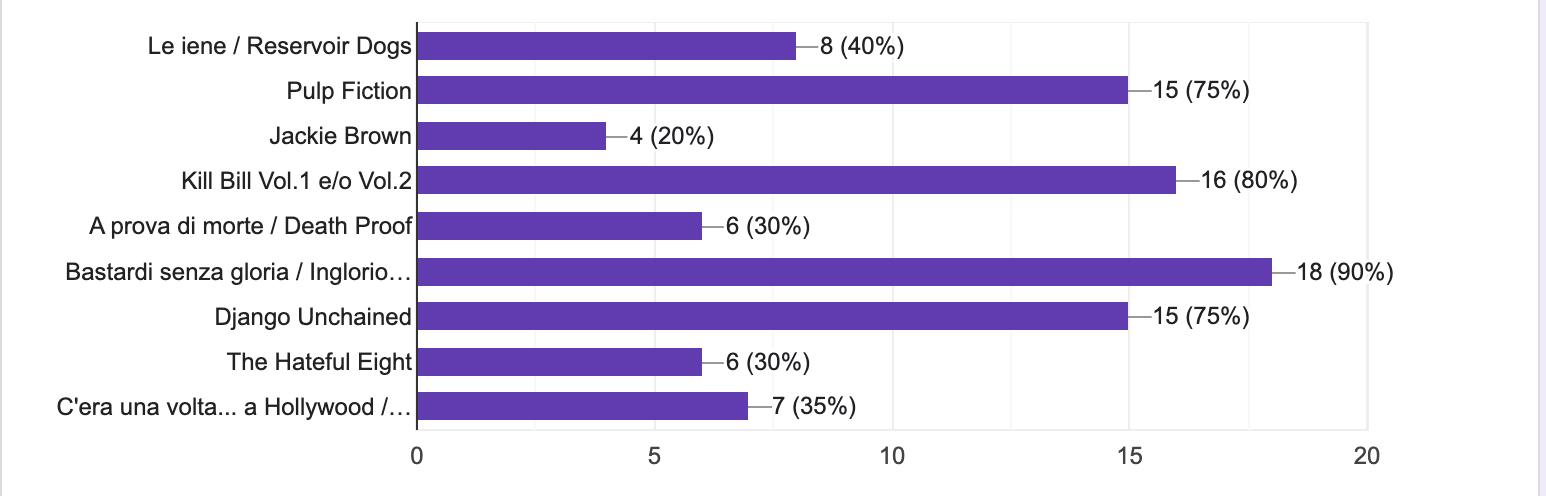
\includegraphics[width = 15cm, height = 5cm]{grafico1.png}
\end{figure}
Dall'indagine emerge che il film più visto in assoluto dai partecipanti è Inglorious Basterds, con una sorprendente percentuale del 90\%. 
Subito dopo si colloca la saga di Kill Bill, seguita a pari merito da Pulp Fiction e Django Unchained.  
I film meno visti, e apprezzati principalmente da appassionati, sono Jackie Brown (20\%), Death Proof (30\%) e The Hateful Eight (30\%). 
Anche il più recente Once Upon a Time in Hollywood registra un numero limitato di spettatori, raggiungendo solo il 35\%.  
La prevalenza di Kill Bill e Pulp Fiction tra le risposte può essere attribuita all’enorme impatto che questi film hanno avuto sulla cultura pop degli ultimi decenni, rendendoli iconici e facilmente riconoscibili. 
Al contrario, la popolarità di Inglorious Basterds e Django Unchained sembra legata al periodo in cui sono usciti, un’epoca in cui l’esperienza cinematografica era ancora molto diffusa, poiché le piattaforme di streaming non avevano ancora preso piede.  
Un ulteriore elemento da considerare è l’età dei partecipanti all’indagine, che si collocano prevalentemente nella fascia tra i 22 e i 30 anni. 
Questo dato contribuisce a spiegare l’interesse maggiore per i film di Tarantino più conosciuti e culturalmente rilevanti per questa generazione.
\end{flushleft}
\break

\subsubsection*{Quale tra questi è il tuo preferito?}
\begin{flushleft}
\begin{figure}[H]
    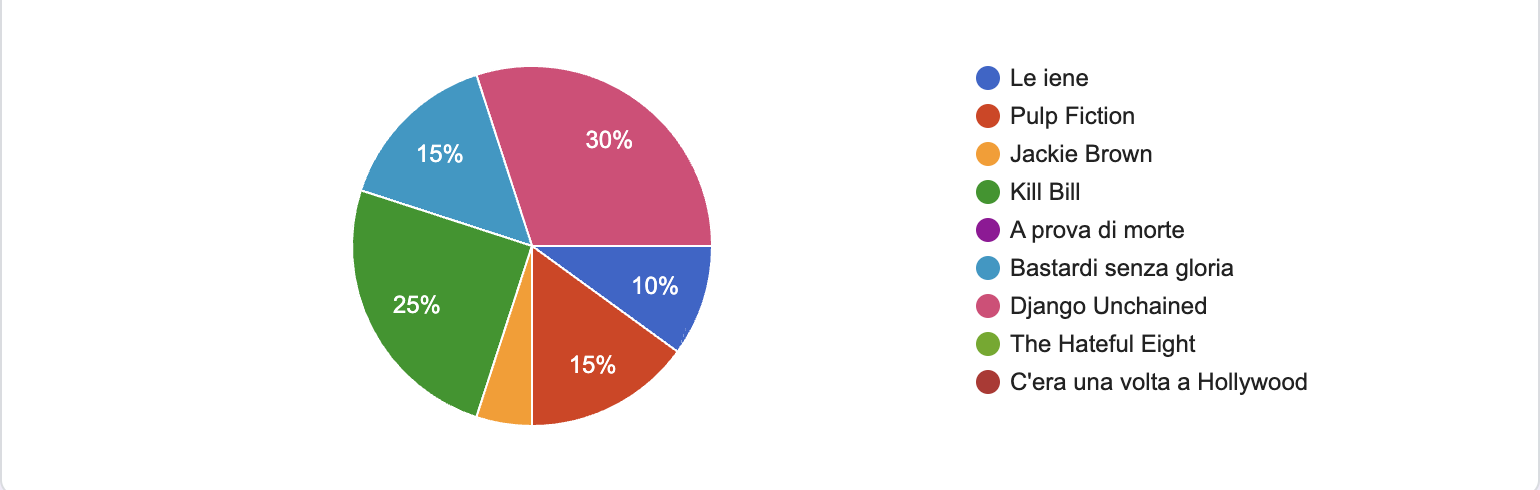
\includegraphics[width = 15cm, height = 5cm]{grafico2.png}
\end{figure}
Dal grafico si osserva che i quattro film più apprezzati sono quelli della saga di Kill Bill, insieme a Pulp Fiction, Inglorious Basterds e Django Unchained. 
Una piccola percentuale di partecipanti ha invece mostrato una preferenza per Reservoir Dogs e Jackie Brown.
Nessuno ha scelto Death Proof, The Hateful Eight o Once Upon a Time in Hollywood.  
Il vincitore assoluto in questa categoria è Django Unchained, scelto come film preferito dal 30\% dei partecipanti. Merita una menzione speciale anche Reservoir Dogs, il primo film diretto da Tarantino, che risulta il preferito per il 10\% degli intervistati.  
Questi risultati si allineano con i dati riportati nel paragrafo precedente, confermando le tendenze emerse riguardo alla popolarità dei film di Tarantino.
\end{flushleft}
\break

\subsubsection*{Scegli almeno una tra queste citazioni, altrimenti scrivine una te}
\begin{flushleft}
\begin{figure}[H]
    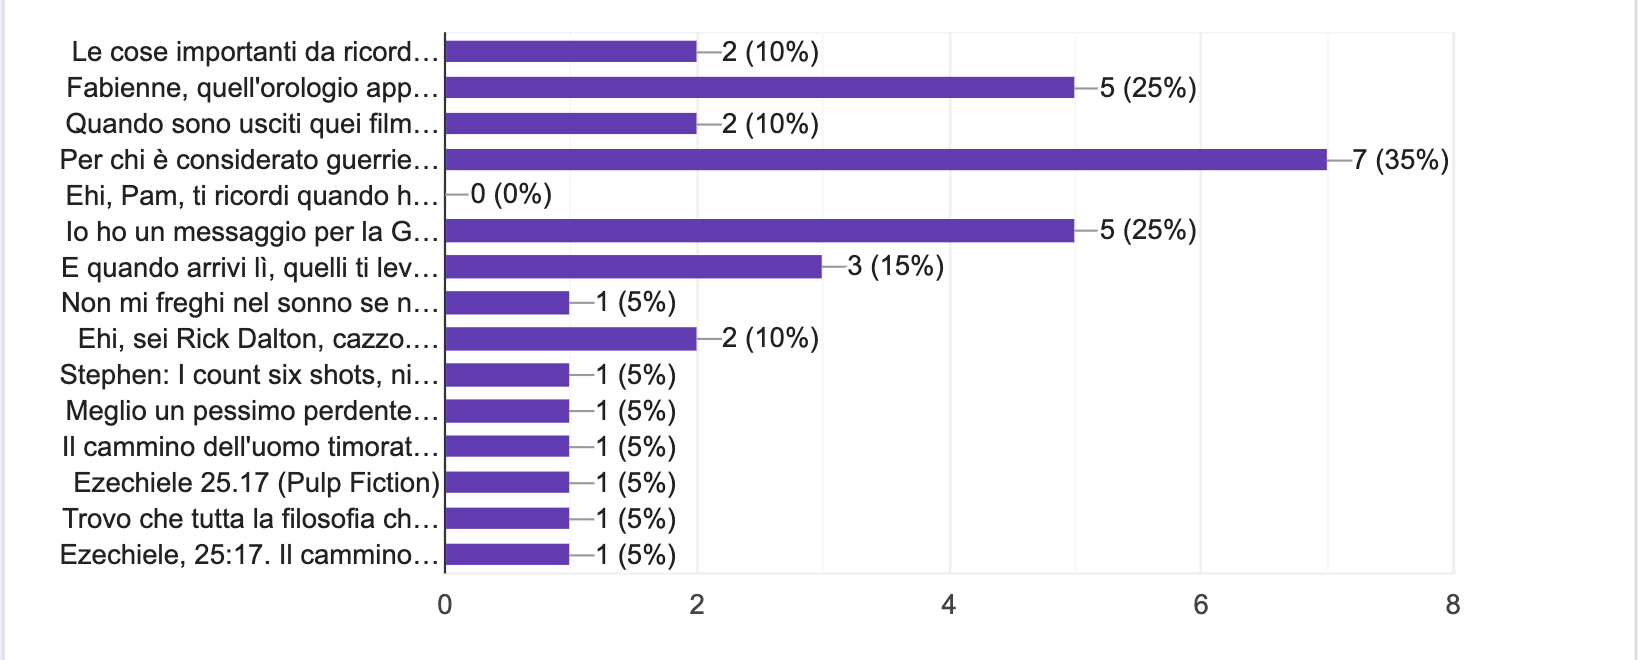
\includegraphics[width = 15cm, height = 6cm]{grafico3.png}
\end{figure}
Le citazioni scelte da me, una per film, erano le seguenti.
\begin{enumerate}
    \item Le cose importanti da ricordare sono i dettagli, i dettagli rendono la storia credibile. Questa particolare storia si svolge in un cesso pubblico, perciò devi conoscere tutto di quel cesso pubblico. Devi sapere se c'erano gli asciugamani di carta oppure il getto d'aria calda, devi sapere se i pisciatoi avevano le porte oppure no, devi sapere se c'era il sapone liquido o quella schifosissima polvere rosa che si usava al liceo, ricordi? Devi sapere se c'era o no l'acqua calda, se c'era puzza, se qualche pezzo di stronzo schifoso bastardo figlio di puttana aveva schizzato di diarrea una delle tazze. Devi sapere tutto quello che riguarda quel cesso, capito? (Reservoir Dogs)
    \item Fabienne, quell'orologio apparteneva a mio padre: hai idea di quante ne ha passate per farmi avere quell'orologio? Non ho tempo per i dettagli, ma ne ha passate un sacco. Ora, tutte queste stronzate le puoi anche bruciare, ma ti ho espressamente raccomandato di non dimenticarti di quel cazzo di orologio! (Pulp Fiction)
    \item Quando sono usciti quei film di Hong Kong non c'era fratello in giro che non volesse la .45; non gliene bastava una, ne volevano due per ripetere la scena dell'assassino. Ma in quei film del cazzo si guardano dal dirti che la .45 ha un piccolo difettuccio, e cioè che si inceppa. Io cerco di indirizzare il cliente verso la 9MM perché è maledettamente simile alla .45 ma pone molti meno problemi, però lo sai come sono fatti i negri: non riesci a farli ragionare, vogliono quella e basta. L'assassino aveva la .45? E quindi la vogliono anche loro. (Jackie Brown)
    \item Per chi è considerato guerriero, durante il combattimento l'annientamento del nemico deve essere l'unica preoccupazione. Reprimete qualsiasi emozione o compassione. Uccidete chiunque vi ostacoli, ancorché fosse Dio, o Buddha in persona. Questo è il cuore dell'arte del combattimento. (Kill Bill)
    \item Ehi, Pam, ti ricordi quando ho detto che quest'auto era a prova di morte? Non dicevo una bugia... quest'auto è al cento per cento a prova di morte. Ma per godere di questo vantaggio, tesoro, dovresti essere seduta esattamente dove sono io! (Death Proof)
    \item Io ho un messaggio per la Germania: voi state per morire tutti. E voglio che guardiate bene in faccia l'ebrea che vi ucciderà. (Inglorious Basterds)
    \item E quando arrivi lì, quelli ti levano il nome. Ti danno un numero e una mazza in mano, e dicono "Al lavoro!". Una parola insolente e ti tagliano la lingua, e lo sanno fare bene, non perdi sangue. Ohh, lo sanno fare benissimo. Ti fanno lavorare. Ogni giorno, per tutto il giorno, finché ti spacchi la schiena. Quel giorno ti danno un colpo di mazza e ti buttano nella fossa dei negri. E quella sarà la fine della tua storia, Django. (Django Unchained)
    \item Non mi freghi nel sonno se non chiudo mai gli occhi. (The Hateful Eight)
    \item Ehi, sei Rick Dalton, cazzo. Non scordartelo. (Once Upon a Time in Hollywood)
\end{enumerate}
Tra queste, la citazione preferita è stata sicuramente quella di Kill Bill (35\%). A parimerito, la citazione dell'orologio di Pulp Fiction e quella di Shosanna in Inglorious Basterds, apprezzate dal 25\% dei partecipanti.
Le restanti citazioni sono state scelte in modo misto, sottolineando il fatto che la narrazione e il dialogo di Tarantino riescono in qualche modo a fare breccia nelle persone.
Avevo inoltre dato la possibilità di scegliere una citazione a piacere.
Le citazioni emerse con questa modalità sono le seguenti.
\begin{enumerate}
    \item Stephen: \textit{Conto sei colpi, negro}.  Django: \textit{[Tira fuori una seconda revolver] Io conto due pistole, negro}. (Django Unchained)
    \item Meglio un pessimo perdente che un becero vincente. (Django Unchained)
    \item Ezechiele, 25:17. Il cammino dell'uomo timorato è minacciato da ogni parte dalle iniquità degli esseri egoisti e dalla tirannia degli uomini malvagi. Benedetto sia colui che nel nome della carità e della buona volontà, conduce i deboli attraverso la valle delle tenebre, perché egli è in verità il pastore di suo fratello e il ricercatore dei figli smarriti. E la mia giustizia calerà sopra di loro con grandissima vendetta e furiosissimo sdegno su coloro che si proveranno ad ammorbare, e infine a distruggere i miei fratelli. E tu saprai che il mio nome è quello del Signore, quando farò calare la mia vendetta sopra di te! (Pulp Fiction) 
    \item ...ma vorrei farti una domanda: quando avrai quel tuo posticino sull'isola di Nantucket... Immagino che vorrai toglierti la tua elegante uniforme da SS, è vero?  È quello che pensavo. Ecco, questo non lo sopporto! ...E tu Utivich? Tu lo sopporti? \textit{Nemmeno un po' signore}. Insomma, se facessimo a modo mio porteresti questa uniforme per il resto della tua vita da succhiacazzi, ma mi rendo conto che non è pratico e a un certo punto te la toglieresti: così ti darò una cosetta che non ti potrai togliere! (Inglorious Basterds)
    \item Trovo che tutta la filosofia che circonda i supereroi sia affascinante. Prendi il mio supereroe preferito: Superman. Non un grandissimo fumetto, la sua grafica è mediocre. Ma la filosofia, la filosofia non è soltanto eccelsa, è unica! Dunque, l'elemento fondamentale della filosofia dei supereroi è che abbiamo un supereroe e un suo alter-ego: Batman è di fatto Bruce Waine, l'Uomo Ragno è di fatto Peter Parker. Quando quel personaggio si sveglia al mattino è Peter Parker, deve mettersi un costume per diventare l'Uomo Ragno. Ed è questa caratteristica che fa di Superman l'unico nel suo genere: Superman non diventa Superman, lui è nato Superman, quando Superman si sveglia al mattino è Superman, il suo alter-ego è Clark Kent. Quella tuta con la grande ``S" rossa è la coperta che lo avvolgeva da bambino quando i Kent lo trovarono, sono quelli i suoi vestiti; quello che indossa come Kent, gli occhiali, l'abito da lavoro, quello è il suo costume, è il costume che Superman indossa per mimetizzarsi tra noi. Clark Kent è il modo in cui Superman ci vede; e quali sono le caratteristiche di Clark Kent?! È debole, non crede in sé stesso ed è un vigliacco. Clark Kent rappresenta la critica di Superman alla razza umana. (Kill Bill Vol.2)
\end{enumerate}
Di queste, il passaggio biblico di Pulp Fiction è stato citato spontaneamente da 3 partecipanti su 20.

\end{flushleft}
\break

\renewcommand{\refname}{}
\section {Sitografia}
\begin{flushleft}
    \small
    \begin{enumerate}
        \item \href{https://en.wikipedia.org/wiki/Quentin_Tarantino}{en.wikipedia.org/wiki/Quentin\_Tarantino}
        \item \href{https://https://www.biography.com/movies-tv/quentin-tarantino}{https://www.biography.com/movies-tv/quentin-tarantino}
        \item \href{https://en.wikipedia.org/wiki/Gunsmoke}{en.wikipedia.org/wiki/Gunsmoke}
        \item \href{https://it.wikipedia.org/wiki/Conoscenza_carnale}{it.wikipedia.org/wiki/Conoscenza\_carnale}
        \item \href{https://it.wikipedia.org/wiki/Deliverance}{it.wikipedia.org/wiki/Deliverance}
        \item \href{https://it.wikipedia.org/wiki/Sergio_Leone}{it.wikipedia.org/wiki/Sergio\_Leone}
        \item \href{https://it.wikipedia.org/wiki/Western_all%27italiana}{it.wikipedia.org/wiki/Western\_all\%27italiana}
        \item \href{https://en.wikipedia.org/wiki/Smokey_and_the_Bandit}{en.wikipedia.org/wiki/Smokey\_and\_the\_Bandit}
        \item \href{https://origintheatrical.com.au/work/11031}{origintheatrical.com.au/work/11031}
        \item \href{https://en.wikipedia.org/wiki/Roger_Avary}{en.wikipedia.org/wiki/Roger\_Avary}
        \item \href{https://en.wikipedia.org/wiki/Danny_Strong}{en.wikipedia.org/wiki/Danny\_Strong}
        \item \href{https://en.wikipedia.org/wiki/Allen_Garfield}{en.wikipedia.org/wiki/Allen\_Garfield}
        \item \href{https://www.corriere.it/spettacoli/cinema-serie-tv/cards/quentin-tarantino-compie-60-anni-origini-italiane-rapporto-uma-thurman-altri-segreti-di-lui/lavoro-videonoleggio.shtml}{Il lavoro al videonoleggio, Arianna Ascione, Corriere della Sera, 27 marzo 2023}
        \item \href{https://en.wikipedia.org/wiki/My_Best_Friend%27s_Birthday}{https://en.wikipedia.org/wiki/My\_Best\_Friend\%27s\_Birthday}
        \item \href{https://en.wikipedia.org/wiki/True_Romance}{https://en.wikipedia.org/wiki/True\_Romance}
        \item \href{https://en.wikipedia.org/wiki/Natural_Born_Killers}{https://en.wikipedia.org/wiki/Natural\_Born\_Killers}
        \item \href{https://it.wikipedia.org/wiki/Avantpop_(movimento_artistico)}{https://it.wikipedia.org/wiki/Avantpop\_\(movimento_artistico\)}
        \item \href{https://it.wikipedia.org/wiki/Dal_tramonto_all%27alba}{https://it.wikipedia.org/wiki/Dal\_tramonto\_all\%27alba}
        \item \href{https://it.wikipedia.org/wiki/Getaway!}{https://it.wikipedia.org/wiki/Getaway!}
        \item \href{https://en.wikipedia.org/wiki/Night_of_the_Living_Dead}{https://en.wikipedia.org/wiki/Night\_of\_the\_Living\_Dead}
        \item \href{https://ilregnodeglianni80.forumfree.it/?t=62030520}{https://ilregnodeglianni80.forumfree.it/?t=62030520}
        \item \href{https://it.wikipedia.org/wiki/Script_doctor}{https://it.wikipedia.org/wiki/Script\_doctor}
        \item \href{https://en.wikipedia.org/wiki/Past_Midnight}{https://en.wikipedia.org/wiki/Past\_Midnight}
        \item \href{https://en.wikipedia.org/wiki/Heist_film}{https://en.wikipedia.org/wiki/Heist\_film}
        \item \href{https://it.wikipedia.org/wiki/Monte_Hellman}{https://it.wikipedia.org/wiki/Monte\_Hellman}
        \item \href{https://it.wikipedia.org/wiki/Lions_Gate_Entertainment}{https://it.wikipedia.org/wiki/Lions\_Gate\_Entertainment}
        \item \href{https://en.wikipedia.org/wiki/Harvey_Keitel}{https://en.wikipedia.org/wiki/Harvey\_Keitel}
        \item \href{https://www.sundance.org/}{https://www.sundance.org/}
        \item \href{https://en.wikipedia.org/wiki/Alfred_Hitchcock_Presents}{https://en.wikipedia.org/wiki/Alfred\_Hitchcock\_Presents}
        \item \href{https://en.wikipedia.org/wiki/Desperado_(film)}{https://en.wikipedia.org/wiki/Desperado\_\(film\)}
        \item \href{https://www.odgmagazine.com/il-mito-della-blaxploitation/}{Il mito della Blaxploitation, ODG, Andrea Tiradritti, 19 marzo 2021}
        \item \href{https://en.wikipedia.org/wiki/Steven_Spielberg%27s_Director%27s_Chair}{https://en.wikipedia.org/wiki/Steven\_Spielberg's\_Director's\_Chair}
        \item \href{https://en.wikipedia.org/wiki/Wait_Until_Dark}{https://en.wikipedia.org/wiki/Wait\_Until\_Dark}
        \item \href{https://www.imdb.com/name/nm0000235/bio/}{https://www.imdb.com/name/nm0000235/bio/}
        \item \href{https://www.miramax.com/}{https://www.miramax.com/}
        \item \href{https://en.wikipedia.org/wiki/CSI:_Crime_Scene_Investigation}{https://en.wikipedia.org/wiki/CSI:\_Crime\_Scene\_Investigation}
        \item \href{http://www.cineforumimperia.it/file/cine_RUBRICHE/rub_approfondimenti/uno_sguardo/sg_exploitation.html}{http://www.cineforumimperia.it/file/exploitation.html}
        \item \href{https://www.studiobinder.com/blog/what-is-a-grindhouse-movie-definition/}{https://www.studiobinder.com/blog/what-is-a-grindhouse-movie-definition/}
        \item \href{https://en.wikipedia.org/wiki/The_Inglorious_Bastards}{https://en.wikipedia.org/wiki/The\_Inglorious\_Bastards}
        \item \href{https://en.wikipedia.org/wiki/Extra_(American_TV_program)}{https://en.wikipedia.org/wiki/Extra}
        \item \href{https://www.comic-con.org/}{https://www.comic-con.org/}
        \item \href{https://en.wikipedia.org/wiki/The_Weinstein_Company}{https://en.wikipedia.org/wiki/The\_Weinstein\_Company}
        \item \href{https://www.rainews.it/photogallery/2023/03/il-cinema--rock-and-roll-i-60-anni-di-quentin-tarantino-35b729db-7cc9-4b1b-a3cf-235bc05a55e6.html}{Il cinema è rock and roll: i 60 anni di Quentin Tarantino, RaiNews, 27 marzo 2023}
        \item \href{https://www.radiocinema.it/news/quentin-tarantino-altri-tre-film-lascio-il-cinema}{Quentin Tarantino: altri tre film e lascio il cinema, Radio Cinema, 11 novembre 2014}
        \item \href{https://en.wikipedia.org/wiki/My_Best_Friend%27s_Birthday}{https://en.wikipedia.org/wiki/My\_Best\_Friends\_Birthday}
        \item \href{https://wiki.tarantino.info/index.php/My_Best_Friend%27s_Birthday}{https://wiki.tarantino.info/index.php/My\_Best\_Friends\_Birthday}
        \item \href{https://indiefilmhustle.com/quentin-tarantino-best-friends-birthday/}{https://indiefilmhustle.com/quentin-tarantino-best-friends-birthday/}
        \item \href{https://it.wikipedia.org/wiki/Rockabilly}{https://it.wikipedia.org/wiki/Rockabilly}
        \item \href{https://it.wikipedia.org/wiki/Surf_music}{https://it.wikipedia.org/wiki/Surf\_music}
        \item \href{https://en.wikipedia.org/wiki/Reservoir_Dogs}{https://en.wikipedia.org/wiki/Reservoir\_Dogs}
        \item \href{https://www.rottentomatoes.com/m/reservoir_dogs}{https://www.rottentomatoes.com/m/reservoir\_dogs}
        \item \href{https://www.rogerebert.com/reviews/reservoir-dogs-1992}{https://www.rogerebert.com/reviews/reservoir-dogs-1992}
        \item \href{https://www.newyorker.com/culture/cultural-comment/the-glorious-bullshit-of-reservoir-dogs-twenty-five-years-later}{The Glorious Bullshit of Reservoir Dogs Twenty Five Years Later, Tom Shone, Newyorker, 8 ottobre 2017}
        \item \href{https://wiki.tarantino.info/index.php/Reservoir_Dogs_movie_references_guide}{https://wiki.tarantino.info/index.php/ReservoirDogs\_references}
        \item \href{https://it.wikipedia.org/wiki/City_on_Fire_(film_1987)}{https://it.wikipedia.org/wiki/City\_on\_Fire}
        \item \href{https://www.treccani.it/enciclopedia/triello_(altro)/}{https://www.treccani.it/enciclopedia/triello/}
        \item \href{https://www.progettohmr.it/Retrologico/026-citazione-picasso/}{https://www.progettohmr.it/Retrologico/026-citazione-picasso/}
        \item \href{https://it.wikipedia.org/wiki/L%27arrivo_di_un_treno_alla_stazione_di_La_Ciotat}{https://it.wikipedia.org/wiki/arrivodiun\_treno\_La\_Ciotat}
        \item \href{https://sitgesfilmfestival.com/en}{https://sitgesfilmfestival.com/en}
        \item \href{https://it.wikipedia.org/wiki/Pulp_Fiction}{https://it.wikipedia.org/wiki/Pulp\_Fiction}
        \item \href{https://wiki.tarantino.info/index.php/Pulp_Fiction_Movie_References_Guide}{https://wiki.tarantino.info/index.php/Pulp\_Fiction\_References}
        \item \href{https://ahdictionary.com/word/search.html?q=pulp}{https://ahdictionary.com/word/search.html?q=pulp}
        \item \href{https://sony.fandom.com/wiki/TriStar_Pictures}{https://sony.fandom.com/wiki/TriStar\_Pictures}
        \item \href{https://movieplayer.it/articoli/roger-avary-pulp-fiction-intervista_22689/}{Roger Avary e Pulp Fiction: “Quando vinsi l’Oscar mi scappava la pipì”, Max Borg, Movie Player, 27 marzo 2020}
        \item \href{https://www.loc.gov/programs/national-film-preservation-board/film-registry/complete-national-film-registry-listing/}{https://www.loc.gov/programs/complete-national-film-registry-listing/}
        \item \href{https://it.wikipedia.org/wiki/Jackie_Brown}{https://it.wikipedia.org/wiki/Jackie\_Brown}
        \item \href{https://wiki.tarantino.info/index.php/Jackie_Brown_movie_and_TV_references_guide}{https://wiki.tarantino.info/index.php/Jackie\_Brown\_References}
        \item \href{https://it.wikipedia.org/wiki/Punch_al_rum}{https://it.wikipedia.org/wiki/Punch\_al\_rum}
        \item \href{https://it.wikipedia.org/wiki/Elmore_Leonard}{https://it.wikipedia.org/wiki/Elmore\_Leonard}
        \item \href{https://it.wikipedia.org/wiki/Out_of_Sight_(film)}{https://it.wikipedia.org/wiki/OutOfSight}
        \item \href{https://it.wikipedia.org/wiki/Kill_Bill:_Volume_1}{https://it.wikipedia.org/wiki/Kill\_Bill:\_Volume\_1}
        \item \href{https://en.wikipedia.org/wiki/Kill_Bill:_Volume_2}{https://en.wikipedia.org/wiki/Kill\_Bill:\_Volume\_2}
        \item \href{https://wiki.tarantino.info/index.php/Kill_Bill_References_Guide}{https://wiki.tarantino.info/index.php/Kill\_Bill\_References\_Guide}
        \item \href{https://en.wikipedia.org/wiki/Samurai_cinema}{https://en.wikipedia.org/wiki/Samurai\_cinema}
        \item \href{https://it.wikipedia.org/wiki/Chang_Cheh}{https://it.wikipedia.org/wiki/Chang\_Cheh}
        \item \href{https://it.wikipedia.org/wiki/Super_8_millimetri}{https://it.wikipedia.org/wiki/Super\_8\_millimetri}
        \item \href{https://it.wikipedia.org/wiki/Grindhouse}{https://it.wikipedia.org/wiki/Grindhouse}
        \item \href{https://en.wikipedia.org/wiki/Planet_Terror}{https://en.wikipedia.org/wiki/Planet\_Terror}
        \item \href{https://en.wikipedia.org/wiki/Death_Proof}{https://en.wikipedia.org/wiki/Death\_Proof}
        \item \href{https://wiki.tarantino.info/index.php/Grindhouse_movie_references_guide}{https://wiki.tarantino.info/index.php/Grindhouse}
        \item \href{https://it.wikipedia.org/wiki/Bastardi_senza_gloria}{https://it.wikipedia.org/wiki/Bastardi\_senza\_gloria}
        \item \href{https://wiki.tarantino.info/index.php/Inglourious_Basterds_movie_references_guide}{https://wiki.tarantino.info/index.php/Inglourious\_Basterds}
        \item \href{https://it.wikipedia.org/wiki/Django_Unchained}{https://it.wikipedia.org/wiki/Django\_Unchained}
        \item \href{https://wiki.tarantino.info/index.php/Django_Unchained_Movie_References_guide}{https://wiki.tarantino.info/index.php/Django\_Unchained}
        \item \href{https://it.wikipedia.org/wiki/Django_(film_1966)}{https://it.wikipedia.org/wiki/Django}
        \item \href{https://it.wikipedia.org/wiki/Trilogia_del_tempo}{https://it.wikipedia.org/wiki/Trilogia\_del\_tempo}
        \item \href{https://it.wikipedia.org/wiki/L%27anello_del_Nibelungo}{https://it.wikipedia.org/wiki/anello\_del\_Nibelungo}
        \item \href{https://www.cinefacts.it/cinefacts-articolo-1597/django-unchained-la-fiaba-grottesca-e-rovesciata-di-un-sigfrido-del-west.html}{Django Unchained - La fiaba grottesca e rovesciata di un Sigfrido del West, Silvia Argento, Cinefacts, 17 gennaio 2024}
        \item \href{https://it.wikipedia.org/wiki/The_Hateful_Eight}{https://it.wikipedia.org/wiki/The\_Hateful\_Eight}
        \item \href{https://wiki.tarantino.info/index.php/The_Hateful_Eight_Movie_References_guide}{https://wiki.tarantino.info/index.php/The\_Hateful\_Eight}
        \item \href{https://it.wikipedia.org/wiki/Bonanza}{https://it.wikipedia.org/wiki/Bonanza}
        \item \href{https://it.wikipedia.org/wiki/Il_virginiano}{https://it.wikipedia.org/wiki/Il\_virginiano}
        \item \href{https://en.wikipedia.org/wiki/The_High_Chaparral}{https://en.wikipedia.org/wiki/The\_High\_Chaparral}
        \item \href{https://en.wikipedia.org/wiki/American_International_Pictures}{https://en.wikipedia.org/wiki/American\_International\_Pictures}
        \item \href{https://it.wikipedia.org/wiki/Pam_Grier}{https://it.wikipedia.org/wiki/Pam\_Grier}
        \item \href{https://it.wikipedia.org/wiki/Foxy_Brown_(film)}{https://it.wikipedia.org/wiki/Foxy\_Brown}
        \item \href{https://it.wikipedia.org/wiki/Sesso_in_gabbia}{https://it.wikipedia.org/wiki/Sesso\_in\_gabbia}
        \item \href{https://en.wikipedia.org/wiki/TNT_Jackson}{https://en.wikipedia.org/wiki/TNT\_Jackson}
        \item \href{https://it.wikipedia.org/wiki/Rolling_Thunder_(film_1977)}{https://it.wikipedia.org/wiki/Rolling\_Thunder}
        \item \href{https://it.wikipedia.org/wiki/Buio_oltre_il_sole}{https://it.wikipedia.org/wiki/Buio\_oltre\_il\_sole}
        \item \href{https://en.wikipedia.org/wiki/The_Legend_of_Nigger_Charley}{https://en.wikipedia.org/wiki/The\_Legend\_of\_Nigger\_Charley}
        \item \href{https://it.wikipedia.org/wiki/Batman_(film_1966)}{https://it.wikipedia.org/wiki/Batman}
        \item \href{https://it.wikipedia.org/wiki/Ghost_in_the_Shell_(film_1995)}{https://it.wikipedia.org/wiki/Ghost\_in\_the\_Shell}
        \item \href{https://simpsons.fandom.com/wiki/Reservoir_Cats}{https://simpsons.fandom.com/wiki/Reservoir\_Cats}
        \item \href{https://it.wikipedia.org/wiki/Il_colpo_della_metropolitana_(Un_ostaggio_al_minuto)}{https://it.wikipedia.org/wiki/Il\_colpo\_della\_metropolitana}
        \item \href{https://www.torinofilmfest.org/it/11-festival-internazionale-cinema-giovani/film/the-lodger-/-a-story-of-the-london-fog/2473/}{https://www.torinofilmfest.org/thelodger}
        \item \href{https://www.moma.org/collection/works/304708}{https://www.moma.org/collection/works/304708}
        \item \href{https://it.wikipedia.org/wiki/Via_col_vento}{https://it.wikipedia.org/wiki/Via\_col\_vento}
        \item \href{https://www.esquire.com/entertainment/movies/news/a41379/quentin-tarantino-movies-connected/}{All Quentin Tarantino Movies Are Connected, Matt Miller, Esquire, 26 luglio 2019}
        \item \href{https://www.cbr.com/quentin-tarantino-movie-connections-explained/}{The Connections Between Quentin Tarantino's Movies, Sean Alexander \& Arthur Goyaz, CBR, 2 dicembre 2024}
        \item \href{https://it.wikipedia.org/wiki/Neoliberismo}{https://it.wikipedia.org/wiki/Neoliberismo}
        \item \href{https://it.wikipedia.org/wiki/Ronald_Reagan}{https://it.wikipedia.org/wiki/Ronald\_Reagan}
        \item \href{https://it.wikipedia.org/wiki/Storia_degli_Stati_Uniti_d%27America_(1988-presente)}{https://it.wikipedia.org/wiki/Stati\_Uniti\_dAmerica\_1988-presente}
        \item \href{https://it.wikipedia.org/wiki/Seconda_guerra_mondiale}{https://it.wikipedia.org/wiki/Seconda\_guerra\_mondiale}
        \item \href{https://it.wikipedia.org/wiki/Guerra_civile_americana}{https://it.wikipedia.org/wiki/Guerra\_civile\_americana}
        \item \href{https://it.wikipedia.org/wiki/Era_della_ricostruzione}{https://it.wikipedia.org/wiki/Era\_della\_ricostruzione}
        \item \href{https://en.wikipedia.org/wiki/Reservoir_Dogs_(soundtrack)}{https://en.wikipedia.org/wiki/Reservoir\_Dogs\_Soundtrack}
        \item \href{https://en.wikipedia.org/wiki/Pulp_Fiction_(soundtrack)}{https://en.wikipedia.org/wiki/Pulp\_Fiction\_Soundtrack}
        \item \href{https://en.wikipedia.org/wiki/Jackie_Brown:_Music_from_the_Miramax_Motion_Picture}{https://en.wikipedia.org/wiki/Jackie\_Brown\_Soundtrack}
        \item \href{https://en.wikipedia.org/wiki/Kill_Bill_Vol._1_Original_Soundtrack}{https://en.wikipedia.org/wiki/Kill\_Bill\_Vol1\_Original\_Soundtrack}
        \item \href{https://it.wikipedia.org/wiki/Wu-Tang_Clan}{https://it.wikipedia.org/wiki/WuTang\_Clan}
        \item \href{https://en.wikipedia.org/wiki/Inglourious_Basterds_(soundtrack)}{https://en.wikipedia.org/wiki/Inglourious\_Basterds\_soundtrack}
        \item \href{https://en.wikipedia.org/wiki/Django_Unchained_(soundtrack)}{https://en.wikipedia.org/wiki/Django\_Unchained\_soundtrack}
        \item \href{https://en.wikipedia.org/wiki/Hi_Diddle_Diddle}{https://en.wikipedia.org/wiki/Hi\_Diddle\_Diddle}
        \item \href{https://en.wikipedia.org/wiki/Cat_People_(1942_film)}{https://en.wikipedia.org/wiki/Cat\_People}
        \item \href{https://it.wikipedia.org/wiki/The_Millionaire_(film_2008)}{https://it.wikipedia.org/wiki/The\_Millionaire}
        \item \href{https://en.wikipedia.org/wiki/The_Hateful_Eight_(soundtrack)}{https://en.wikipedia.org/wiki/The\_Hateful\_Eight\_soundtrack}
        \item \href{https://en.wikipedia.org/wiki/Buddy_Goes_West}{https://en.wikipedia.org/wiki/Buddy\_Goes\_West}
        \item \href{https://it.wikipedia.org/wiki/Il_gioco_di_Ripley}{https://it.wikipedia.org/wiki/Il\_gioco\_di\_Ripley}
        \item \href{https://it.wikipedia.org/wiki/La_cosa_(film_1982)}{https://it.wikipedia.org/wiki/La\_cosa}
        \item \href{https://en.wikipedia.org/wiki/Exorcist_II:_The_Heretic}{https://en.wikipedia.org/wiki/ExorcistII}
        \item \href{https://en.wikipedia.org/wiki/Once_Upon_a_Time_in_Hollywood_(soundtrack)}{https://en.wikipedia.org/wiki/Once\_Upon\_a\_Time\_Soundtrack}
        \item \href{https://variety.com/lists/best-quentin-tarantino-characters/}{The Best Quentin Tarantino Characters, From ‘Pulp Fiction’ to ‘Kill Bill’, Variety, 27 marzo 2023}
        \end{enumerate}
\end{flushleft}
\break

\end{document}
